% Options for packages loaded elsewhere
\PassOptionsToPackage{unicode}{hyperref}
\PassOptionsToPackage{hyphens}{url}
\documentclass[
]{article}
\usepackage{xcolor}
\usepackage{amsmath,amssymb}
\setcounter{secnumdepth}{-\maxdimen} % remove section numbering
\usepackage{iftex}
\ifPDFTeX
  \usepackage[T1]{fontenc}
  \usepackage[utf8]{inputenc}
  \usepackage{textcomp} % provide euro and other symbols
\else % if luatex or xetex
  \usepackage{unicode-math} % this also loads fontspec
  \defaultfontfeatures{Scale=MatchLowercase}
  \defaultfontfeatures[\rmfamily]{Ligatures=TeX,Scale=1}
\fi
\usepackage{lmodern}
\ifPDFTeX\else
  % xetex/luatex font selection
\fi
% Use upquote if available, for straight quotes in verbatim environments
\IfFileExists{upquote.sty}{\usepackage{upquote}}{}
\IfFileExists{microtype.sty}{% use microtype if available
  \usepackage[]{microtype}
  \UseMicrotypeSet[protrusion]{basicmath} % disable protrusion for tt fonts
}{}
\makeatletter
\@ifundefined{KOMAClassName}{% if non-KOMA class
  \IfFileExists{parskip.sty}{%
    \usepackage{parskip}
  }{% else
    \setlength{\parindent}{0pt}
    \setlength{\parskip}{6pt plus 2pt minus 1pt}}
}{% if KOMA class
  \KOMAoptions{parskip=half}}
\makeatother
\usepackage{longtable,booktabs,array}
\usepackage{tabularx}
\usepackage{enumitem}
\usepackage{lscape} % plain lscape (not pdflscape): keeps the page number
                     % upright and normally positioned on landscape pages
                     % instead of rotating it sideways with the content
\usepackage{float} % needed for [H] float placement (angle2_cohort.tex cohort table)
\usepackage{needspace} % keep the four-step sentence with its figure
\newcounter{none} % for unnumbered tables
\usepackage{calc} % for calculating minipage widths
% Correct order of tables after \paragraph or \subparagraph
\usepackage{etoolbox}
\makeatletter
\patchcmd\longtable{\par}{\if@noskipsec\mbox{}\fi\par}{}{}
\makeatother
% Allow footnotes in longtable head/foot
\IfFileExists{footnotehyper.sty}{\usepackage{footnotehyper}}{\usepackage{footnote}}
\makesavenoteenv{longtable}
\ifLuaTeX
  \usepackage{luacolor}
  \usepackage[soul]{lua-ul}
\else
  \usepackage{soul}
\fi
\setlength{\emergencystretch}{3em} % prevent overfull lines
\providecommand{\tightlist}{%
  \setlength{\itemsep}{0pt}\setlength{\parskip}{0pt}}
\usepackage{bookmark}
\IfFileExists{xurl.sty}{\usepackage{xurl}}{}
\IfFileExists{xltabular.sty}{\usepackage{xltabular}}{} % add URL line breaks if available
\urlstyle{same}
\hypersetup{
  hidelinks,
  pdfcreator={LaTeX via pandoc}}

\usepackage{tikz}
\usetikzlibrary{positioning,arrows.meta,shapes.geometric}
\usepackage{placeins} % \FloatBarrier: stop figures drifting past chapter
                       % boundaries (added after figures were found floating
                       % all the way past the bibliography into the appendix)
\newcommand{\fb}{\discretionary{}{}{}} % invisible break point for long
                       % underscore-joined filenames in narrow table columns

\author{}
\date{}

\begin{document}
\setlength{\LTleft}{\fill}\setlength{\LTright}{\fill} % center every
                       % longtable on the page (default is flush-left,
                       % which left tables sitting off-centre with a big
                       % gap on the right - notably in the appendices).
                       % Placed after \begin{document} so longtable's own
                       % initialisation doesn't clobber it.

\begin{titlepage}
  \centering
  \vspace*{4cm}

  {\LARGE\textbf{Build Once, Answer Many}\par}
  \vspace{1cm}
  {\large\emph{Where disclosure demand converges for European seafood-processing SMEs}\par}
  \vspace{0.5cm}
  {\large\emph{A diagnostic framework to transform compliance obligations into strategic advantage}\par}
  \vspace{2cm}
  {\large\textbf{Master's Thesis}\par}
  \vspace{1.5cm}
  {\large Linne Verhoeven\par}
  \vspace{0.8cm}
  {\large Supervised by Professor Jean-Philippe Bonardi\par}
  \vspace{0.4cm}
  {\large In collaboration with Seafood Europe\par}
  \vspace{1.2cm}
  {\large August 2026\par}
\end{titlepage}

\thispagestyle{empty}
\vspace*{2cm}
\begin{center}
{\Large\textbf{Acknowledgements}}
\end{center}
\vspace{1cm}
\noindent
I would like to thank my supervisor, Professor Jean-Philippe Bonardi, for his
guidance throughout this thesis.

I am grateful to the sustainability leads at Thai Union, Bolton Group, Nomad
Foods, Profand, A.~Espersen and Mowi, who gave their time to this research and
to whom the cohort coding underlying Chapter~5 has been submitted for review,
and to the industry contacts at Seafood Europe who discussed the instrument
landscape in Chapter~4 with me. I owe a particular debt to Antonio \'Alvarez, Director of Sustainability at
Profand, whose detailed review of Chapter~5 identified the indexing effect now
documented in Section~5.3. Any remaining errors are my own.

\clearpage

\begin{abstract}
\noindent
European SMEs face a fragmented wall of sustainability-disclosure demands.
Regulators, retail customers, certifiers, investors and NGOs each request
seemingly different information through different channels, and for a firm
with limited resources the rational response is reactive: answer the loudest
demand, defer the rest, and build nothing that would serve more than the
request in front of it. Yet beneath these superficially different requests
lies a far smaller set of recurring \emph{themes} and the \emph{datapoints}
that produce them. This thesis argues that a resource-constrained firm which
identifies the few themes on which demand converges - and learns to
generate their underlying datapoints once - can satisfy most of what it is
asked from a single effort, shifting from reactive compliance to proactive
strategy.


Taking European seafood processing as a case, the thesis demonstrates this in
four steps. Step~1 maps the sector's disclosure \emph{ecosystem}: 49 catalogued
regulatory, customer, investor and industry instruments, of which 30 place a
scorable demand on the firm. Step~2 establishes what mature firms actually
report, using six large processors from among the sector's most advanced reporters. Even
the deepest covers only 60 of 70 relevant ESRS disclosure requirements, and all
six converge on a 13-requirement core regardless of how differently they source
their fish.

Step~3 crosses the two, and is where the central finding appears. Scoring every
topic against every instrument yields 1{,}023 combinations, of which just 18 per cent
carry any demand at all. That sparse demand is heavily concentrated: a small set
of topics already answers most of what the ecosystem asks. What presents itself
as dozens of separate requests is, underneath, a handful of shared ones.

Step~4 turns this into a diagnostic. Topics are staged by how strongly and how
widely they are demanded, producing a four-topic core every seafood processor
should build first - energy, greenhouse-gas emissions, biodiversity and
supply-chain traceability - extending to nine topics for a mixed-sourcing firm,
eight for aquaculture and five for wild-capture. For the modelled firm, those
build-first topics answer a demand raised by 26 of the 30 frameworks scored in
the sector's landscape, from one dataset. The findings give seafood SMEs a sequenced
prioritisation framework and provide empirical input to the EU
sustainability-simplification debate.
\end{abstract}

\tableofcontents
\clearpage
\listoffigures
\listoftables
\clearpage

\section*{List of Abbreviations}
\addcontentsline{toc}{section}{List of Abbreviations}
\begin{description}[leftmargin=2.6cm,style=nextline]
\setlength{\itemsep}{2pt}
\item[ASC] Aquaculture Stewardship Council
\item[BAP] Best Aquaculture Practices
\item[CDP] Carbon Disclosure Project
\item[CSDDD] Corporate Sustainability Due Diligence Directive
\item[CSR] Corporate Social Responsibility
\item[CSRD] Corporate Sustainability Reporting Directive
\item[DR] Disclosure Requirement (ESRS)
\item[EC] European Commission
\item[EFRAG] European Financial Reporting Advisory Group
\item[ESG] Environmental, Social and Governance
\item[ESRS] European Sustainability Reporting Standards
\item[EU] European Union
\item[EUDR] EU Deforestation Regulation
\item[EU Taxonomy] EU classification system for environmentally sustainable
economic activities (Regulation (EU) 2020/852)
\item[EPR] Extended Producer Responsibility
\item[F-gas] Fluorinated Greenhouse Gas (EU F-gas Regulation)
\item[GDST] Global Dialogue on Seafood Traceability
\item[GHG] Greenhouse Gas
\item[GLOBALG.A.P.] Global Good Agricultural Practice
\item[GRI] Global Reporting Initiative
\item[GSSI] Global Sustainable Seafood Initiative
\item[IFRS S1/S2] IFRS Sustainability Disclosure Standards 1 and 2 (ISSB)
\item[ISSB] International Sustainability Standards Board
\item[ISO] International Organization for Standardization
\item[ISSF] International Seafood Sustainability Foundation
\item[IUU] Illegal, Unreported and Unregulated (fishing)
\item[MSC] Marine Stewardship Council
\item[NGO] Non-Governmental Organisation
\item[OSH] Occupational Safety and Health
\item[PPWR] Packaging and Packaging Waste Regulation
\item[RSPO] Roundtable on Sustainable Palm Oil
\item[SASB] Sustainability Accounting Standards Board
\item[SBTi] Science Based Targets initiative
\item[SFDR] Sustainable Finance Disclosure Regulation
\item[SME] Small and Medium-sized Enterprise
\item[SMETA] Sedex Members Ethical Trade Audit
\item[STECF] Scientific, Technical and Economic Committee for Fisheries
\item[TNFD] Taskforce on Nature-related Financial Disclosures
\item[UN] United Nations
\item[VSME] Voluntary Sustainability Reporting Standard for SMEs
\end{description}
\clearpage


% ===== Introduction. Sources still to add to references.tex / Zotero: =====
% - Afolabi, H., Ram, R. & Rimmel, G. (2022). Harmonization of Sustainability Reporting
%   Regulation: Analysis of a Contested Arena. Sustainability 14(9), 5517. doi:10.3390/su14095517
% - EFRAG (2021). ESRS / double materiality.        - EFRAG (2024). VSME standard.
% - European Commission (2025). VSME recommendation.
% - European Commission (2026). Revised ESRS + value-chain cap (Omnibus). finance.ec.europa.eu
% RESOLVED: The European House - Ambrosetti / TEHA Group (2026) STAGE Index citation
%   (main.tex ~line 260) -- verified real via web search + the link Ruben supplied:
%   https://www.ambrosetti.eu/en/news/sustainable-transition-non-negotiable-priorities-for-the-future-of-businesses/
%   2026 Strategic Report "Non-negotiable priorities for businesses and the future of
%   the sustainable transition" (TEHA Group / The European House-Ambrosetti, with Erion),
%   presented at the Erion Forum, Rome, 17 June 2026. The STAGE Index (Sustainable
%   Transition Alignment between Government & Enterprises) registers ~51% convergence
%   in 2026. In-text now names the index explicitly instead of "one practitioner index".
% RESOLVED: STECF (2025) 3,245-enterprise / two-thirds-micro / large-firm figures --
%   verified via web search against STECF 25-15 "Economic report on the fish processing
%   industry": 3,245 main-activity enterprises in 2023, ~67% microfirms (<10 employees),
%   large enterprises (250+) are ~2% of firms (~65, thesis says 66 -- a one-firm rounding
%   difference from the 2%-of-3,245 back-calculation; worth a 5-minute check against the
%   report's own table if you want the exact reported count rather than the recomputed one).
% RESOLVED: the "alphabet soup / harmonisation" cite at main.tex:414 now points to
%   Afolabi, Ram & Rimmel (2022), whose title is literally about this contested
%   harmonisation arena -- a tighter match than Adams & Abhayawansa. Verified real
%   via search: Sustainability 14(9), 5517, doi:10.3390/su14095517.
% RESOLVED: the "buyers drop suppliers over ESG data" line in 1.3 now cites
%   Tanase (2025), Veridion -- a real, dated industry source confirming ESG
%   screening/scoring gates suppliers out at exactly the point described.

\section{1. Introduction}\label{introduction}

\subsection{1.1 A crowded and fragmented field of
demands}\label{a-rising-tide-of-sustainability-demands}

Companies today face a large and steadily growing volume of requests for
sustainability information, and from a widening set of actors. Regulators
legislate mandatory disclosures. Retail and business customers send
sustainability questionnaires and make certification a condition of supply.
Banks, investors and ratings agencies ask for climate and ESG data before
extending capital or assigning a score. Industry coalitions and NGOs promote
voluntary standards and commitments. Each actor asks through its own channel, on
its own timetable, and in its own vocabulary.

These demands are less independent than they first appear, because many of them
share a common origin. The European Union has made corporate sustainability
reporting a central lever of its Green Deal: the Corporate Sustainability
Reporting Directive (CSRD), implemented through the European Sustainability
Reporting Standards (ESRS), defines mandatory disclosures across environmental,
social and governance topics on a double-materiality basis (EFRAG, 2021). These
obligations bind only large undertakings directly, but they do not stop there. A
company in scope must gather data from its suppliers, and passes the requirement
down its value chain as contractual questionnaires. Banks and investors,
themselves regulated under the SFDR, ask the same of the companies they finance.
A single regulatory requirement therefore resurfaces, in different forms,
through several actors at once. What a small supplier experiences as 'a
customer demand' is frequently a regulatory demand that has cascaded one or two
steps down the chain (a pattern this thesis establishes directly in Chapter~4's
source-coding test, Section~4.1).
This is a dynamic the EU has itself acknowledged by
legislating, in its 2026 simplification package, a 'value-chain cap' to limit
how far such requests may be pushed onto small suppliers (European Commission,
2026).

Seen one request at a time, the combined effect is a proliferating,
uncoordinated wall of separate demands: the 'alphabet soup' of standards and
frameworks that has prompted sustained calls for harmonisation (Afolabi, Ram \&
Rimmel, 2022).
Goals are not the sticking point so much as alignment between the actors pursuing
them: the STAGE Index, which measures how far government and enterprise
sustainability agendas coincide, registers only about 51 per cent convergence in
2026 (The European House~--~Ambrosetti, 2026). For the firm on the receiving end,
the practical experience is simply that the volume and variety of what is asked
keeps growing, and that keeping up takes ever more effort.

\subsection{1.2 Different questions, shared
answers}\label{different-questions-shared-answers}

The observation motivating this thesis is that, beneath their different wording,
these demands draw on a much smaller body of shared data. A customer's
carbon-footprint question, an investor's climate metric and a regulatory
emissions disclosure all rest on the same greenhouse-gas accounting. A
retailer's traceability requirement, a certification's chain-of-custody audit, a
due-diligence law and a value-chain disclosure standard all rest on the same
lot-level tracking data. Behind a large number of superficially different and
fragmented questions sits a much smaller number of shared datapoints, and those
datapoints cluster into a handful of recurring themes. Establishing that this
overlap is real, and measuring how large it is, is precisely the work of the
analysis that follows.

That overlap is not evenly spread. Some datapoints are demanded by nearly every
actor, others by only one. A few central themes are where the most actors
converge, and these underpin a firm's licence to operate and to sell; a long tail
of remaining topics is asked less often and by fewer actors.
The practical implication is direct. A firm that identifies the
key themes and learns to produce their datapoints \emph{once} - as a
structured, reusable process rather than a one-off answer - can satisfy most of
what it is asked from a single effort, instead of rebuilding an answer for every
request.

\subsection{1.3 Capacity, not intent: why small firms stay
reactive}\label{why-resource-constrained-firms-stay-reactive}

The barrier to capturing this prize - answering many demands from one
well-built set of data -- is not a matter of intent but of capacity. Small and
medium-sized enterprises (SMEs) operate with limited financial and managerial
resources, little dedicated reporting expertise and weak data infrastructure.
SMEs do not operate simply as miniature large firms, and their performance
should be assessed against benchmarks that fit the circumstances of small
firms rather than standards built for large-firm capacity (Battisti \&
Perry, 2011).
Under those constraints the up-front investment in
structured data processes, the very investment that would let a firm answer
many frameworks from one dataset, is rarely made. Instead the firm responds
\emph{reactively}: each new questionnaire, audit or regulation is handled as a
separate, one-off exercise, its data assembled by hand and then set aside
(the pattern the scoping conversations described in Section~1.4 pointed to).
Fragmented governance thus pushes resource-constrained firms toward
minimum-viable compliance rather than strategic integration (Chan, Lai \& Kim,
2022).

The consequence follows directly: because little or no reusable capability was
built, each new regulation or customer request has to be met from a standing
start. Data is assembled again for each request, and the firm stays a step
behind - mostly catching up to the last demand, rarely prepared for the next - the reactive posture developed fully in
Chapter~2 (Section~2.2). Two licences are at stake at once, the
\emph{legal} licence to operate, which direct regulation makes non-negotiable,
and the \emph{commercial} licence to sell, which large customers and their
financiers increasingly attach to the same sustainability data.
The stakes are concrete. Buyers increasingly require suppliers to complete ESG
assessments before contracting. A supplier that cannot answer risks being scored
down, dropped from the supply chain, or screened out at the rating stage before a
relationship starts. Both are documented dynamics of buyer-side screening
platforms such as EcoVadis (Tanase, 2025), whose reach across supplier networks
makes the assessment a de facto condition of trade rather than an optional
exercise.
A firm that builds the underlying data once avoids repeating that risk with
every buyer; one that answers each demand in isolation carries it every time.

\subsection{1.4 Seafood processing in Europe: a revealing
case}\label{seafood-processing-a-revealing-case}

To make the problem tangible and empirically grounded, this thesis studies one
sector in depth: European seafood processing. Three features make it a revealing
case.

First, it is overwhelmingly a sector of small firms. Around two-thirds of the
roughly 3{,}245 EU enterprises that process fish as their main activity are
micro-enterprises of ten employees or fewer, and only about two per cent employ
250 people or more (STECF, 2025). The great majority of the sector therefore sits
in the resource-constrained position described above.

Second, it carries a dense and fragmented governance load. Seafood processors
sit beneath the full stack of horizontal EU sustainability law (the CSRD, CSDDD,
the Packaging and Packaging Waste Regulation, the Empowering Consumers Directive
and more), a layer of sector-specific regulation (the Common Fisheries Policy,
the IUU and Control Regulations, the EU Deforestation Regulation), \emph{and} a
voluntary layer that stacks certification (MSC and RFM in wild capture; ASC,
GLOBALG.A.P.\ and BAP in aquaculture), buyer rating platforms (EcoVadis, Sedex)
and traceability standards (GDST) on top of one another. A fourth strand runs
across all three: ethical and human-rights demand, reaching the firm through the
CSDDD's due-diligence duty, the Forced Labour Regulation and buyer codes of
conduct. Few of these are
individually onerous - and several are interoperable, with MSC and ASC both
working with GDST. The load comes from their number as a \emph{stack}: each is
answered separately, on its own timetable and in its own format.

Third, this compounding pressure is not merely inferred from the regulatory map.
Informal scoping conversations with small seafood processors in Belgium and
Germany, held at the outset of this research, pointed the same way. Those firms
described simultaneous, overlapping requests from regulators, retail customers
and finance providers, which they answered one at a time because they had no
shared process for answering them together.\footnote{These conversations were
exploratory and unstructured, conducted to orient the research rather than as a
data-collection method. They are not coded, quoted or treated as evidence
anywhere in this thesis; the empirical claims rest entirely on the document
analysis of Chapters~4 to~7.}

Seafood is a case, however, not the point. The same structure, many actors,
overlapping underlying data, resource-constrained firms, recurs across
manufacturing and agri-food SME sectors facing the same widening set of
demands. Seafood processing is a sharp instance that makes the general
problem visible and testable; the diagnostic approach developed here is
intended to be transferable.

\subsection{1.5 Aim, approach and
contribution}\label{aim-approach-and-contribution}

The EU has not been blind to this burden. Its main simplification response -
the Voluntary Sustainability Reporting Standard for SMEs (VSME), which EFRAG
developed and the Commission endorsed by recommendation in 2025, alongside the
wider Omnibus revision now cutting ESRS datapoints by more than seventy per cent
(European Commission, 2026) - lightens the \emph{volume} of what a small firm
must report. But it standardises \emph{what} a proportionate disclosure
contains, not \emph{which} themes an SME should build first amid its own
particular mix of regulators, customers and financiers. It answers what a
lighter report looks like; it does not answer where, among those demands, a
firm should begin.

This thesis addresses that second question: where, amid the overlapping
demands, a resource-constrained European seafood-processing SME should begin.
Its aim is to identify the key disclosure themes - and the underlying
datapoints - that, if built first, satisfy the largest share of the demands
the firm faces across regulators, customers, investors and industry initiatives,
and thereby to support a shift from reactive compliance to proactive strategy
while helping secure both the licence to operate and the licence to sell. Neither
licence is new: buyers have long imposed financial, quality and food-safety
conditions beyond what the law requires, and in some areas - microbiological
limits, or human-rights due diligence - the legal floor is the stricter of the
two. What is new is the volume and formalisation of the sustainability-specific
demand now attached to both.

It approaches the problem in four steps, each forming one empirical chapter.
Step~1 (Chapter~4) scans the \emph{ecosystem}: the full landscape of
instruments acting on the sector, who demands what, organised by how
obligatory each demand is and which stakeholder drives it, using the
mandatory ESRS as a common reference frame. Step~2 (Chapter~5) scans the
\emph{peers}: benchmarked against that ESRS structure, what some of the
sector's most advanced reporters actually disclose, establishing the
realistic frontier of seafood disclosure and a universal core of topics
every mature firm reports. Step~3 (Chapter~6) \emph{crosses the two}: mapping
which instruments demand which topics reveals where demand converges, the
hotspots at which a single theme, once its datapoints are in place, answers
many actors at once. Step~4, carried out in the same chapter because staging
and tool-building draw on the same underlying matrix, \emph{builds the
tool}: it stages the surviving topics by convergence and stakeholder breadth
and operationalises the result as a diagnostic with which an individual SME
can locate its own position and identify what to build first.
Figure~\ref{fig:methodology-overview} summarises the four steps. Chapter~3
states the research questions and intended contributions; Chapter~2 reviews
the literature and develops the conceptual framework (the reactive-proactive
distinction, stakeholder pressure and legitimacy); Chapter~3 sets out the
shared research design. Chapter~7 draws out the implications for seafood
SMEs and for EU disclosure policy, and concludes.

The contribution is threefold. For seafood SMEs, the thesis offers a diagnostic
framework and a prioritised, sequenced set of topics tailored to a firm's
situation, intended as a basis for strategic discussion within the firm rather
than a mere compliance checklist. For the academic literature, it provides a
systematic mapping of cross-stakeholder disclosure demand at sector level and an
empirically grounded application of the reactive/proactive distinction. For EU
policy, it supplies evidence to the ongoing simplification debate, the Omnibus
package, the VSME, the postponement of sector standards, by identifying where
the disclosure ecosystem converges, and therefore where coordinating or capping
demand would deliver the largest reductions in SME burden. The analysis that
follows shows precisely which themes those are and which datapoints they
require.


\section{2. Literature review and conceptual framework}\label{conceptual-framework}

This chapter situates the thesis in existing work and then builds the conceptual
frame the rest of the analysis uses. Section~2.1 reviews the relevant literature
and identifies the gap it addresses. Sections~2.2--2.4 then assemble the frame in
three moves, each introducing a theoretical lens only where that lens does
explanatory work for the argument: the reactive--proactive spectrum the thesis
seeks to move firms along (3.2); why resource-constrained firms become stuck on its
reactive side (3.3); and why building a few shared capabilities is the way off it
(3.4). The necessity gradient that orders the demands themselves is developed
where it is first used, in Chapter~4.

% =====================================================================
% CHAPTER 3 — LITERATURE REVIEW (draft opening for review)
% Intended placement: NEW Section 3.1, slotted BEFORE the current
% conceptual-framework sections (which become 3.2 reactive/proactive,
% 3.3 stakeholder pressure, 3.4 the bridge, 3.5 the playing field).
% Built only from sources already in references.tex.
% %CL = notes for you; VERIFY each citation's fit before locking (per our source rule).
% Missing from references.tex and needed: Mitchell, Agle & Wood (1997) — cited in 3.3/3.5.
% =====================================================================

\subsection{3.1 Literature review}\label{literature-review}

This section situates the thesis within five strands of existing work: the
growth and fragmentation of corporate sustainability reporting; the particular
position of SMEs within it; the reactive--proactive posture and maturity
literature; the theoretical lenses used to read multi-stakeholder demand; and the
governance of seafood sustainability specifically. It closes by identifying the
gap the thesis addresses.

\textbf{The growth and fragmentation of sustainability reporting.} Corporate
sustainability reporting has moved over two decades from a voluntary,
largely narrative practice to an increasingly regulated and, in the European
Union, mandatory field (Hummel \& Jobst, 2024; Dinh, Husmann \& Melloni, 2023).
Its centre of gravity has shifted toward standardised, decision-useful metrics
and the double-materiality principle (Nielsen, 2023; Nahrstedt, 2026). Yet the
same period produced a proliferation of overlapping standards, frameworks and
ratings that observers have repeatedly criticised as fragmented and
insufficiently comparable, prompting sustained calls for harmonisation (Afolabi,
Ram \& Rimmel, 2022). A growing body of work now examines the European
Sustainability Reporting Standards (ESRS) directly --- their information
architecture (Fragidis \& Papafloratos, 2025), their operationalisation into
assessment frameworks (Ahmad et al., 2025), and their implications for
manufacturing firms (Bataleblu et al., 2024) --- but this literature is
overwhelmingly oriented toward the large undertakings the standards were written
for.

\textbf{SMEs and the proportionality problem.} A distinct strand documents the
gap between this expanding reporting apparatus and the capacity of small and
medium-sized enterprises. SMEs operate with limited financial and managerial
resources and little dedicated reporting expertise, which constrains their
environmental and sustainability engagement (Battisti \& Perry, 2011). The
proportionality response --- reduced-scope voluntary standards such as the VSME
--- has begun to attract study, including of its applicability to agri-food SMEs
specifically (Tugliani, Guareschi \& Arfini, n.d.). What this strand establishes
is that lighter standards reduce the \emph{volume} of what an SME must report, but
do not resolve the prior question of \emph{where}, within a firm's own mix of
demands, a proportionate effort should be focused.

\textbf{Reactive and proactive postures, and reporting maturity.} A long line of
strategy research distinguishes reactive from proactive environmental and
sustainability postures and links the proactive posture to the development of
valuable organisational capabilities and to long-run performance (Sharma \&
Vredenburg, 1998; Torugsa, O'Donohue \& Hecker, 2013; Chan, Lai \& Kim, 2022;
Fazli et al., 2023). A parallel maturity literature characterises the stages
through which firms progress and the difficulty of moving between them
(Baumgartner \& Ebner, 2010; Cöster et al., 2020; Lozano, 2013). Together these
provide the posture-and-maturity vocabulary the thesis adopts, but they are
largely pitched at the level of the individual firm's strategy and say little
about how the \emph{external structure of demand} shapes whether a small firm can
make the reactive-to-proactive transition at all.

\textbf{Theoretical lenses on multi-stakeholder demand.} Three established lenses
help read that external structure. Stakeholder-salience theory (Mitchell, Agle \&
Wood, 1997) explains how firms triage competing claims by power, legitimacy and
urgency. Institutional theory (DiMaggio \& Powell, 1983) explains why disclosure
conventions converge across firms through coercive, mimetic and normative
isomorphism even where formally voluntary. Legitimacy theory (Suchman, 1995)
distinguishes pragmatic, moral and cognitive legitimacy, a gradient that maps
onto the progression from legally enforced to normatively expected obligation.
The thesis draws these together in its conceptual framework (Sections~3.2--3.4).

\textbf{The governance of seafood sustainability.} Finally, a sector-specific
literature characterises seafood sustainability governance as a
crowded, multi-actor field in which regulators, retailers, certifiers, NGOs and
investors exert parallel and overlapping demands (Bush \& Oosterveer, 2019;
Barclay \& Miller, 2018), coordinated through certification schemes, improvement
projects and voluntary initiatives. This work describes the governance landscape richly, but treats it largely from the
standpoint of the movement and its institutions rather than from the standpoint
of a single resource-limited firm trying to answer all of them at once.

\textbf{The gap.} Across these strands, the reporting literature maps frameworks,
the strategy literature studies posture, the theoretical literature explains
multi-stakeholder pressure, and the seafood literature describes sector
governance --- but they remain largely separate. No existing work systematically
maps cross-stakeholder disclosure \emph{demand} at the level of a single sector
and firm, in a way that tells a resource-limited SME which disclosure topics, if
built first, would satisfy the largest share of the demands it actually faces.
Supplying that mapping --- and the diagnostic that follows from it --- is the
contribution this thesis makes. The remainder of the chapter builds the
conceptual framework through which it is done.


\subsection{2.2 The reactive--proactive sustainability
spectrum}\label{the-reactive-proactive-sustainability-spectrum}

The reactive--proactive distinction (Sharma \& Vredenburg, 1998; Torugsa et al.,
2013) provides the thesis's central organising frame. It is the spectrum along
which a firm's sustainability posture sits, and the shift from its reactive to its
proactive end is the change the thesis ultimately seeks to enable. The two postures
differ along several dimensions:

{\def\LTcaptype{none} % do not increment counter
\begin{longtable}[]{@{}
  >{\raggedright\arraybackslash}p{(\linewidth - 4\tabcolsep) * \real{0.2564}}
  >{\raggedright\arraybackslash}p{(\linewidth - 4\tabcolsep) * \real{0.3718}}
  >{\raggedright\arraybackslash}p{(\linewidth - 4\tabcolsep) * \real{0.3718}}@{}}
\toprule\noalign{}
\begin{minipage}[b]{\linewidth}\raggedright
\textbf{Dimension}
\end{minipage} & \begin{minipage}[b]{\linewidth}\raggedright
\textbf{Reactive posture}
\end{minipage} & \begin{minipage}[b]{\linewidth}\raggedright
\textbf{Proactive posture}
\end{minipage} \\
\midrule\noalign{}
\endhead
\bottomrule\noalign{}
\endlastfoot
\textbf{Trigger for action} & External demand (questionnaire, audit,
regulatory deadline) & Strategic anticipation; voluntary commitments \\
\textbf{Disclosure approach} & Transactional, question-by-question;
minimum viable & Capability-driven, integrated; goes beyond legal
minimum \\
\textbf{Data infrastructure} & Ad-hoc, manual, rebuilt per request &
Systematic, automated, reusable across demands \\
\textbf{Strategic positioning} & Compliance cost center & Competitive
differentiation; risk-adjusted financial benefit \\
\textbf{Stakeholder relationship} & Defensive; minimum communication &
Proactive engagement; trust-building \\
\end{longtable}
}

Empirical CSR research also associates the proactive posture with positive
long-term financial performance (Torugsa et al.). The barrier to adoption among
resource-constrained SMEs is not rejection of the proactive posture in principle
but the absence of a tractable path from reactive practice to proactive capability,
given the fragmented and unpredictable nature of external demand. Why such firms
remain on the reactive side of the spectrum despite its costs - and why that is a
rational response rather than a failure of intent - is the question the next
section takes up.

\subsection{2.3 Why resource-constrained firms stay
reactive}\label{stakeholder-pressure-and-fragmented-governance}

The reactive posture is best read not as a failure of intent but as the predictable
response to how sustainability demand is structured. Stakeholder-salience theory
(Mitchell, Agle \& Wood, 1997) explains how a firm triages competing claims by
their power, legitimacy and urgency. Where one stakeholder dominates, the firm can
order its response cleanly. In the seafood sustainability field, however,
regulators, retail customers, certifiers, investors and NGOs each press legitimate
but uncoordinated demands through their own channels and on their own timetables.
With no single claim dominant and no coordination among them, the firm is left
continually re-triaging whichever demand is most urgent at the moment - and
continual re-triage, meeting each demand as it lands, \emph{is} the reactive
posture. Salience theory thus supplies the mechanism behind the reactivity that
Section~2.2 describes: it is the structure of fragmented demand, not indifference,
that keeps a small firm firefighting.

The fragmented governance of the seafood sustainability field, regulators,
brands, retailers, certifiers, NGOs and investors all exercising parallel and
overlapping demands (Bush \& Oosterveer, 2019; Barclay \& Miller, 2018), is a
sharp instance of this multi-stakeholder structure. Each demand is individually
legitimate, yet their cumulative weight outstrips what a resource-constrained firm can
systematically plan for, so meeting them one at a time becomes the rational
adaptation this thesis takes as its starting premise.

\subsection{2.4 Why building shared capabilities is the way
out}\label{the-bridge-cross-stakeholder-demand-convergence}

If fragmentation is what creates the reactive trap, the way out lies in its mirror
image: beneath the many differently worded demands sits a much smaller body of
shared data, and the demands converge on it. Two ideas turn that observation into a
strategy.

The first explains why the convergence is real rather than coincidental.
Institutional theory (DiMaggio \& Powell, 1983) shows why disclosure conventions
converge across firms and instruments even where formally voluntary: coercive
isomorphism (regulatory pressure), mimetic isomorphism (copying perceived leaders)
and normative isomorphism (the professionalisation of the sustainability function)
all push independent actors toward the same disclosure choices. When a customer
certification, an investor questionnaire, an industry framework and a regulation
all ask for the same topic, that agreement reflects a shared, institutionally
reinforced expectation rather than chance. This is what makes it meaningful to map
where demand converges, and to read a topic demanded through many channels as a
genuine sector-wide priority - the interpretation the cohort's universal core is
given in Chapter~5. The mimetic mechanism bears particularly on SMEs, whose
limited managerial resources and dedicated reporting expertise (Battisti \&
Perry, 2011) leave little capacity to form independent positions on what to
disclose; following what peers and buyers already treat as standard is the
lower-cost route.

The second explains why acting on that convergence pays. Where the same topic is
demanded by a customer, an investor, an industry framework and a regulator at once,
a firm that builds the capability to report it earns compound returns: one
investment answers many demands. By \emph{capability} this thesis means something
concrete - the ability to produce a disclosure theme's underlying datapoints
reliably and repeatably, as a standing process rather than a one-off assembly. This
is the resource-based logic of the firm (Barney, 1991) and the dynamic-capabilities
literature (Teece, 2007): a capability, once built, is fungible across every demand
that draws on it. Because what one framework asks is so often also asked by another,
a capability built to satisfy a mandatory requirement already supplies much of what
the voluntary and value-chain requirements on the same topic need. The marginal
cost of proactive disclosure is therefore far lower than it appears when each
demand is costed in isolation: the proactive firm recognises the overlap and builds
once, whereas the reactive firm rebuilds requirement by requirement and perpetually
pays the full isolated cost of each.

This is the conceptual bridge from reactive to proactive, and it sets the agenda
for the four empirical steps. Acting on convergence requires knowing three things,
then acting on them. First, which instruments demand what, and how bindingly: the
ecosystem and its necessity gradient, scanned in Chapter~4 (Step~1), where the
progression from legally enforced to normatively expected obligation is read
through legitimacy theory (Suchman, 1995). Second, what some of the sector's most
advanced firms actually report - the realistic frontier, scanned in Chapter~5 (Step~2).
Third, where demand converges across the two into the topics an individual firm
should build first (Step~3). Acting on that finding is Step~4, which turns it into
a diagnostic tool. Steps~3 and~4 are both mapped in Chapter~6.


\section{3. Research questions and research design}\label{research-questions-and-contribution}

\subsection{3.1 Research questions}\label{research-questions}

The research is organised around three interconnected questions, one for each of
the first three of the four empirical steps that follow (Chapters~4--6; the
third question is answered in two steps carried out in the same chapter - locating convergence, then building the diagnostic on it):

\begin{enumerate}
\def\labelenumi{\arabic{enumi}.}
\item
  \textbf{RQ1 - Descriptive (the ecosystem):} What is the landscape of
  sustainability-disclosure instruments acting on a European
  seafood-processing SME, and how does it order when each instrument is
  classified by how binding it is (its \emph{necessity}) and which
  stakeholder drives it (its \emph{source})?
\item
  \textbf{RQ2 - Empirical (the frontier):} Benchmarked against the ESRS
  structure, what do some of the sector's most advanced reporters actually
  disclose - and what does this reveal about the realistic upper bound
  of seafood disclosure depth and the universal core of topics every
  mature firm reports?
\item
  \textbf{RQ3 - Prescriptive (the convergence):} Across that landscape and
  that topic set, where does cross-stakeholder demand \emph{converge}, and
  which disclosure topics - if built first - let a resource-constrained
  processor satisfy the largest share of the demands it faces, when this
  prioritisation is operationalised as a diagnostic tool the firm can
  apply to its own situation?
\end{enumerate}

Each question is answered by one step: RQ1 by the ecosystem scan (Step~1,
Chapter~4), RQ2 by the cohort scan (Step~2, Chapter~5), and RQ3 by the
cross-framework demand mapping and the diagnostic tool built on it (Steps~3
and~4, both in Chapter~6).

\Needspace*{40\baselineskip}
The study approaches its question in four steps rather than as a single linear
pipeline: an ecosystem scan, a cohort scan, the overlap between them, and the
tool built on that overlap. Figure~\ref{fig:methodology-overview} sets them out.

\begin{figure}[H]
\centering
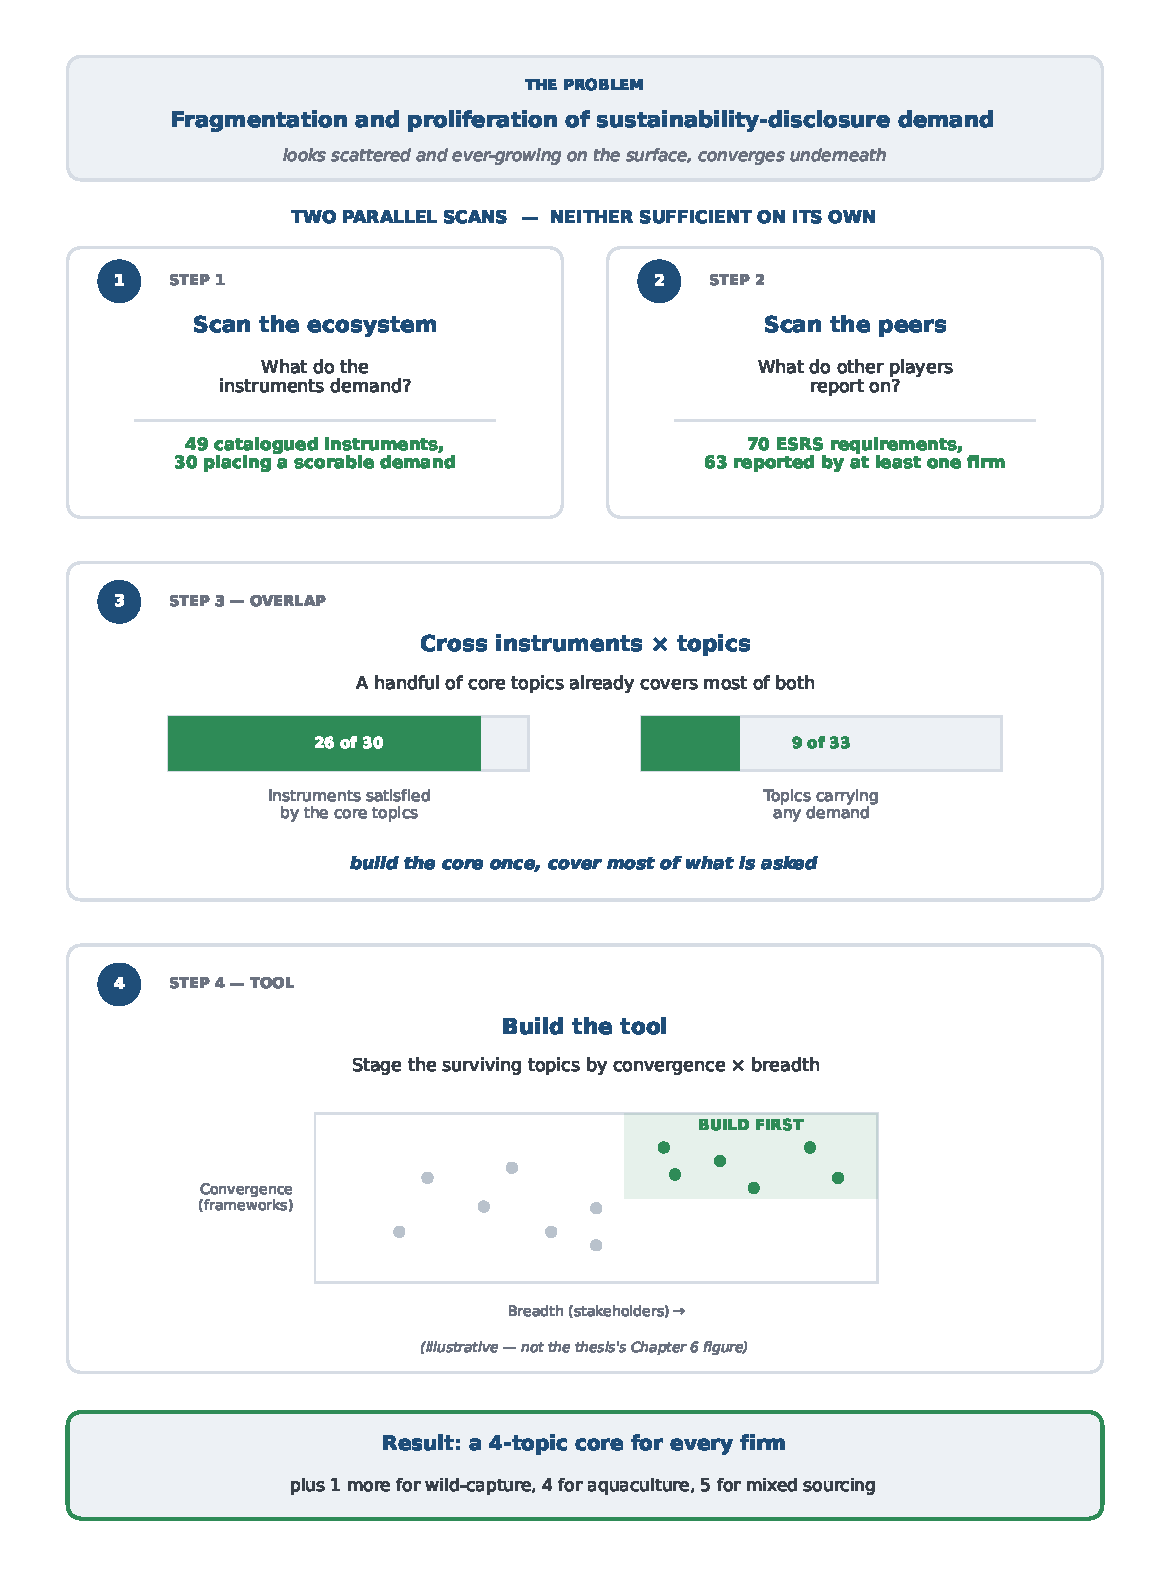
\includegraphics[width=0.82\linewidth]{methodology_diagram_corrected.pdf}
\caption{The thesis's four-step methodology, answering RQ1--RQ3 above:
Step~1 scans the disclosure ecosystem (Chapter~4, RQ1), Step~2 scans the
cohort frontier (Chapter~5, RQ2), and Steps~3 and~4 - crossing the two
to find where demand converges, then building the diagnostic tool on
that finding - are carried out together in Chapter~6 (RQ3). Neither scan is
actionable on its own: the ecosystem scan returns 49 catalogued instruments and
the cohort scan 70 disclosure requirements, and it is their intersection rather
than either list that yields a workable set of priorities. Chapters
5--7 each return to this figure as their starting point.}
\label{fig:methodology-overview}
\end{figure}
\FloatBarrier

\subsection{3.2 Intended contributions}\label{intended-contributions}

The thesis contributes to three audiences:

\begin{itemize}
\item
  \textbf{For seafood SMEs:} the thesis delivers a diagnostic framework
  and a prioritised, sequenced set of build-first disclosure topics - and
  the datapoints beneath them - tailored to the firm's own mix of
  demands, intended as a basis for strategic discussion within the firm
  rather than a compliance checklist.
\item
  \textbf{For EU policy:} it offers empirical input to the ongoing
  simplification debate (Omnibus, VSME extension, sector standards
  postponement). The cross-stakeholder hotspot analysis identifies where
  the regulatory and voluntary disclosure ecosystem is converging and
  therefore where coordination or capping of demand would deliver
  disproportionate burden reduction for SMEs. This aligns with the
  Competitiveness Compass target of cutting administrative burden by
  $\geq$35\% for SMEs (European Commission, 2025).
\item
  \textbf{For academia:} it provides a first systematic mapping of
  cross-stakeholder disclosure demand at the sector level using a defined
  coverage scale, extends the sustainability-reporting maturity-model
  literature by operationalising it as a diagnostic tool, and applies the
  reactive/proactive CSR distinction to empirical material.
\end{itemize}

\subsection{3.3 Research design}\label{methodology}

\textbf{Organisation of the thesis, and its reasoning.} The thesis integrates
its methodology and its results rather than presenting them in separate
chapters, because the four steps use different data and different methods.
\emph{Each of the three empirical chapters is therefore self-contained}: Chapters~4, 5 and~6 each open with
the reasoning behind their step, set out their own data and coding procedure,
report their own findings, and close by interpreting what those findings do and
do not establish. Chapter~6 carries two steps rather than one, because
locating convergence and building the diagnostic on it are drawn from the same
matrix.

This structure is deliberate. A pooled methodology chapter would have to
describe three unrelated procedures in the abstract, before the reader knows what
any of them is for, and a pooled results chapter would then separate each finding
from the method that produced it. Keeping them together makes each step
independently auditable.

What remains genuinely shared is presented in the remainder of this section: the
common measurement framework, the cohort, the data and coding procedures, and the
validation strategy. Chapter~7 then draws the three sets of findings together, reads them
against the conceptual framework of Chapter~2, and states the limitations that
apply across all of them.

\textbf{A common reference frame.} To compare and aggregate demand across a
fragmented field of instruments, the analysis adopts the European Sustainability
Reporting Standards (ESRS) as a common coordinate system - the most comprehensive
and legally anchored topic structure available, its ten topical standards (E1--E5,
S1--S4, G1) resolving into a defined set of disclosure requirements. Instruments and
reports written to other frameworks are read onto this structure, so that every
demand and every disclosure is expressed in one vocabulary. The choice, and its
limits, are developed where the frame is first used (Chapter~4 for the instrument
landscape, Chapter~5 for the cohort).

\textbf{Cohort and case selection.} The empirical work centres on six large
European seafood processors, selected purposively as among the sector's most advanced
sustainability reporters - not as a representative sample but as an upper-bound
proxy for what the sector can currently disclose. The selection spans the main
sourcing models so that the disclosure pattern is not an artefact of a single
production system; the full rationale and the cohort table are given in Chapter~5.

\textbf{Data and coding.} The analysis rests on two hand-built, hand-coded datasets:
the cohort firms' most recent sustainability reports, coded at
disclosure-requirement level against the ESRS structure (Chapter~5); and a catalogue
of the regulatory, customer, investor and industry instruments active in the sector,
each coded for the demand it places on each disclosure topic (Chapters~4 and~6).
Coding was performed manually from primary documents and cross-checked against the
underlying datapoints; the per-cell coding protocol is set out in Chapter~6.

\textbf{Validation.}\label{framework-validation-strategy} The framework rests on
three legs that do not depend on outside confirmation. Its construction is grounded
in the theory of Chapter~2 and in primary regulatory and standard-setting documents.
Its coding is checked for consistency against defined datapoints and logged
cell by cell. And it is applied to a worked case (Chapter~6) to show that it
yields a usable prioritisation.

A fourth leg is external and, at the time of writing, incomplete. The instrument
classification of Chapter~4 was discussed with industry contacts at Seafood Europe
during its construction, and the completed classification and cohort coding have
been submitted to the sustainability leads at the six cohort firms for review. This
is member checking (Lincoln \& Guba, 1985): a corroborating step, not a formal
reliability test. Any corrections it returns will be incorporated before final
submission, and the analysis does not depend on it. Practitioner validation of the
worked case with a firm itself is left to future work.



% Counter baseline before the angle chapters. Originally a defensive reset,
% because the archived \iffalse blocks were still stepping the counters.
% Those blocks were deleted on 2026-08-07; these two lines are kept because
% the numbering was verified identical with them in place (figure 1 accounts
% for fig:methodology-overview in Section 2.1, which precedes this point).
% Do not remove without rebuilding and checking figure/table numbers.
\setcounter{table}{0}
\setcounter{figure}{1}

%% ===================================================================
%% MODULAR ANGLE CHAPTERS (wired in)
%% ===================================================================
% =====================================================================
% STEP 1 — THE DISCLOSURE ECOSYSTEM  (rewrite v2, per Ruben's comments)
% Scope: this chapter is ONLY the construction of the necessity-domain
% matrix (screening + the classifying framework) and simple counts +
% the matrix figure. All scoring (what each instrument demands topic by
% topic, opt-in mechanics, sparse-matrix, narrow-law/broad-cascade) moves
% to Steps 3-4 (Ch 7).
% Counts verified against Necessity_Domain_Matrix_v8.xlsx.
%   Chapter presents the FULL landscape (all 49 catalogued); winnowing to the
%   30 scored is deferred to Steps 3-4 (Ch 7), per Ruben.
%   Full-landscape (VSME=Customer): Tiers 19/10/11/9; Domain 19 seafood / 30 general;
%   Source Regulator 19, Customer 14, Investor 6, Industry/NGO 10.  Scored subset = 30.
% =====================================================================

\section{5. The disclosure ecosystem}\label{angle1-ecosystem}

The first step scans the \emph{ecosystem}: it establishes which sustainability
instruments act on a European seafood-processing SME, and classifies each by how
obligatory it is and which stakeholder drives it. In doing so it constructs the
first component of the study's central instrument - the demand matrix - by
fixing and ordering its columns. This chapter does not yet ask \emph{what} each
instrument demands, topic by topic; that scoring, and the convergence it reveals,
is the work of Chapter~7. Here the question is prior and structural, and it is the thesis's first: who asks, and
how bindingly? This is Step~1 of the methodology set out in
Figure~\ref{fig:methodology-overview}.

\subsection{5.1 Constructing the necessity--domain
map}\label{ecosystem-construction}

\textbf{Identifying the instruments.} The instrument set was assembled in three
steps. First, candidate instruments were identified from two complementary
sources: the sustainability reports of the six large seafood processors that form
this study's cohort (Chapter~6), which show the regulations, certifications and
frameworks that leading firms in the sector actually respond to; and a structured
scan of EU sustainability law and the principal voluntary standards, ratings and
initiatives active in the sector. Second, each candidate was screened against two
inclusion gates: that it bears on an environmental, social or governance matter
(excluding purely fiscal, customs and data-protection law), and that it places a
binding obligation on the \emph{organisation itself} - a disclosure,
due-diligence, certification or market-access requirement - rather than merely
binding Member States or granting an individual employee an entitlement. Third,
the classification was built against how the demands are experienced in practice
rather than against formal legal status alone. Industry contacts at Seafood Europe
were consulted on the necessity ranking while it was being drawn up, and the
completed classification has been submitted to the cohort firms for review
(Chapter~4, \nameref{framework-validation-strategy}).

\textbf{A status for each instrument.} The catalogue deliberately keeps the
\emph{whole} field in view: every instrument that acts on the sector is placed in
the map, whether or not it ultimately enters the scored analysis. Each therefore
carries a status alongside its tier, domain, source and locus - the four
classifying attributes introduced below. An instrument is \emph{scored}; held out
as the CSRD/ESRS \emph{baseline} reference; set aside as \emph{context}, binding
Member States rather than the processor, as the Common Fisheries Policy does; or
\emph{excluded} for failing a screening gate, as a purely fiscal law does, or a
benchmark that rates other schemes rather than demanding anything of the
processor.

\textbf{The necessity axis: four tiers.} The framework's spine ranks each
instrument by how imperative it is from the SME's own perspective, on a gradient
of obligation that runs from \emph{coercive}, legally enforced requirements at the
base to \emph{normative}, voluntary commitments at the top - the institutional
gradient developed in Chapter~3 (DiMaggio \& Powell, 1983; Suchman, 1995). The
four tiers make it operational, each a point on that gradient:

\begin{itemize}
\item \textbf{Tier~1 - legal licence to operate.} Binding law, without which
the firm cannot lawfully trade: the IUU and Fisheries Control Regulations,
packaging law, occupational-safety law - coercive obligation in its purest form.

\item \textbf{Tier~2 - market licence to operate.} Legally optional but
commercially non-negotiable: a recognised certification or social audit - MSC, ASC, SMETA and EcoVadis are the most common examples in this sector,
not an exhaustive list - without which a major retail or foodservice
customer will not list a supplier. US Foods, for instance, requires any
GSSI-benchmarked certification (MSC or BAP are given only as examples) for
its top supplier tier and reserves the right to end a supplier relationship
over unresolved non-compliance (US Foods Holding Corp., 2025); several major
retailers make MSC or ASC specifically a sourcing-policy condition (Blank,
2025). The obligation is enforced by the market rather than the state, and
which specific scheme satisfies it varies by buyer and species.

\item \textbf{Tier~3 - competitive expectation.} Increasingly normalised
reporting frameworks whose absence is a competitive disadvantage - the VSME,
GRI, and the value-chain disclosures cascaded from customers under CSRD. This is
the mimetic-normative middle, where firms adopt what peers and buyers expect.

\item \textbf{Tier~4 - strategic differentiation.} Genuinely voluntary
commitments that signal leadership (SBTi, the UN Global Compact, TNFD). Adoption
is elective and reputational.
\end{itemize}

The tiers rank the \emph{instruments} by how binding each is; they do not by
themselves say which \emph{topics} a firm should build first. A firm that answers
only the binding tiers as each demand lands is reactive; the proactive move
(Sharma \& Vredenburg, 1998; Torugsa et al., 2013; the distinction developed in
Chapter~3) is to build, ahead of demand, the shared datapoints that recur across
many instruments regardless of tier, determined instead by how far demand
\emph{converges} across the ecosystem, how many stakeholder channels ask for a
topic, not by tier position.

\textbf{The domain axis.} Cutting across the tiers, the domain axis separates
\emph{seafood-sector-specific} instruments (the fisheries and aquaculture
regulations and certifications, and the GDST traceability standard) from
\emph{general corporate-sustainability} instruments that apply to the processor as
an enterprise like any other (climate, packaging, labour and governance law and
the cross-sector reporting frameworks).

\textbf{Two attributes: source and obligation locus.} Each in-scope instrument
carries two further tags. Its \emph{source} is the stakeholder whose demand the
processor actually answers, assigned by a single test - does the instrument
legally bind the processor? Where it does, the source is the \emph{regulator} (the
Fisheries Control Regulation binds the processor directly). Where it does not, the
source is the stakeholder that transmits the demand: a retailer-required
certification such as MSC codes to \emph{customer}; a capital-market standard such
as SFDR to \emph{investor}; an NGO-led framework such as GDST to
\emph{industry/NGO}. This test deliberately reassigns instruments whose nominal
issuer is a regulator to the channel through which a sub-threshold SME actually
meets them: CSRD and CSDDD, written for large undertakings, reach the small
processor not as law it must obey but as data its large customers must extract
from it, and so code to \emph{customer}. The same reasoning codes the VSME to the
customer channel: although a voluntary standard, in practice a small seafood
processor adopts it to answer a large customer's value-chain request rather than
to address capital markets. This does partly double-count the ESRS content that
also reaches the firm through CSDDD - a limitation accepted here because, for
seafood processors specifically, that demand genuinely arrives through the
customer channel.

The \emph{obligation locus} records, separately from source, whether the
processor is itself the bound party: \emph{direct} where the processor is the
obligated, certified or reporting entity (a processor holding MSC
chain-of-custody certification, which it maintains and is audited against);
\emph{indirect} where the obligation sits elsewhere and reaches the processor
through a buyer's demand or its own disclosure duty (CSDDD, which binds the large
customer and arrives as a value-chain questionnaire); and \emph{context} where
the instrument binds a Member State or another actor with no mechanism that
transmits an obligation to the processor at all (the Common Fisheries Policy).
Holding source and locus apart prevents the common error of reading the legally
bound party off the identity of the actor who actually applies the pressure.

\textbf{Two caveats on the map.} First, the instrument set is calibrated to
leading firms: it was screened from the reports of six large processors, so it
captures what mature, well-resourced firms respond to. It may therefore both
include instruments a small SME does not yet face and understate informal or
local demands it does. Second, necessity is profile-dependent. The tiering
assumes the modelled SME - a business-to-business supplier selling to large EU
retailers and exporting - for which retailer certifications are a genuine
market licence; a firm selling locally or direct to consumers would re-tier
several instruments.

\subsection{5.2 The instrument landscape}\label{ecosystem-landscape}

The catalogue comprises \textbf{49 instruments}
(Figure~\ref{fig:necessity-domain}) - the full field acting on a European
seafood processor. Read as counts, the landscape has three features.

By \emph{necessity tier}, it is weighted toward the binding base: 19 instruments
sit at Tier~1 (legal licence to operate), 10 at Tier~2 (market licence), 11 at
Tier~3 (competitive expectation) and 9 at Tier~4 (strategic differentiation). The
mandatory legal floor is the single largest block.

By \emph{stakeholder source}, regulators account for 19 instruments and customers
for 14 - together two-thirds of the field - while investors (6) and industry
or NGO initiatives (10) make up the remainder. What a small processor faces is
thus overwhelmingly a regulator-and-customer affair.

By \emph{domain}, 19 instruments are seafood-sector-specific - the fisheries and
aquaculture regulations and certifications together with the GDST traceability
standard - and 30 are general corporate-sustainability instruments. Most of what
acts on a seafood processor is not peculiar to seafood at all.

Of these 49, thirty enter the scored demand matrix in Chapter~7; the remainder
are held out as the CSRD/ESRS baseline, set aside as context because they bind
Member States rather than the processor, or excluded for failing a screening
gate. Every instrument named here is defined in full - the organisation behind
it, its legal reference, current status and official source - in the
\nameref{app:glossary}.

\begin{figure}[ht]
\centering
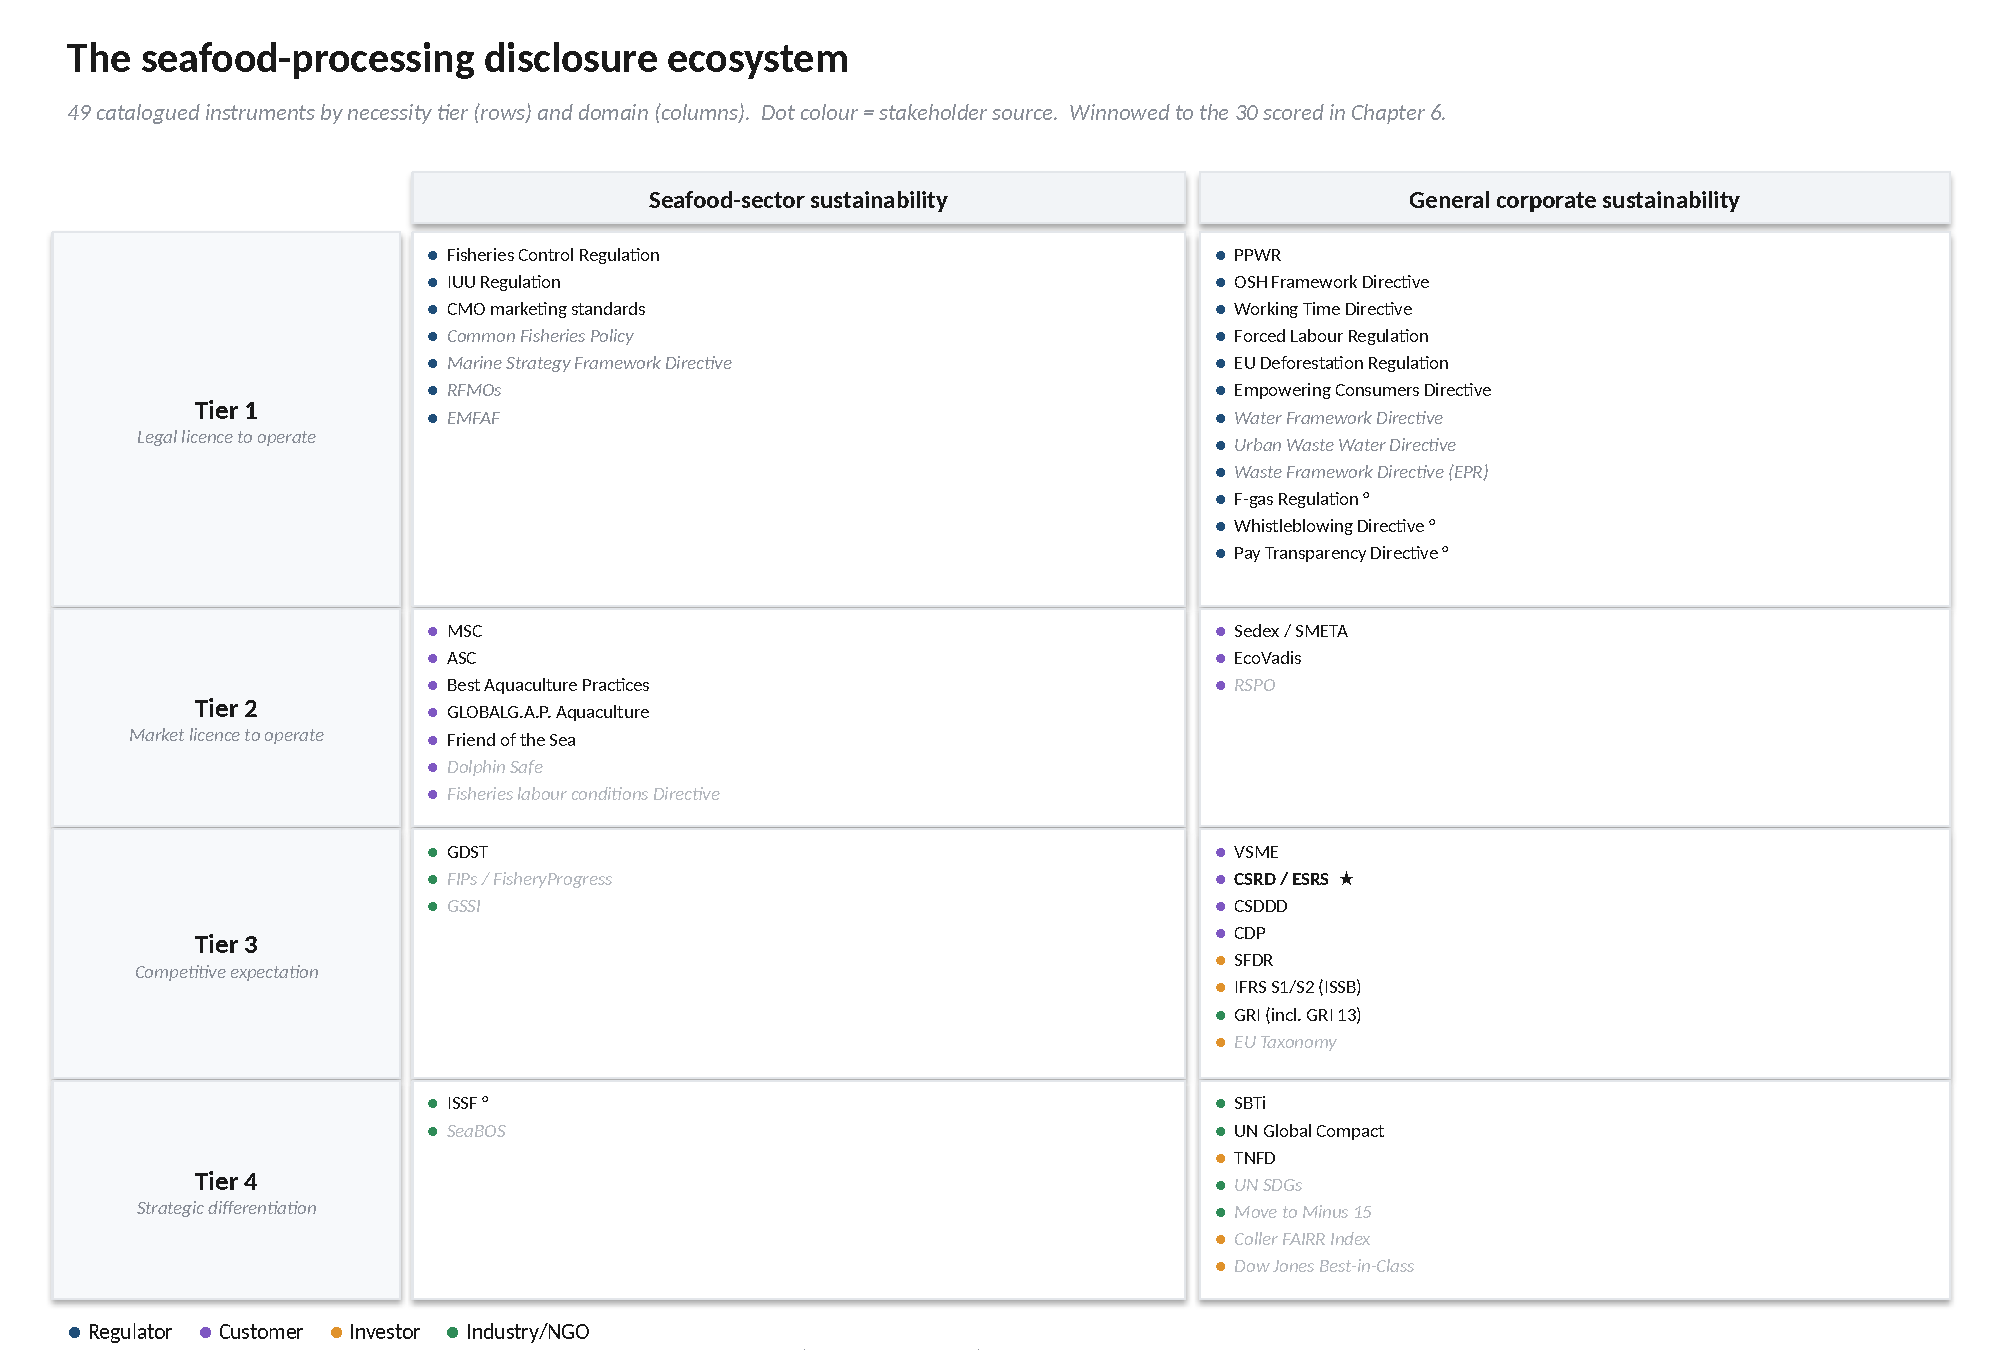
\includegraphics[width=\linewidth]{necessity_domain_matrix.pdf}
\caption{The seafood-processing disclosure ecosystem: all 49 catalogued
instruments arranged by necessity tier (rows) and domain (columns). Dot colour
marks the stakeholder source; text style marks status - normal = scored,
``\,\textdegree\,'' = firm-profile opt-in, $\star$~= the CSRD/ESRS baseline, grey
italic = context (binds Member States, not the processor), pale = excluded. The
winnowing to the 30 scored instruments is set out in Chapter~7. A full reference
entry for each instrument - the body behind it, its legal reference, status and
official source - is given in the \nameref{app:glossary}.}
\label{fig:necessity-domain}
\end{figure}

This map fixes the columns of the demand matrix: who asks, and how bindingly. What
each instrument actually demands, topic by topic, and where those demands
converge into build-first priorities, is taken up in Chapter~7. First, however,
Chapter~6 turns to the rows - establishing, from the disclosures of the sector's
most advanced reporters, what a mature seafood firm actually reports.

\FloatBarrier
% =====================================================================
% ANGLE 2 - THE COHORT FRONTIER  (self-contained draft for review)
% = existing "seafood disclosure frontier" chapter from main.tex,
%   PLUS a new theory framing (disclosure maturity + institutional convergence).
% =====================================================================
\section{5. The seafood disclosure frontier: evidence from six large
reporters}\label{cohort-analysis}

This chapter answers the thesis's second research question: \emph{what do mature
European seafood processors actually disclose?} It establishes that practice from
primary documents, setting the assumed \emph{upper bound} of sector disclosure
depth. Both the demand mapping that follows and the expectations placed on
smaller firms should be read against it. The cohort is not
a picture of typical practice; it is a picture of the best-in-class frontier.
This is Step~2 of the methodology set out in
Figure~\ref{fig:methodology-overview}.

\textbf{Scope note: this is a coverage analysis, not a judgement of reporting
quality.} It measures whether a topic is disclosed at all, coded from each
firm's own published sustainability report or ESRS-index appendix, using
only public information - no non-public data, site visits or firm-specific
verification. A firm scoring lower may simply have a different production
system, framework, or reporting year, not weaker sustainability performance;
no ranking or evaluative claim about the six companies is intended.

\FloatBarrier
\subsection{5.1 The frontier as a disclosure-maturity
question}\label{cohort-theory}

Corporate sustainability disclosure is not adopted all at once but develops
through stages of organisational maturity: firms move from ad-hoc, reactive
reporting toward systematic, integrated disclosure as capability accumulates
(Baumgartner \& Ebner, 2010),
and the completeness and quality of a firm's
reporting can be read as a position on that maturity gradient (C\"oster et al.,
2020).
The most advanced reporters in a sector therefore mark its practical
\emph{frontier}: the upper bound of what is currently feasible - and relevant to
seafood processing - to disclose given real data systems and resources. This research therefore treats the frontier as a ceiling that resource-constrained
SMEs can grow into, not one they can replicate today.

Two features make that frontier analytically useful here. First, when processors
as different as a vertically integrated salmon operation and a pure whitefish
processor nonetheless disclose the same handful of topics, that agreement is
unlikely to be coincidence. It reflects a shared expectation - what the sector
has collectively come to treat as standard practice for a credible reporter -
rather than each firm's independent choice; institutional theory calls this the
mimetic and normative pressure that makes practices converge across an industry
(DiMaggio \& Powell, 1983). This is an interpretive reading, and a competing one
is possible: firms may converge because the same topics carry the greatest
reputational risk, or simply because they are the easiest to report. That each
firm's disclosures are anchored in its own double-materiality assessment is a
partial check against pure convenience, though not a decisive one. Read either
way, a universal core is the sector's \emph{revealed} consensus on what a serious
reporter covers - what counts as complete disclosure in practice, not just a
coincidental overlap between six firms' independent choices.
Second, the frontier calibrates the realistic ambition for a
resource-constrained firm: if even the best-resourced reporters leave requirements
uncovered, completeness is the wrong yardstick for an SME, and the question
becomes which subset of disclosures matters most - the question the demand
mapping in the following chapter takes up.

Existing work characterises sustainability-reporting maturity in general terms
(Baumgartner \& Ebner, 2010) and describes seafood
sustainability governance at the level of the movement and its institutions (Bush
\& Oosterveer, 2019; Barclay \& Miller, 2018), but does not map, at
disclosure-requirement level, what the sector's leading firms actually report.
This chapter supplies that map and reads it for three things: how \emph{much} the
leading firms disclose (the height of the frontier), which topics \emph{every}
firm reports (the universal core), and which relevant topics \emph{none} of them
report (the sector's collective gaps).


\FloatBarrier
\subsection{5.2 The cohort and case selection}\label{cohort-selection}

Six large seafood processors were selected purposively as among the most
advanced sustainability reporters in the sector rather than as a
representative sample. The selection deliberately spans the sector's main
sourcing models, so that the disclosure pattern that emerges cannot be an
artefact of a single production system: wild-capture tuna (Thai Union,
Bolton), aquaculture salmon (Mowi), an integrated wild-plus-aquaculture
operation (Profand), and pure processing/branded firms whose variation comes
from the species and origins they source rather than from a distinct
production system of their own (Nomad Foods, Espersen).
All six are seafood \emph{processors}, but they differ in how far they integrate
upstream - from Mowi, which farms its own salmon and mills its own feed, to
Espersen, a near-pure whitefish processor. This matters for reading the
reports: Mowi discloses feed and farming as its \emph{own} operations,
while Espersen meets the same topics only as \emph{sourcing} questions about
its suppliers - the two are not directly comparable without accounting for
this difference.

The six were chosen on three criteria: they are among the largest seafood
processors by turnover; each publishes a full, structured sustainability report
under the ESRS or the GRI Standards; and together they span its main sourcing
models.

The second criterion carries most of the weight, and it is worth being precise
about what it does and does not establish. ``Most advanced'' here is a sampling
frame rather than a measured rank. Of the roughly 3{,}245 EU enterprises that
process fish as their main activity, about two-thirds are micro-enterprises and
only some two per cent employ 250 people or more (STECF, 2025). The
overwhelming majority therefore sit
below the CSRD reporting thresholds and face no obligation to publish a
structured sustainability report at all. Publishing one regardless is itself the
distinguishing act, and the six are drawn from the small population that does. No claim is made that they are the six \emph{best} reporters in the sector,
only that they sit inside the set that reports at all and, within it, span the
sourcing models and the size range.

Whether firms selected this way are advanced in absolute terms is a separate
question, and one this chapter's own results answer rather than assume. They are
not complete: the deepest reporter covers 60 of the 70 topical requirements and
the shallowest 33, and seven requirements are reported by no firm in the cohort
(Sections~5.4 and~5.6). The frontier they mark is therefore a realistic ceiling
rather than a standard of completeness - which is precisely why it is a usable
benchmark for a smaller firm.

The aim of the selection is therefore not representativeness but reach: to
assemble the firms most likely to have pushed disclosure to its current limit, so
that the pattern common to \emph{them} marks the sector's realistic ceiling.
By 2024 turnover the six span more than a tenfold range: Mowi (EUR~5.6bn) and
Thai Union (THB~138.4bn, approx. US\$4.0bn / EUR~3.6bn) are the largest, followed
by Bolton Group (EUR~3.5bn group-wide, of which approx. EUR~2.4bn is its food
division) and Nomad Foods (EUR~3.1bn), with Profand (approx. EUR~1.1bn) and
Espersen (DKK~3.3bn, approx. EUR~440m) smaller but still among the sector's
largest specialist processors.\footnote{2024 group turnover, most recent
published results, converted to EUR at approximate contemporaneous rates where
the firm did not report in EUR: Thai Union (\emph{Thai Union FY2024 press
release}, thaiunion.com); Mowi (\emph{Mowi Q4 2024 Report}, mowi.com); Bolton
Group (Undercurrent News, ``Tuna sales boost Bolton's turnover, profit in
2024,'' Aug.\ 2025); Nomad Foods (Q4/FY2024 earnings release, nomadfoods.com);
Profand (Undercurrent News, ``Spain's Profand surpasses EUR1bn revenue in
2024,'' Apr.\ 2025); Espersen (Undercurrent News / SeafoodSource coverage of
FY2024 results). Four of the six - Bolton, Mowi, Nomad Foods and Thai Union - also appear among Mordor Intelligence's top-ranked players in the European
seafood market (mordorintelligence.com/industry-reports/europe-seafood-market/companies);
that source does not cover Profand or Espersen, so cohort-wide ranking evidence
is partial rather than complete.} The selection also gives geographical
spread across the sector's main European processing regions - from southern
Europe (Bolton in Italy, Profand in Spain) to the Nordics (Espersen in
Denmark, Mowi in Norway) and the UK (Nomad Foods) - with Thai Union added
as one of the largest seafood processors supplying the EU market from
outside it, extending the cohort's reach beyond Europe without abandoning
the EU-market focus.
Table~\ref{tab:cohort-r} summarises the cohort.
\begin{table}[H]
\centering
\caption{Cohort overview and reporting coverage. Coverage is reported
disclosure requirements (DRs) as a share of the 70 topical ESRS disclosure
requirements (E1--E5, S1--S4, G1); see the Section~5.3 section.}
\label{tab:cohort-r}

\footnotesize
\begin{tabularx}{\textwidth}{@{} l l X X c c @{}}
\toprule
\textbf{Company} & \textbf{HQ} & \textbf{Sourcing model} & \textbf{Reporting basis} &
\textbf{DRs} & \textbf{Coverage} \\
\midrule
Thai Union  & Thailand & Wild-capture tuna & GRI, in accordance & 60 & 86\% \\
Nomad Foods & UK       & Multi-species     & GRI, with reference & 52 & 74\% \\
Bolton      & Italy    & Wild-capture tuna & ESRS            & 45 & 64\% \\
Profand     & Spain    & Wild + aquaculture & CSRD double materiality; GRI supporting & 43 & 61\% \\
Espersen    & Denmark  & Multi-species     & ESRS            & 34 & 49\% \\
Mowi        & Norway   & Salmon aquaculture & ESRS           & 33 & 47\% \\
\bottomrule
\end{tabularx}
\end{table}

Turnover and coverage do not track each other within the cohort: Mowi, the
largest firm by 2024 turnover, reports the fewest requirements of the six
(47\%), while the smaller Profand and Nomad Foods both report more. Firm size
is therefore not read here as a driver of reporting depth; what varies across
the six is each firm's own reporting maturity and sourcing model, not the
resources it commands.

The six also differ sharply in structure, and it is worth stating why they remain
comparable. Mowi is a vertically integrated aquaculture producer; Thai Union
depends heavily on externally sourced raw material; Profand combines fishing,
aquaculture, processing and commercialisation in one group. Those differences
shape both which topics each firm's double-materiality assessment returns as
material and how deeply it is expected to report on them. Three features of the
design absorb that. First, the denominator is external and identical for all six:
the 70 topical ESRS disclosure requirements, not a cohort-derived list, so no firm
is scored against another's materiality assessment. Second, the measure is
breadth at requirement level - whether a topic is addressed at all, a question
that can be put to any business model - rather than depth or quality. Third, and
most important, the load-bearing result of this chapter is not the per-firm figure
but the set of requirements reported by all six. Structural difference makes that
intersection harder to reach, so agreement across six unlike firms is stronger
evidence of a genuine sector core than agreement across six similar ones would be.
Where the differences do bite is on the individual coverage figures, which is one
reason the chapter draws no ranking from them.

One feature of the cohort must be stated plainly at the outset, because it bounds
every claim that follows: the cohort is a purposive \emph{upper-bound} sample. It
is taken as a proxy for what is feasible and important to disclose in this sector - an
assumption the robustness checks below probe - not for what a typical firm does,
and no inference about average practice is drawn from it. How the six firms'
disclosures, reported under two different frameworks, were placed on a single
comparable measure is set out next.

\FloatBarrier
\subsection{5.3 Data and method}\label{cohort-method}

\textbf{The ESRS as the common ruler.} The measure is built on the European
Sustainability Reporting Standards (ESRS), the disclosure taxonomy that
operationalises the EU's Corporate Sustainability Reporting Directive. The ESRS
are used here not because every cohort firm reports under them - three do not -
but because they are the most comprehensive and legally anchored topic structure
available. Ten topical standards (E1--E5, S1--S4, G1)\footnote{E1 Climate
change; E2 Pollution; E3 Water and marine resources; E4 Biodiversity and
ecosystems; E5 Resource use and circular economy; S1 Own workforce; S2
Workers in the value chain; S3 Affected communities; S4 Consumers and
end-users; G1 Business conduct.} resolve into a defined, published set of
disclosure requirements. That fixed structure gives one stable ruler onto which
disclosures written under any framework can be placed and compared. It is what
makes a cross-firm comparison - and, in later chapters, a cross-instrument
one - possible at all. Coverage in this chapter is
therefore always \emph{ESRS-aligned coverage in practice}, never a judgement of
legal ESRS compliance. As the standard mandatory for CSRD-scoped firms and the
most complete public sustainability taxonomy in force, the ESRS is also the
natural benchmark: even under the Omnibus simplification it remains the reference
against which other frameworks - including the VSME and, through the
interoperability mapping used below, the GRI - are aligned (Hummel \& Jobst,
2024).

\textbf{Data and scope.} The primary sources are the firms' own published
sustainability reports: the most recent report for each firm, from financial
year~2024 and, where already published, 2025 (the exploratory year-over-year comparison later in the chapter
uses the three firms for which both are available), supplemented
where available by each firm's CSRD-aligned ESRS-index appendix. Coding proceeds
from each report's own framework index - the ESRS index appendix for the three
ESRS reporters, the GRI content index for the three GRI reporters - rather than
from a full reading of the report body. Each indexed disclosure was coded against
the \emph{topical} ESRS standards - the ten environmental, social and governance
standards (E1--E5, S1--S4, G1) and their
disclosure requirements. The two cross-cutting standards, ESRS~1 and ESRS~2
(general principles and general disclosures), are deliberately out of scope: they
govern \emph{how} a firm reports rather than \emph{which} sustainability topics it
addresses, and it is topical coverage that this chapter measures.

\textbf{Unit of analysis: material topics, not IROs.} Coding is at the level of
the ESRS topical \emph{disclosure requirements} (DRs) - the material
sustainability topics a report addresses - and deliberately not at the level of
the firm-specific impacts, risks and opportunities (IROs) that sit beneath a
double-materiality assessment. Three reasons make the DR the right grain. First,
IROs are entity-specific by design: under ESRS~1 they are the output of each
undertaking's own double-materiality assessment, so one firm's impacts, risks and
opportunities are not defined on the same basis as another's and cannot be
aggregated into a cross-firm coverage measure. Second, the question here is one of
\emph{breadth} - which topics a mature reporter addresses at all - for which
presence at DR level is the natural unit; IROs speak to a firm's internal
prioritisation, not to the sector's disclosure frontier. Third, only three of the
six firms report under the ESRS, and the GRI reporters produce no ESRS-style IROs
at all, so the topical DR is the only common denominator on which all six firms
can be placed.

\textbf{Translating GRI to ESRS.} Only three firms report directly under the ESRS
(Mowi, Bolton, Espersen); the other three were coded through their GRI content
indexes, and those three sit at three different places on a spectrum. Thai Union
reports \emph{in accordance with} the GRI Standards, the fuller of the two GRI
application levels. Nomad Foods reports \emph{with reference to} them, citing
selected disclosures without claiming full application. Profand is a third case
again: its 2025 report is structured around a CSRD double-materiality assessment,
and GRI appears only as a supporting correspondence table appended to a document
whose primary architecture is the ESRS. Its GRI index is therefore a secondary
artefact rather than the report's organising spine - a distinction that matters
for what the coding can see, and one returned to below. A bridge was built to
score all six on one ruler. The bridge is the GRI-EFRAG interoperability index
(GRI \& EFRAG, 2024) applied in full: every GRI disclosure listed in that index was
carried across with the complete set of ESRS disclosure requirements EFRAG assigns
to it, including the cases where a single management-approach disclosure maps onto
requirements in more than one topical standard. Where the index states that a GRI
disclosure is addressed through the cross-cutting minimum disclosure requirements
(MDR-P, MDR-A, MDR-T) or as an entity-specific metric rather than through a named
topical requirement, no topical coverage was recorded. Sector-specific disclosures
drawn from GRI 13, for which EFRAG publishes no correspondence, were mapped by the
author and are identified as such in the bridge workbook. Three
rules governed that adjudication. Where the interoperability index records a full
correspondence, the mapping follows it directly. Where it records a partial one,
the GRI disclosure was accepted as evidence for the ESRS requirement only if it
addressed the requirement's substantive subject, not merely its topic area - so a
GRI water-withdrawal metric maps to E3-4 but not to the E3-1 water policy
requirement. Where one GRI disclosure spans several ESRS requirements it was
credited to each; where several GRI disclosures were needed to satisfy one, the
requirement was credited once. Every mapping decision is recorded with its source
clause in the bridge workbook, so the chain from a firm's index entry to a
coverage score can be reconstructed row by row. The
with-reference firms supply fewer mappable disclosures by construction, which is
one reason their coverage sits mid-range rather than at the top; it is a feature
of reporting choice, not of sustainability performance. Every firm's disclosures
therefore sit on the same ESRS structure regardless of native framework.

\textbf{What index-based coding measures, and what it misses.} Working from the
index rather than the report body is a deliberate choice with a known cost. The
benefit is reproducibility: the index is the firm's own declaration of what it
reports and where, it is applied identically to all six firms, and it is how a
customer's due-diligence team reads a report in practice. The cost is that a firm
whose index is selective scores below what its report body contains. That gap is
systematic rather than random. GRI 3-3, management of material topics, is the
disclosure carrying a firm's policies, actions and targets for each topic, and it
is the principal bridge to seven ESRS policy-and-action requirements - E1-2, E1-3,
E3-1, E4-2, E4-3, E5-1 and E5-3. It is optional for firms reporting \emph{with reference
to} the standards, and it is omitted entirely where the GRI table is a supporting
crosswalk rather than the report's primary index. Thai Union's index carries 27
GRI 3-3 entries and Nomad Foods' 16; Profand's carries none, in either reporting
year. The distinction is narrow but decisive: Profand does index GRI 3-1 and 3-2,
the process for determining material topics and the resulting list, in both 2024
and 2025. Those two disclosures map to ESRS 2, the general disclosures excluded
from scope above. Only GRI 3-3 carries the management approach - the policies,
actions and targets - and only GRI 3-3 bridges to the topical ESRS
policy requirements. Profand is
therefore coded as reporting none of those seven requirements, although its report
body describes a water-management policy aligned to ISO 46001, a biodiversity
policy applying the mitigation hierarchy, and 2030 circular-packaging targets. The
coding did not miss these; the index it was built from does not carry them.
Profand's figure of 39 requirements should be read as a floor.

\textbf{The ceiling the bridge imposes.} A second and distinct effect sits
alongside the first. Seven of the
70 topical disclosure requirements have no counterpart anywhere in the GRI-ESRS
interoperability index: E1-1, E1-8, E2-6, E3-5, E4-6,
E5-6 and G1-6. No GRI disclosure maps to any of them, so no
firm coded through a GRI index can score them however fully it reports. E1-1, the
climate transition plan, is the clearest case: Profand's report sets out a Net
Zero roadmap with 2035 and 2050 milestones, and the coding still records E1-1 as
absent - as it does for Thai Union and Nomad Foods, for the same structural
reason. Bolton and Mowi, both ESRS reporters, are the only firms in the cohort
recorded as reporting it. Where the first effect concerns how completely a firm
indexes its own disclosures, this one concerns what the bridge between two
frameworks can carry at all, and it applies uniformly to every GRI-coded firm.

The seven form a coherent set: the climate transition plan (E1-1), internal
carbon pricing (E1-8), payment practices (G1-6), and all four
anticipated-financial-effects requirements (E2-6, E3-5, E4-6, E5-6). These are
the forward-looking and financially quantified disclosures for which the GRI
Standards have no counterpart, so the gap reflects a genuine difference in what
the two frameworks ask rather than an artefact of the crosswalk.

Because the bridge cannot reach these seven, they were screened separately. For
each of the three GRI-indexed firms, and for both reporting years, the report body
was read directly for evidence of each of the seven requirements, with any finding
recorded against a page reference. The rule was fixed before the screening: where
the interoperability index provides no route to a requirement, coverage is
determined by direct reading of the report body. Only E1-1 was found. All three
firms disclose a climate transition plan - Thai Union's Path to Net Zero, Nomad
Foods' SBTi-validated targets and 2025 transition plan, and Profand's Net Zero 2050
roadmap - and E1-1 is coded accordingly for each, flagged in the workbook as
body-sourced rather than index-sourced. The remaining six were not found in any of
the six reports. Thai Union describes assessing a shadow carbon price but does not
operate one, which does not meet E1-8.

After that screening the ceiling no longer binds. Six of the seven are reported by
no firm in the cohort, on either instrument, so nothing is hidden behind them. The
seventh, E1-1, is now recorded for five of the six firms and enters the
near-universal set. The universal core of 13 is therefore exact rather than a
floor.

Both effects otherwise point the same way. Under-counting can only shrink the set
of requirements common to all six firms, so the convergence claim is not at risk.
What the two biases do distort is the firm-by-firm comparison in
Table~\ref{tab:cohort-r}, which is a further reason no ranking of the six is
intended.

The mapping and the DR-level coding both rest on analyst judgement. As a check on
that judgement, the coding has been submitted to the sustainability leads at the
cohort firms for review (Chapter~3, \nameref{framework-validation-strategy}). One
review has returned. Profand's sustainability lead identified eight disclosure
requirements substantively addressed in the report body but not reachable through
its GRI index; that exchange is the source of both limitations set out above, and
the coding was left unchanged so that the measure remains consistent across the
cohort. This corroborates the coding rather than
testing its reliability formally, and the analysis does not depend on it.

\textbf{Coding and consolidation.} Coverage is coded as binary presence or absence
at DR level: a firm scores~1 on a requirement where its reporting contains a
disclosure mapping to that requirement, and~0 otherwise. This measures
\emph{breadth}, not depth, quality or assurance - a requirement touched in a
single sentence and one reported exhaustively both score~1. The per-firm codings
were consolidated and analysed in a Jupyter notebook, which builds the
firm-by-requirement coverage matrix and the frequency distribution from which the
results in the following sections are drawn.

\textbf{The universe and the funnel.} The denominator is fixed and
externally defined, not cohort-derived: it is the full set of 70 topical ESRS
disclosure requirements - every DR across the ten topical standards (E1--E5,
S1--S4, G1) as set out in Commission Delegated Regulation (EU) 2023/2772
(European Commission, 2023), the ESRS Set 1 delegated act EFRAG's draft
standards were adopted into.
Beginning from this
complete set, rather than from what the cohort happens to report, is what lets the
coverage figures be read as a share of the whole relevant field. Applying the
coding produces a natural narrowing: of the 70 DRs, 63 are reported by at least
one firm (the remaining seven, reported by none, are examined in
Section~5.6),
28 by at least five of the six, and 13 by all six. This funnel is the
structure the results then read for the height of the frontier, its
universal core, and its gaps.
The per-standard version of this same frontier - what
is screened against what is actually covered - is shown directly below
(Figure~\ref{fig:p1-depth}).

\begin{figure}[htbp]
\centering
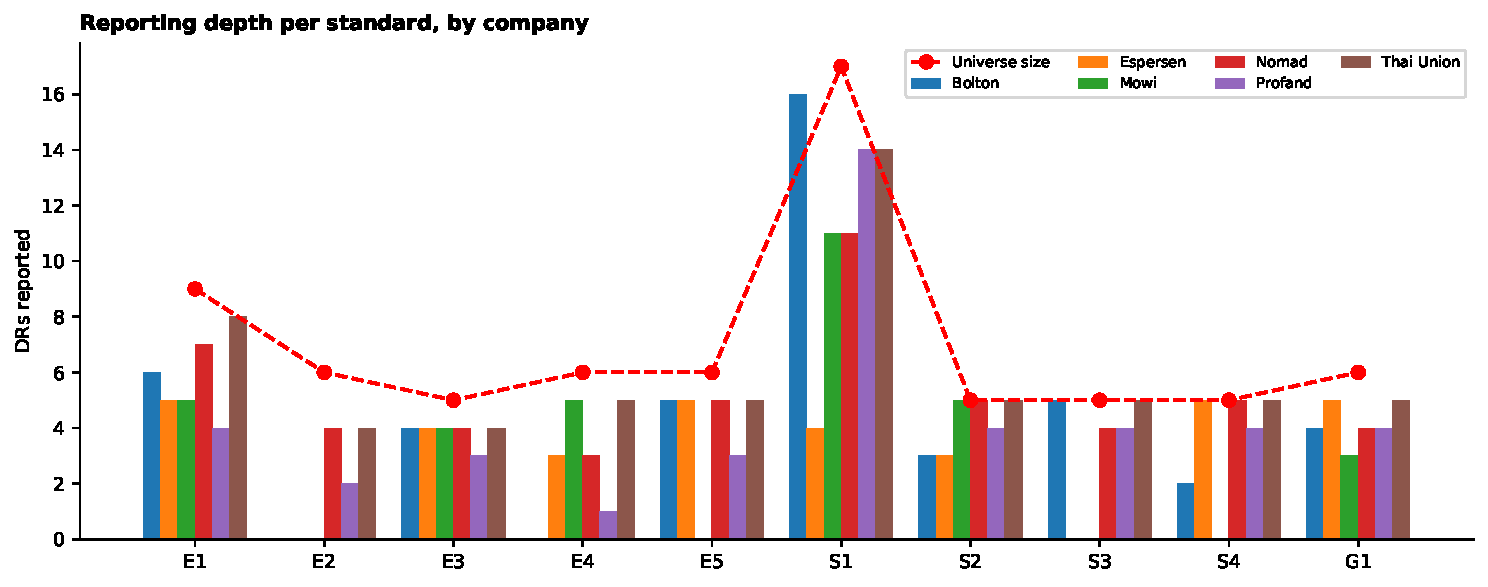
\includegraphics[width=\linewidth]{phase1/p1_depth_per_standard.pdf}
\caption{Reporting depth per topical standard, by company (bars), against
the number of screened DRs in each standard (red line). The gap between
the bars and the red line is widest for E2 (pollution) and E4
(biodiversity), the sector's thinnest topics.}
\label{fig:p1-depth}
\end{figure}

\textbf{What frequency does and does not mean.} One caveat governs the reading of
this funnel: it measures \emph{reporting convention} among large, mostly
CSRD-scoped reporters, not materiality for a small processor. A frequently
reported requirement is one an SME is likely to be \emph{asked about} as that
convention cascades down the value chain - a demand-relevance proxy - rather
than a topic asserted to be material for any individual firm. Whether these
revealed priorities fit a particular firm's situation is a separate question,
taken up in the cross-framework mapping and the worked case that follow.

\FloatBarrier
\subsection{5.4 The height of the frontier: a coverage
gradient}\label{cohort-gradient}

Coverage ranges from 33 to 60 of the 70 screened DRs
(Figure~\ref{fig:p1-heatmap}). Thai Union is the deepest reporter
at 60 DRs (86\%), followed by Nomad Foods (52; 74\%) and Bolton (45;
64\%); the median large reporter covers roughly 44 DRs, around 63\% of the
70-DR universe.
The immediate and consequential observation is that
\emph{even the frontier is incomplete}: the most advanced reporter in the sector
leaves around one relevant requirement in four uncovered (roughly 25 per cent),
and the median large reporter closer to two in five (around 40 per cent). If the
sector's most
resourced firms do not disclose the full set of relevant requirements, the
realistic ceiling for a resource-constrained SME sits well below
completeness - a point that reframes the SME question from 'how do we
report everything?' to 'which subset matters most?', which the demand
mapping in the following chapters answers.

The company-by-standard heatmap also shows that firms specialise: Bolton
reports most fully on own-workforce disclosure (S1, 16 of 17) and affected
communities (S3, 5 of 5); Espersen reports fewer S1 items (4 of 17) and no
S3 items in this coding, but is complete on consumers/end-users (S4, 5 of
5); Mowi's disclosure does not extend to affected communities (S3) or
consumers (S4) in this coding. The frontier is therefore not only
incomplete in height but uneven in shape from firm to firm.

\begin{figure}[htbp]
\centering
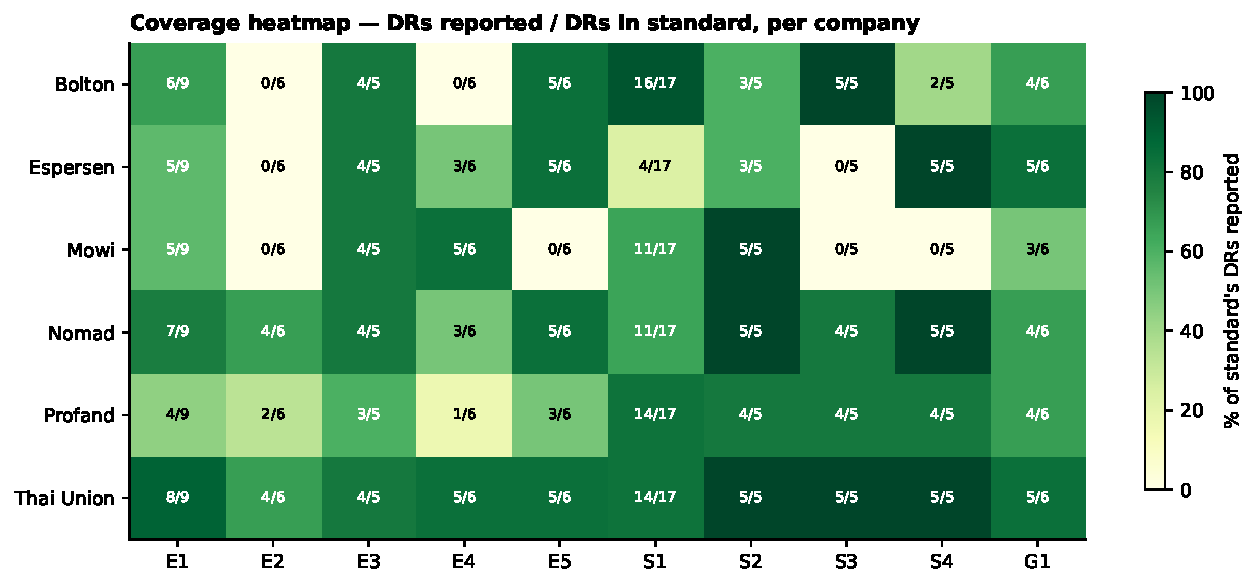
\includegraphics[width=\linewidth]{phase1/p1_heatmap.pdf}
\caption{Coverage heatmap: each cohort firm's reported DRs as a fraction
of the screened DRs in each of the ten topical standards (cell label
``reported / in standard''; shading is the percentage). Rows sum to each
firm's total in Table~\ref{tab:cohort-r}; the standard totals sum to the 70
screened DRs.}
\label{fig:p1-heatmap}
\end{figure}

\FloatBarrier
\subsection{5.5 The universal core: what every firm
reports}\label{cohort-core}

Beneath the gradient lies a stable core. Reading the universe by the
number of firms reporting each requirement produces a clean funnel: of the
63 DRs reported by at least one firm, 28 are reported by at least five, and
13 by \emph{all six} (Figure~\ref{fig:p1-frequency-r}). These 13 requirements are
the sector's empirically revealed \emph{baseline} - the disclosures every mature
reporter makes irrespective of sourcing model, and so, on the reading above, the
minimum a credible seafood reporter is now taken to be expected to cover. They
fall into four blocks:

\begin{itemize}
\item \textbf{Climate (3):} energy consumption and mix (E1-5), gross
  Scope~1--3 and total GHG emissions (E1-6), and climate targets (E1-4).
\item \textbf{Water (3):} actions and resources (E3-2), targets (E3-3),
  and water consumption (E3-4).
\item \textbf{Governance (2):} business-conduct policies and corporate
  culture (G1-1), and prevention and detection of corruption and bribery
  (G1-3).
\item \textbf{Social (5):} own-workforce policies (S1-1), workforce
  characteristics (S1-6), health-and-safety metrics (S1-14), and, for
  value-chain workers, policies (S2-1) and remediation channels (S2-3).
\end{itemize}

This narrowing is the core descriptive finding of the chapter: the sector
does not disclose evenly across a broad front, but converges onto a compact,
shared backbone.

One qualification bounds these two counts. Seven of the 70 requirements cannot be
reported by more than three firms, because the GRI-ESRS bridge offers no route to
them and half the cohort is coded through GRI indexes (Section~5.3). Six of those
seven are reported by no firm at all, so the qualification binds on a single
requirement: E1-1, the climate transition plan, which could in principle reach
five of six were all three GRI-indexed firms to disclose one. The core of 13 is
unaffected either way, since none of the seven could reach six of six.

\begin{figure}[htbp]
\centering
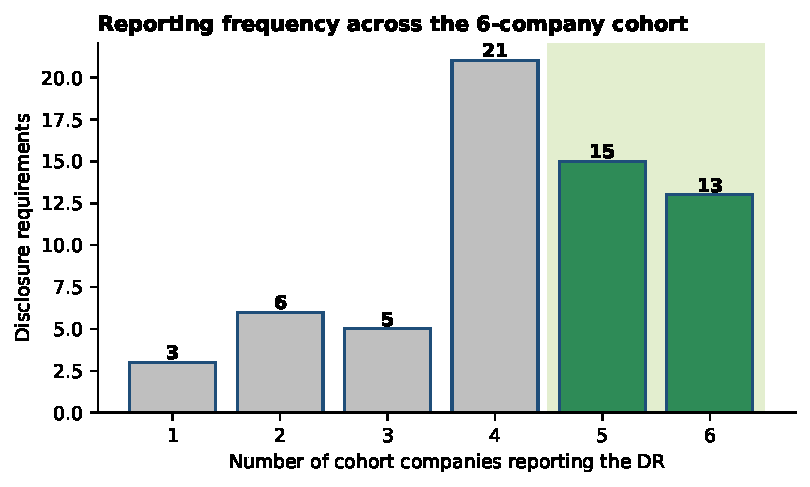
\includegraphics[width=0.8\linewidth]{phase1/p1_frequency.pdf}
\caption{Number of cohort firms reporting each DR, over the 63
requirements reported by at least one firm. The highlighted band (reported
by five or six firms) contains 28 requirements, of which 13 are reported
by all six - the universal core.}
\label{fig:p1-frequency-r} % RUBEN: overlaps fig:p1-frequency in Methodology 4.3 — same figure in both.
\end{figure}

\FloatBarrier
\subsection{5.6 The shape of the frontier: volume, consistency, and blind
spots}\label{cohort-shape}

Among the 63 reported requirements, disclosure is markedly social-heavy by
volume: 32 are Social, 26 Environmental, and 5 Governance, with the
own-workforce standard (S1) alone accounting for 17. This social weighting
holds within firms as well as across the universe: for every cohort
member, Social is the largest block of reported DRs and Governance the
smallest (Figure~\ref{fig:p1-esg}, panels~A--B). This is a volume comparison,
however, and the ESRS universe itself is uneven across pillars - 32 DRs each
for Environmental and Social, but only 6 for Governance. Normalized by each
pillar's own size (Figure~\ref{fig:p1-esg}, panel~C), Governance is in fact
the \emph{most} thoroughly covered pillar per firm on average (mean 69\% of
its 6 DRs, range 50--83\%, against a mean 56\% for Environmental and 70\% for
Social): the sector reports on a smaller
absolute footprint of governance topics not because it neglects them, but
because the ESRS asks fewer governance questions to begin with.

Volume, however, is not the same as consensus. Measuring each topic by the
mean number of firms reporting its requirements reveals where the sector
genuinely agrees (Figure~\ref{fig:p1-consistency}): consistency is highest for
water (E3, mean 5.75 of 6), value-chain workers (S2, 5.00), governance (G1,
5.00) and resource use and waste (E5, 4.60), and lowest for pollution (E2,
2.50), biodiversity (E4, 3.40) and affected communities (S3, 3.60).
The frontier is thus concentrated on water, workforce, governance and
resource-use topics and thins markedly across pollution, biodiversity and
community disclosure.

The seven requirements reported by no firm sharpen this picture, though they
need careful reading. Four are the ``anticipated financial effects''
disclosures - for pollution (E2-6), water (E3-5), biodiversity (E4-6)
and circular economy (E5-6) - the forward-looking, financially
quantified requirements that are the most demanding and are phased in under
the standards. The remaining three are substances of concern (E2-5),
internal carbon pricing (E1-8) and payment practices (G1-6). The sector's clearest collective gap is therefore
the financial quantification of environmental impact, followed by
pollution disclosure - a pattern consistent with the low consistency of E2
across the cohort.

One qualification applies before this is read as a sector-wide finding. Six of
the seven have no route through the GRI-ESRS bridge, so for the three GRI-coded
firms they were screened directly in the report bodies rather than through the
index (Section~5.3); none was found. The absence is therefore observed for all
six firms rather than inferred, but by two different instruments. A second point
is substantive: the
anticipated-financial-effect requirements are phased in under the ESRS on a
delayed timeline, so their absence reflects current transitional relief as much as
a genuine reporting gap - they are not yet required, rather than being avoided. A parallel movement appears
in materiality itself: across 241 large listed EU companies, Nahrstedt (2026)
finds double-materiality assessments declaring fewer topics material between
FY2024 and FY2025, the decline concentrated in the environmental standards other
than climate. Firms are not only disclosing less here, they are increasingly
judging these topics immaterial - consistent with a landscape still calibrating
rather than one that has settled.

\begin{figure}[htbp]
\centering
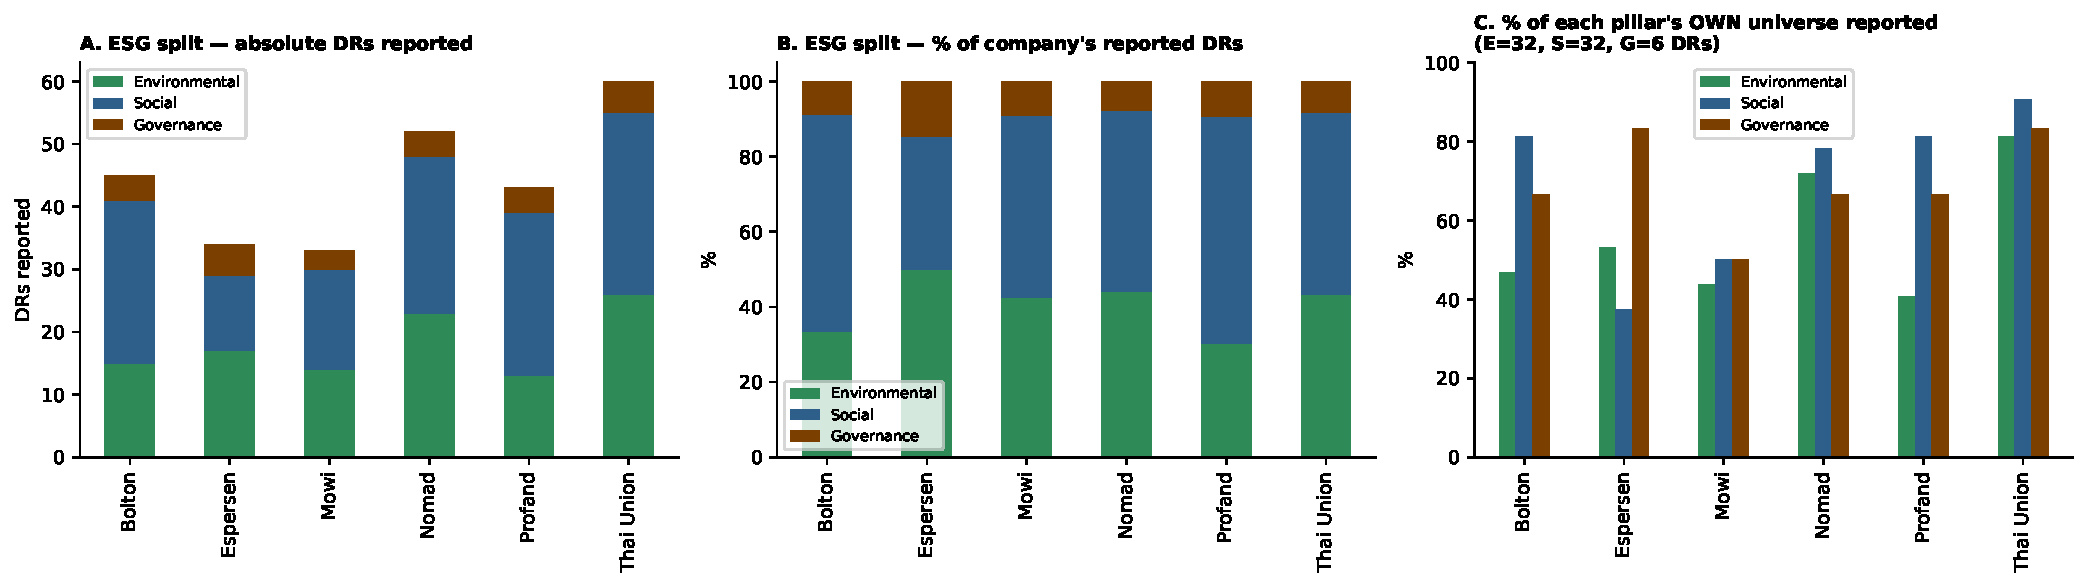
\includegraphics[width=\linewidth]{phase1/p1_esg_split.pdf}
\caption{ESG composition of each firm's reported DRs: in absolute terms
(panel~A), as a share of the firm's total reported DRs (panel~B), and as a
share of each pillar's own ESRS universe - 32 DRs each for Environmental
and Social, 6 for Governance (panel~C). By volume, Social is the largest
block and Governance the smallest for every firm (A--B); normalized by
pillar size, Governance is the most thoroughly covered pillar (C).}
\label{fig:p1-esg}
\end{figure}

\begin{figure}[htbp]
\centering
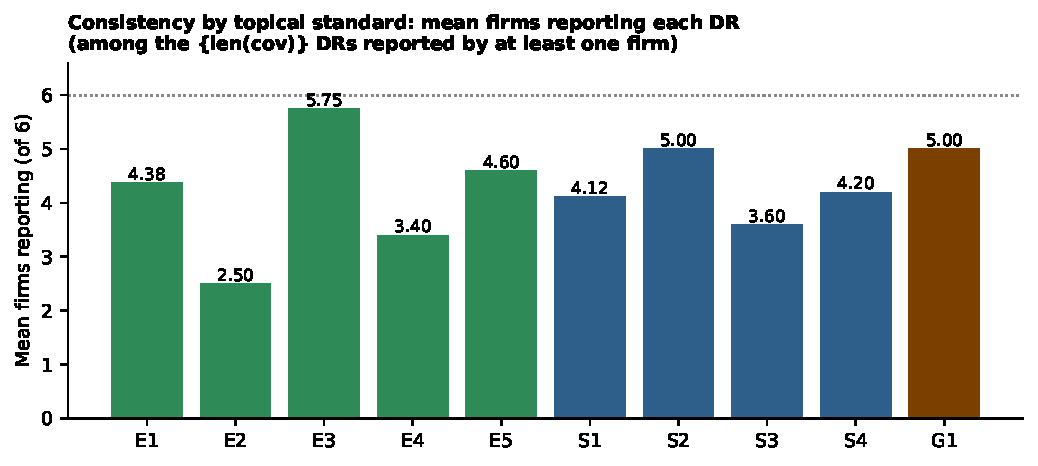
\includegraphics[width=0.75\linewidth]{phase1/p1_consistency.pdf}
\caption{Consistency by topical standard: mean number of cohort firms
reporting each DR, among the 63 DRs reported by at least one firm.
Consistency is highest for water (E3) and governance (G1); lowest for
pollution (E2) and affected communities (S3).}
\label{fig:p1-consistency}
\end{figure}

\FloatBarrier
\subsection{5.7 Robustness across sourcing models and reporting
year}\label{cohort-robustness}

\textbf{Does the core depend on sourcing model?} Because the cohort deliberately
spans four sourcing models, the universal core can be tested for whether it is an
artefact of one type of firm. It is not: the 13 core requirements are reported
across all four sourcing models - wild-capture, aquaculture, integrated
wild-plus-aquaculture, and diversified multi-species sourcing alike. All six
firms remain seafood \emph{processors} throughout; what varies between the four
groups is only what and how each sources - not whether processing is what
they do. Sourcing model changes only the \emph{edges} of the
picture, not the centre: model-specific topics such as feed and animal health
(aquaculture) or wild-stock status (wild-capture) appear only in the long tail,
while the climate, water, governance and workforce core is common to all. This
is confirmed rather than merely illustrated: because these 13 requirements are
by definition reported by \emph{all six} cohort firms, every sourcing-model
subgroup necessarily reports them too - there is no possible split by which
they could fail to be cross-model.

Two further checks confirm the core is not an artefact of the sample. First,
\emph{threshold sensitivity}: the near-universal set contracts smoothly with the
cut - 60 requirements are reported by at least two firms, 54 by at least three,
49 by at least four, 28 by at least five, and 13 by all six - so the $\geq$5-of-6 line sits on a gradient rather than a
cliff edge: the shortlist shrinks smoothly as the threshold tightens, with no
sharp jump at any single cut, so the choice of $\geq$5-of-6 is not an arbitrary
point that the result hinges on. Second, \emph{cohort-size invariance}: re-deriving the near-universal
set on the five European firms alone, dropping the non-European Thai Union at the
equivalent $\geq$4-of-5 cut, returns the \emph{identical} 28-requirement set - a
complete overlap, so the backbone does not depend on which firms are in the
cohort (Figure~\ref{fig:p1-cohort-invariance}).
Thai Union itself, the single non-EU firm and the broadest reporter (60 of
70), reports \emph{more} widely on biodiversity, affected communities and
pollution than the European average. This thesis does not investigate why
that pattern holds, and no assumption about its cause, whether GRI's broader
reporting scope, company-specific policy, or any other factor, is made here;
the observation is reported descriptively and left at that. What matters here is only that one requirement is reported
uniquely by Thai Union, so the consensus core survives the EU/non-EU divide
as common ground rather than an EU-regulatory artefact. In short, the same 13-topic core emerges whichever way the cohort is cut
- by the reporting threshold, by which firms are included, and by EU versus
non-EU - which is what lets it be read as a genuine feature of the sector rather
than a quirk of this particular sample.

\begin{figure}[htbp]
\centering
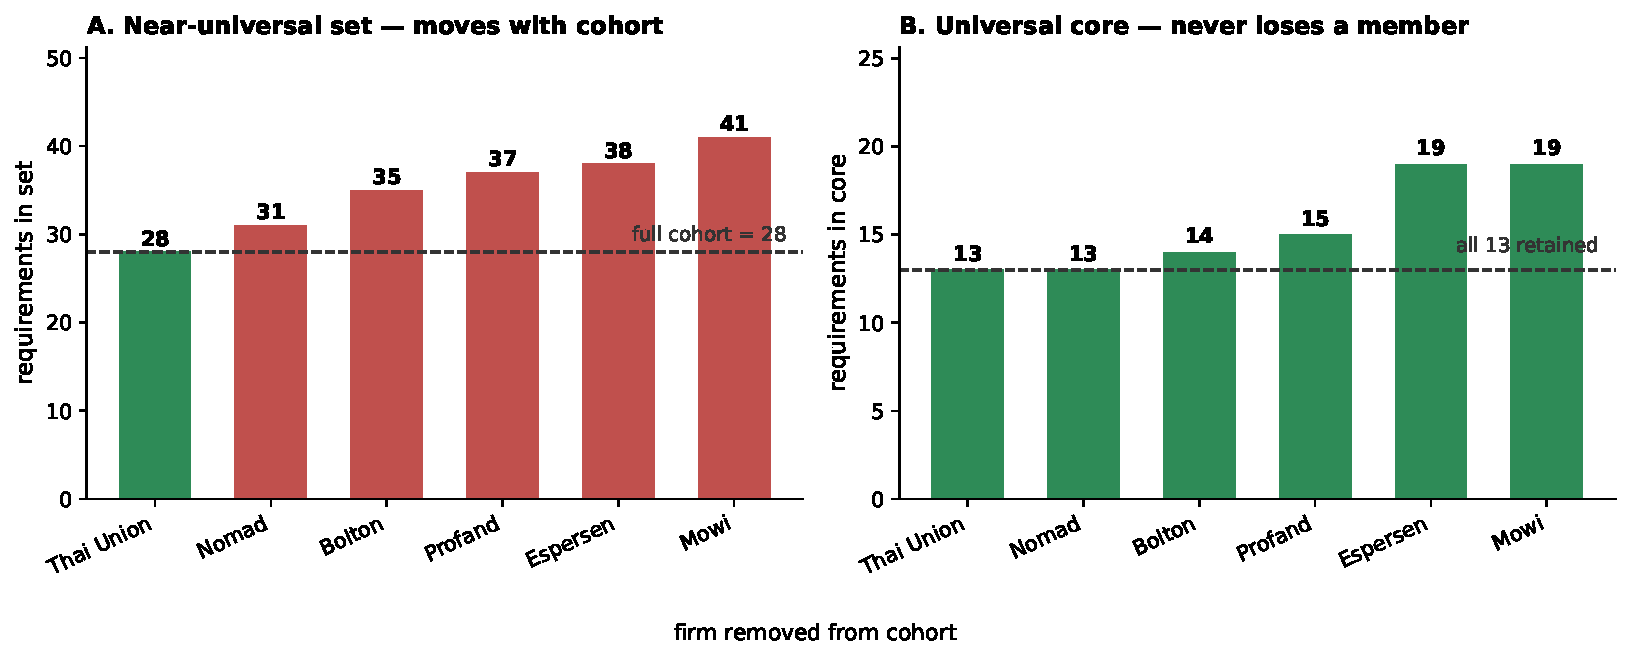
\includegraphics[width=0.7\linewidth]{phase1/p1_cohort_invariance.pdf}
\caption{Cohort-size invariance: the near-universal set (28 DRs) is
identical whether derived from the full six-firm cohort at the
$\geq$5-of-6 threshold or from the five European firms alone at the
equivalent $\geq$4-of-5 threshold.}
\label{fig:p1-cohort-invariance}
\end{figure}

Finally, an \emph{exploratory} observation, not a statistical result. The cohort
mixes 2024 and 2025 reporting years, and for the three firms with two comparable
years reported coverage was flat or fell very slightly - Nomad Foods from 53 to 52
DRs, Profand unchanged at 43, and Espersen from 36 to 34 - driven by a handful of
requirements dropped and none added (Figure~\ref{fig:p1-year}). With only
three firms over two years, no weight can be placed on this beyond its direction;
the main analysis uses each firm's most recent report (the figures in
Table~\ref{tab:cohort-r}). It runs against the
assumption of ever-expanding disclosure, and a comparable direction appears at
scale. The first large-scale longitudinal study of double-materiality outcomes
under the CSRD, covering 241 large listed EU companies, finds materiality rates
declining moderately between FY2024 and FY2025, concentrated in the
environmental standards other than climate (Nahrstedt, 2026). That study measures
which topics firms judge \emph{material}, not how much they disclose, so it is a
parallel indicator rather than a direct comparison; the two nonetheless move the
same way. The discussion returns to this under the Omnibus simplification.

\begin{figure}[htbp]
\centering
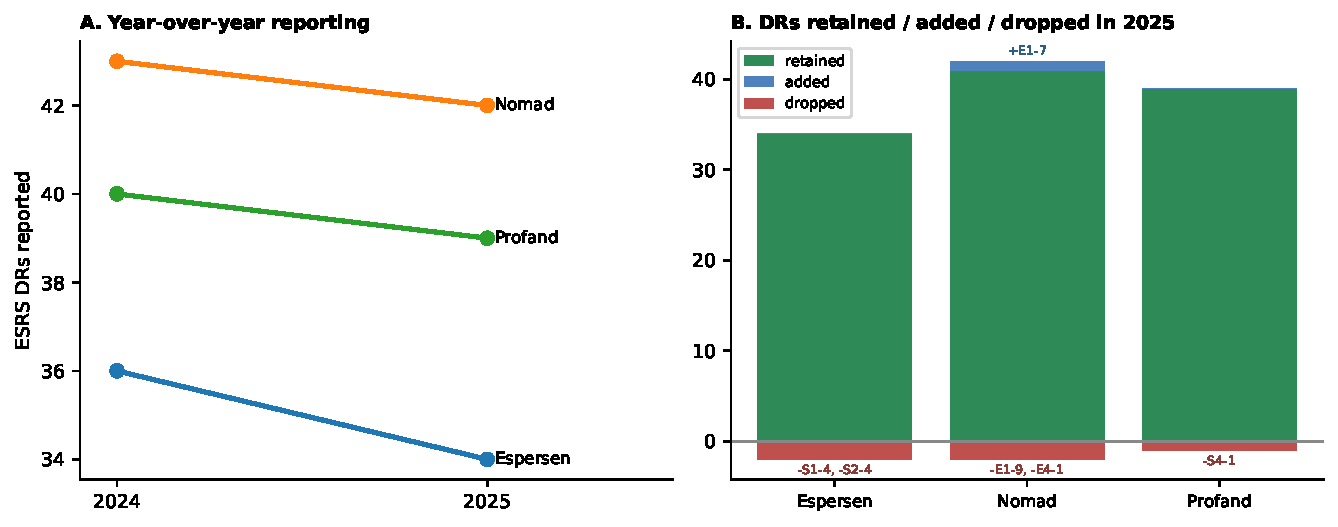
\includegraphics[width=\linewidth]{phase1/p1_year_evolution.pdf}
\caption{Year-over-year reporting for the three firms with both a 2024 and
a 2025 report. Panel~A: total DRs reported, which fell for all three.
Panel~B: requirements retained, added and dropped in 2025 - change is
dominated by retention, with a small net reduction.}
\label{fig:p1-year}
\end{figure}

\FloatBarrier
\subsection{5.8 What the cohort establishes - and what it does
not}\label{cohort-limits}

The cohort establishes three things. It fixes the height of the sector's
disclosure frontier at 53 requirements for the deepest reporter and around
57\% of the screened set for the median large firm; it identifies a
13-requirement universal core spanning climate, water, governance and
workforce that constitutes the sector's de facto baseline expectation; and it
locates the sector's collective gaps in the anticipated-financial-
effect and pollution requirements. Together these calibrate the realistic
disclosure ambition for a smaller firm and supply the empirical anchor for
the cross-framework demand mapping that follows.

\textbf{What this means for the SME question.} Read together, these findings do
more than describe the frontier; they bound the smaller firm's problem. Because
even the best-resourced reporters converge on a compact, cross-cutting backbone
rather than reporting everything, the SME's task is not to approximate an
ever-expanding frontier but to build a short, stable set of disclosures the sector
has already revealed to be expected - and that a firm is, on the
demand-relevance reading, most likely to be asked for. This is the hard
step described at the start of this chapter (Section~5.1); the
contribution here is to make it concrete for one sector by naming the
topics on which it should begin. That neither disclosure nor declared
materiality is expanding in the early CSRD years (Nahrstedt, 2026) only
strengthens the case for a proportionate, prioritised starting point
over open-ended completeness. \emph{Which} of these topics an individual firm
should build first, given the specific demands it faces, is the question the
cross-framework mapping takes up next.

Its limits are equally definite and are stated so that the findings are
not read beyond what they support. The cohort is a purposive sample of six
upper-bound reporters and is not representative of the sector, so no claim
about typical or average practice is made. Coverage is binary presence at
DR level and speaks to breadth, not to the depth, quality or assurance of
disclosure. The mapping from mixed ESRS and GRI source documents onto the
ESRS requirement set rests on analyst judgement, for which the member-checking
step described in Chapter~3 is a corroboration still outstanding rather than a
completed control. And the analysis is a 2024--2025 snapshot of a rapidly moving
reporting landscape. Within these
bounds, the cohort provides what it was designed to provide: a defensible,
document-grounded map of the seafood disclosure frontier.


% =====================================================================

\FloatBarrier
% =====================================================================
% STEPS 3-4 - CROSS-FRAMEWORK DEMAND MAPPING: WHERE TO BUILD FIRST
% Self-contained modular chapter, drafted from the authoritative main.tex
% methodology (§4.5 Phase 3, §4.6 Phase 4, §4.7 Phase 5, §4.8 validation)
% and the Results section (composition + first action points).
% Numbers reconciled to the current dataset (v8 Excel / tool):
%   rows = 33 topics; cols = 31 (30 scored instruments, VSME split);
%   1023 cells, 188 filled (18%);
%   source 12/11/3/5; tiers 12/7/8/4 (VSME=Customer).
% Figures: fig:cell-coding (TikZ, needs tikz+libs in preamble - already in main),
%   topic_distribution.pdf, r_actor_tier.pdf, r_stage_system.pdf.
% =====================================================================

\section{6. Cross-framework demand mapping: where to build
first}\label{angle3-crossmapping}

This chapter covers two steps rather than one. Step~1 (Chapter~4) fixed the
\emph{columns}: the instruments that make up the disclosure ecosystem and how
binding each is. Step~2 (Chapter~5) fixed the \emph{rows}: the disclosure topics
the sector's leading firms actually report, narrowed to a cohort-evidenced
universe.

Step~3, the \emph{overlap}, crosses the two. It scores \emph{who demands what},
topic by topic and instrument by instrument, then reads the resulting matrix for
the thesis's central question: given a fragmented wall of overlapping demands,
which topics satisfy the most of them if built first. Step~4, \emph{building the
tool}, turns that finding into a decision a firm can act on - a short ranked list
of topics to build first, and a diagnostic that tailors the list to its own
situation. Together the two steps answer the third research question and produce
the thesis's central practical contribution.

Figure~\ref{fig:coverage-matrix-screenshot} shows a representative excerpt of the
underlying coverage matrix, so the scale and shape of the raw scoring are visible
before the chapter turns to how it is built.

\begin{figure}[htbp]
\centering
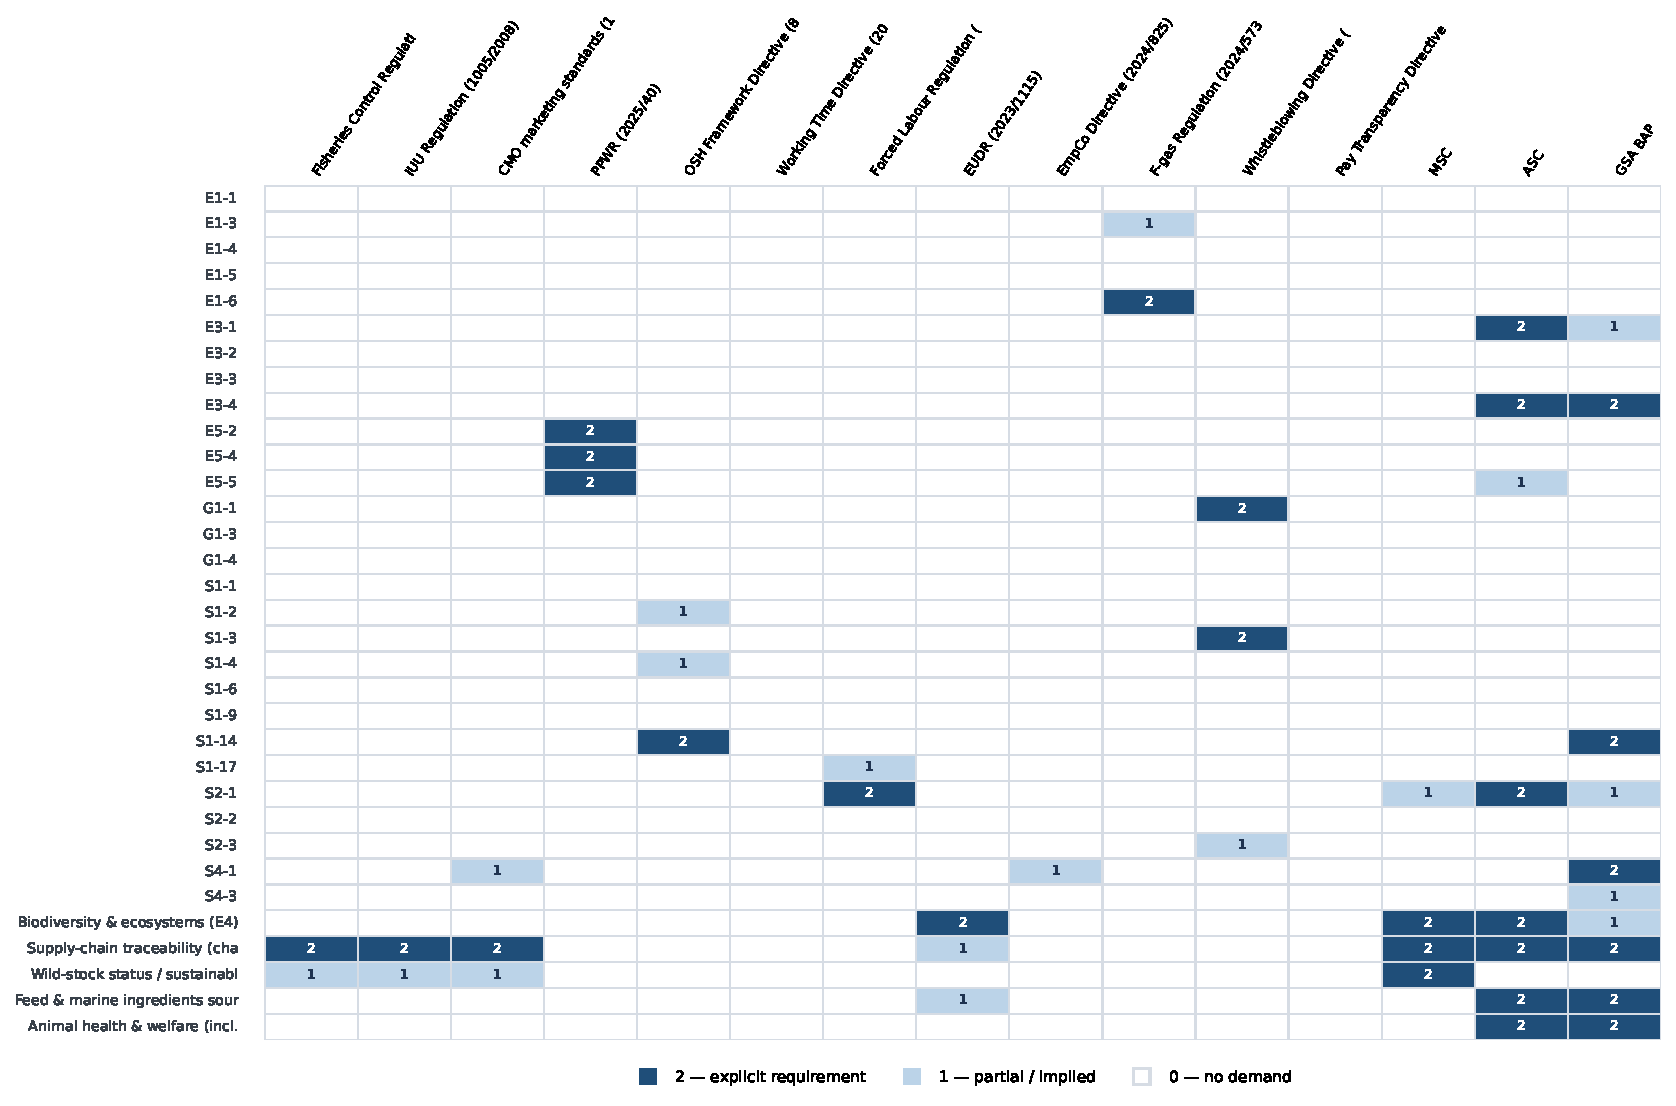
\includegraphics[width=\linewidth]{phase3/appendix_figures/coverage_matrix_screenshot.pdf}
\caption[Representative excerpt of the coverage matrix]{Representative excerpt
of the coverage matrix (\emph{Phase3\_\allowbreak Coverage\_\allowbreak
Matrix\_\allowbreak v18.xlsx}, sheet ``Coverage matrix''): topic rows
against scored-instrument columns, coloured by score (0/1/2). Shows all 33 topic
rows and the first 15 of the 31 scored instrument columns (Tier~1--2); the full
matrix is in the source workbook.}
\label{fig:coverage-matrix-screenshot}
\end{figure}

\FloatBarrier
\subsection{6.1 The convergence logic}\label{cm-theory}

The move from a wall of demands to a short build-first list rests on one idea:
that the demands, though issued by different actors in different vocabularies,
draw on a much smaller set of underlying capabilities, so that a single
capability can answer many demands at once. Two established literatures make this
precise. The first is the \emph{resource-based view} of the firm and the
dynamic-capabilities tradition (Barney, 1991; Teece, 2007), which treat the
ability to produce and reuse structured data as an organisational capability that,
once built, is redeployable across uses at low marginal cost. The second is
\emph{stakeholder-salience} theory (Mitchell, Agle \& Wood, 1997): a firm facing
many legitimate claimants cannot serve each separately and must triage, and the
rational triage is toward the topics on which the most salient claimants converge.
Salience in that account is the combination of three attributes - the
\emph{power} to impose consequences, the \emph{legitimacy} of the claim, and its
\emph{urgency} - and the tiering of Chapter~4 is essentially an empirical reading
of the first two: a Tier~1 legal obligation carries power and legitimacy
together, a Tier~4 voluntary commitment neither. To these three the SME case adds
a fourth constraint that Mitchell's framework treats as given, namely the
\emph{resources} available to answer any claim at all. Triage for a
resource-constrained firm is therefore not only a question of which claimants
matter most, but of how few distinct capabilities the answer can be built from -
which is what the convergence measure below is designed to capture.

Convergence is therefore the organising construct. Where a topic is demanded by a
regulator, an investor framework and an industry standard alike, capability built for that topic is not spent once but several
times over - the compound return that distinguishes a proactive posture from a
reactive one (Chapter~2). A topic demanded through only one channel yields a
narrower return. The analytical task of this chapter is thus to \emph{measure}
convergence across the fragmented landscape and to identify the topics where it is
highest - the hotspots at which building once satisfies many.

\FloatBarrier
\subsection{6.2 Assembling the matrix: rows and
columns}\label{cm-matrix-build}

The matrix has rows and columns, and neither comes straight from the previous
chapters. The rows start from the topics the cohort actually reports
(Chapter~5), which are then trimmed to those the sector agrees on and extended
with four topics the ESRS has no row for. The columns start from the instruments
catalogued in Chapter~4, which are then cut back to those that genuinely ask the
processor for something. Both changes are set out here, before any cell is
scored, because what goes into the matrix decides what it can show: a row for a
topic nobody is asked about, or a column for an instrument that demands nothing,
would distort every count taken from it.

\textbf{Rows: from the cohort frontier to the topic universe.} The rows begin from
the cohort frontier (Chapter~5) and are built up in three steps:

\begin{enumerate}
\item \textbf{The requirements the cohort converges on enter directly} - those
reported by at least five of the six firms. These are the topics the sector's own
practice has revealed to be expected (28 requirement-level rows). The set includes
the climate transition plan (E1-1), which reaches the cut only after the direct
screening of report bodies described in Section~\ref{cohort-method}, because no
GRI disclosure maps to it.

\item \textbf{One topic clears the same bar one level up.} Biodiversity (E4) is
reported by at least five firms when a firm counts as covering the topic if it
reports \emph{any} of the topic's requirements, but no individual E4 requirement
reaches the five-of-six cut on its own - the best-reported reach four. E4
therefore enters as a topic-level row: the same consensus rule at coarser
granularity, not an expert-judgement exception. Consumers and end-users (S4) was
admitted the same way in an earlier version of this analysis; after the bridge
rebuild two of its requirements, S4-1 and S4-3, clear the cut individually, so S4
is now represented at requirement level and needs no topic-level rescue. With the
requirement-level set it forms the cohort-evidenced core (29 rows).

\item \textbf{Four seafood-defining topics have no ESRS home at all} and are
carried in against the GRI~13 sector standard and EU sector legislation:
supply-chain traceability, wild-stock status, feed and marine ingredients, and
animal health and welfare (antimicrobial use folded into the last). These are
flagged as sector-material rather than cohort-evidenced. Each carries a
production-system tag - wild, aqua or both - so a firm drops the rows that do not
concern it.
\end{enumerate}

The funnel therefore runs from the 70 topical ESRS disclosure requirements, narrows
to the cohort-evidenced core, then \emph{extends} by four. Those four are the one
place where the ESRS blueprint is insufficient and the sector standard supplies the
rows instead. Stated as a sequence, with each figure used once:

\begin{enumerate}\itemsep2pt
\item \textbf{70} topical ESRS disclosure requirements form the starting universe
(Chapter~5).
\item \textbf{28} of those are reported by at least five of the six firms at
requirement level, and enter directly. E1-1 is among them, reached through the
body screening of Section~\ref{cohort-method} rather than through the bridge.
\item \textbf{+1} topic-level row, biodiversity (E4), where the topic clears the
consensus cut but no single requirement within it does - giving \textbf{29}
cohort-evidenced rows.
\item \textbf{+4} sector-material rows carried in from GRI~13 and EU sector law,
for which no ESRS requirement exists: supply-chain traceability, wild-stock
status, feed and marine ingredients, and animal health and welfare.
\item \textbf{33} rows in total, scored against \textbf{31} instrument columns -
30 instruments, with the VSME split into its Basic and Comprehensive modules -
giving the \textbf{1{,}023} cells of the matrix.
\end{enumerate}

They are not chosen ad hoc. Each of GRI~13's 26 material topics
(Agriculture, Aquaculture and Fishing) was classified against the ESRS as
\emph{covered}, a \emph{reporting gap} (an ESRS mapping exists, but cohort
reporting on it falls below the $\geq$5/6 consensus threshold), or a
\emph{structural gap} (no ESRS disclosure requirement exists at all).

The four divide evenly between two of those categories. Animal health and welfare
and supply-chain traceability are structural gaps: the ESRS has no requirement
covering either, so nothing in the standard asks for them at all. Wild-stock
status and feed and marine-ingredient sourcing are different. Both are
production-specific disclosures nested inside biodiversity (GRI~13.3), which is
itself covered and already in the universe. The broad subject is therefore
present, but these two specific disclosures within it are not. The full
classification is given in \nameref{app:gri13}.

\textbf{Columns: from the full ecosystem to the scored instruments.} The columns
begin from the instruments catalogued in the ecosystem (Chapter~4). That
catalogue is deliberately the whole field, so it includes instruments that place
no scorable demand on the processor in the end. The scored set is the subset that
does.

Three groups are set aside. The \emph{context} instruments bind Member States
rather than the firm. The \emph{excluded} instruments fail the second of the two
admission gates screened at catalogue stage - ESG relevance first, then
organisation-level obligation - which are defined and applied instrument by
instrument in \nameref{app:scope}. The CSRD/ESRS standard is held out separately
as the \emph{baseline} reference against which the rows are defined, rather than
scored as one more demand.

That leaves \textbf{30} scored instruments. Only one of them, the VSME, is split
into two columns, for its Basic and Comprehensive modules, because it is the only
instrument with two officially defined and nested reporting tiers - which is why
30 instruments occupy 31 columns. Each scored column inherits its stakeholder
source and its obligation locus (direct, indirect or context) from Step~1. Some columns are switched off for a given firm because its profile puts
the instrument out of scope, and two kinds of switch apply. The first is the
production system: a wild-only firm switches off the aquaculture certifications
(ASC, BAP). The F-gas switch is separate from production system and turns on
equipment rather than sourcing: it is switched \emph{on} for the modelled firm,
since refrigeration is near-universal in seafood processing, and exists only for
the minority of sites that have already converted entirely to natural
refrigerants such as ammonia or CO\textsubscript{2} and hold no fluorinated gas.
The second switch is size: within the SME band several obligations turn on
headcount - the Pay Transparency Directive's gender pay-gap reporting applies from
150 employees and the whistleblowing obligation from 50 - so a firm below a
threshold switches off the instruments above it. A switched-off instrument is
excluded from that firm's demand sums, though a customer may of course still ask
for the same content contractually, in which case the demand reaches the firm
through the customer channel rather than the legal one. The full
instrument-by-instrument classification - scored, baseline, context or excluded,
with the reason for each - is provided in \nameref{app:scope}.

The demand matrix is therefore a grid of topic rows against instrument columns,
every cell recording how strongly a given instrument demands a given topic, on the
scale set out next.

\FloatBarrier
\subsection{6.3 Scoring the matrix}\label{cm-matrix}

\textbf{The coverage scale.} Each cell is coded on a three-level scale defined ex
ante:
\begin{itemize}
\item \textbf{0 - not covered:} the instrument does not address the topic, or its
demand maps only to datapoints outside the row universe (the out-of-frame rule
below).
\item \textbf{1 - touched:} the instrument references the topic but imposes no
binding requirement on any of its datapoints.
\item \textbf{2 - required:} the instrument explicitly and bindingly requires
the entity to achieve, address, comply with, certify, report on or disclose at
least one datapoint belonging to the topic.
\end{itemize}
Binding \emph{conformity} counts equally with binding \emph{disclosure}: a
mandatory recycled-content target (e.g.\ the PPWR), an accident-prevention duty
(e.g.\ the OSH Framework Directive) or a market-access prohibition on
forced-labour products (e.g.\ the Forced Labour Regulation) scores~2 even where
no report is filed, because it bindingly addresses the datapoint substance. The score
measures \emph{how strongly} an instrument demands a topic; it says nothing about
\emph{how} that demand reaches the firm, which is a different question. A demand that
arrives indirectly - CSDDD, which for the sub-threshold processor modelled here
binds its large customers and reaches it as a cascaded supplier requirement,
though it would bind a larger processor directly - is still scored on its
strength: if
it bindingly imposes a topic's datapoints it scores~2, exactly as a directly binding
rule would. Whether the route is direct or indirect is recorded separately, as the
obligation locus, and never raises or lowers the score. Keeping the two apart stops
an indirect-but-binding demand from being under-counted merely because it is
transmitted rather than imposed.

\textbf{Datapoint-grounded coding.} A score is assigned against the
\emph{constituent datapoints} of a requirement, not against the title of its
disclosure requirement. Each of the 29 cohort-evidenced rows is decomposed into
its official EFRAG datapoints using the ESRS datapoint master (Commission
Delegated Regulation (EU) 2023/2772): the 26 DR-level rows resolve to 356
datapoints and the two topic-level rows (E4, S4) to a further 152. An instrument
scores~2 where its indicators demand at least one of a requirement's datapoints,
1 where it references the topic but demands none of them, and~0 where it is
silent. This replaces the broad question of whether instrument~$f$ addresses
topic~$r$ with the concrete and reproducible one of whether~$f$ demands at least
one datapoint of~$r$. It also surfaces corrections. Whistleblowing demand, for
instance, resolves to the governance row that actually carries the whistleblowing
datapoints rather than to an adjacent anti-corruption row. Once such corrections
are logged they are findings about the coding process rather than matters of
method.

\textbf{When self-reporting counts as a binding demand.} Many instruments are
self-reported, which raises a scoring question with real consequences: whether
completing a supplier questionnaire places the same demand on a topic as reporting
against a defined standard. Treating the two alike would inflate the matrix, so a
single rule separates them - and what matters is not \emph{who} reports but whether
the \emph{datapoints are fixed in advance}:
\begin{itemize}
\item An \emph{open-question self-assessment}, where the firm describes itself
against broad prompts with no defined datapoints and no external threshold
(e.g.\ EcoVadis, the Sedex SAQ), shows the topic is relevant to the firm but
pins down no specific data. It scores~\textbf{1}.
\item A \emph{defined-datapoint standard}, where the datapoints to report are fixed
ahead of time - voluntary (GRI, CDP, TNFD) or mandatory (the ESRS) - imposes the
datapoint even though it too is self-reported. It scores~\textbf{2}.
\item An \emph{enforced-conformity} requirement, where the firm must meet a bar and
fix failures (a SMETA audit it must pass to keep the buyer, or a binding legal duty),
likewise scores~\textbf{2}.
\end{itemize}
A last line separates a rating the firm \emph{feeds} from one built \emph{about} it:
a rating is scored only where the firm must supply the data itself (EcoVadis,
scored~1); purely external ratings assembled from public data (MSCI, Sustainalytics,
the Dow~Jones Best-in-Class Indices) place no demand on the firm and are not scored
at all, since such a rating consumes disclosures rather than asking for them.

\textbf{Sector-material rows.} For the four seafood-specific gap rows
(traceability, wild-stock status, feed and marine ingredients, animal health and
welfare) no ESRS datapoint exists by construction; these are scored against the
criteria of the demanding instruments themselves - MSC Principle~1 stock-status
reference points for wild-stock, the GDST key data elements for traceability, and
ASC antibiotic and survival criteria for animal health and welfare. A pinned rule
prevents double-counting on the wild-stock/E4 boundary: stock-status and
legal-sourcing demand (MSC Principle~1, the IUU catch-certificate regime) codes
to the wild-stock row, whereas generic biodiversity and
ecosystem-impact demand (ESRS~E4, GRI~101, TNFD, MSC Principle~2 on bycatch and
habitat) codes to E4; a single instrument may legitimately score on both rows
through different provisions.

These four rows are not equivalent kinds of measure, and the distinction matters
for how their scores should be read. Wild-stock status is an \emph{outcome}: it
asks whether the stock a firm buys from is healthy, and answering it requires
stock assessment science and reference points the processor does not generate
itself. Supply-chain traceability is an \emph{assurance mechanism}: it
establishes that a product came from where it is claimed to have come from, and
says nothing on its own about whether that source is sustainable. A firm can
operate complete traceability on a stock that is severely overfished. The high
demand score traceability carries in this matrix therefore records how many
instruments require it, not that meeting it evidences a sustainability outcome.
The two rows are kept separate for exactly this reason, and the build-first
ranking that follows should be read as a map of what the environment
\emph{asks for} rather than of what most improves the state of the resource.

\textbf{Are wild-stock status and traceability actually live practice, not
just a GRI category?} Neither has an ESRS DR, so neither was captured by the
cohort's DR-level coverage coding in Chapter~5 - which raises a fair
question: is including them here just following GRI~13's classification, or
is there evidence the sector's own leading firms actually treat them as
real, active topics? All six cohort firms do, on both counts
(Table~\ref{tab:sector-material-evidence}).

\begin{table}[H]
\centering
\caption{Sector-material topics in the cohort's own reporting. Each firm
discloses both a sustainable wild-sourcing certification level and a
traceability system, though neither topic has an ESRS disclosure requirement.
Figures as published by each firm; wording follows the source report.}
\label{tab:sector-material-evidence}
\footnotesize
\begin{tabularx}{\textwidth}{@{} l X p{4.5cm} @{}}
\toprule
\textbf{Firm} & \textbf{Sustainable sourcing, as reported} & \textbf{Traceability} \\
\midrule
Thai Union (2024) & 98.9\% of tuna MSC-certified, in MSC assessment, or FIP-covered & Working toward GDST compliance \\
Bolton (2024) & 99.7\% of tuna from responsible fishing practices: MSC-certified, in full MSC assessment, or covered by a credible and comprehensive FIP & Working toward GDST compliance \\
Nomad Foods (2025) & 99.9\% of fish and seafood certified sustainable or responsibly sourced & Own digital traceability system \\
Espersen (2025) & 99\% of fish and seafood sourced in accordance with third-party certification & Own electronic traceability system \\
Mowi (2025) & 100\% of harvest volume certified to a GSSI-recognised standard (ASC, BAP or GLOBALG.A.P.) & Own digital traceability system \\
Profand (2025) & MSC- and ASC-certified sourcing & Active GDST participant \\
\bottomrule
\end{tabularx}
\end{table}
The figures in the middle column are not comparable across firms and are not
used comparatively here. Each firm defines its own numerator: some report
certified volume alone, others bundle certified volume with product in
assessment and with fisheries covered by improvement projects, and some state a
figure for one species rather than the whole portfolio. The column records that
each firm makes a sourcing claim and on what basis, not how the firms rank
against one another; no claim in this thesis rests on the difference between
99.9\% and 98.9\%.

The two topics fall outside the ESRS structure this thesis uses as its main
coordinate system, but they are not a marginal or invented addition: every
firm in the cohort reports on both, independently of each other and of GRI~13's
classification. This is stated here as corroboration, not as scored
evidence - these mentions were not coded against a defined datapoint set
the way the 70-DR cohort analysis was, so no coverage percentage is claimed
for them.

\textbf{Does this reach a firm that only processes, not farms or fishes?} A
pure processor buys already-caught or already-farmed product; it does not
manage a stock or run a farm. So how much of the wild-stock, feed and
animal-welfare demand above actually lands on it? All of it, but in two
different ways, and the matrix tags which is which. \emph{Direct}: the
processor itself holds a Chain-of-Custody (CoC) certificate (MSC, ASC,
GLOBALG.A.P., BAP, Friend of the Sea) and keeps its own segregation and lot
records to prove it - this is an obligation on the processor itself.
\emph{Indirect}: to hold that CoC certificate at all, its supply contracts
must specify sourcing from a stock, farm or feed mill that meets the
scheme's upstream standard - for instance MSC Principle~1 on stock health, or
ASC's feed and antibiotic limits. These are illustrative rather than exhaustive:
both schemes are full standards, and a supplier is certified against the whole
of one, not against a single principle. MSC covers stock status, environmental
impact and management system across its three principles, and ASC likewise
extends well beyond feed; no buyer accepts conformity with one principle alone.
The examples are named here only because they are the clauses through which the
upstream demand reaches the \emph{processor}.

This transmission also runs in the other direction, which qualifies the common
assumption that a processor is simply a demand-taker. A purchasing policy that
specifies certified sourcing exerts real pressure upstream, and a large enough
book of such policies can move a fishery: the Argentine hake fishery
(\emph{Merluccius hubbsi}) has moved toward MSC assessment in response to buyers
declining uncertified product (O.~Spring, Group Sustainability Manager, Nomad
Foods, personal communication, August 2026). The effect is weaker for a single sub-threshold SME than for a
large buyer, but it is not absent, and it is one route by which a small
processor's disclosure capability converts into influence rather than only cost.

The processor doesn't manage the upstream operation, but
it cannot keep its certificate without sourcing from one that does - so
the demand is real, just transmitted rather than performed directly. Each
cell is scored on the same 0/1/2 strength scale either way (a core
criterion such as MSC~P1 stock status or ASC feed-conversion limits scores~2,
a lighter good-practice mention~1); direct or indirect only records \emph{how}
the demand reaches the processor, and - as stated above - never changes the score itself.

One locus tag needs qualifying. EUDR's due-diligence duty on feed and
marine-ingredients sourcing binds the feed manufacturer importing raw soy or
palm, not a processor further downstream buying finished feed. For the modelled
sub-threshold processor the demand therefore arrives indirectly, through the feed
supplier's own compliance. The source workbook records obligation locus once per
instrument column rather than per cell, so EUDR carries a single \emph{direct}
tag there; the qualification stated here applies to the feed row specifically.
Because locus is descriptive and never enters the score, no coverage figure in
this chapter is affected.

\textbf{Out-of-frame demand.} Some indicator-level demand maps cleanly onto an
ESRS datapoint that lies \emph{outside} the cohort-defined universe: the Pay
Transparency Directive's gender pay-gap requirement maps to S1-16, the Working
Time Directive to S1-11/S1-15, none of which cleared the $\geq$5/6 consensus and
so have no row. Such demand scores~0 against the in-universe rows and is
\emph{not} reassigned to the nearest available row (which would misattribute and
inflate it); instead it is recorded in a separate out-of-frame register
(instrument~$\rightarrow$ demanded DR~$\rightarrow$ reason). A framework's
contribution to the matrix is thus the \emph{intersection} of its demand with the
cohort-evidenced universe, not the union of everything it asks.

This produces a finding in its own right rather than a mere bookkeeping note.
\textbf{Mandatory labour-standards disclosure and the voluntary reporting
universe occupy partly disjoint spaces.} EU labour law requires disclosures -
adequate wages, work-life balance, working-time protections - that the sector's
own leading reporters largely do not make, because those requirements never
clear the consensus threshold that defines the topic universe. The demand is
legally binding and the reporting practice has not followed it. For a firm, this
means the build-first set derived here does not discharge its labour-law
obligations, which have to be met whether or not peers report against them; for
policy, it marks a place where mandatory demand and voluntary convergence have
not met, and where the assumption that market practice will carry legal
requirements does not hold.

\textbf{Methodology providers versus disclosure askers.} Instruments that supply
methods but do not themselves pressure an entity to report - e.g.\ the GHG
Protocol or the ISO standards such as ISO~14001 - are held in an enabling layer
and excluded from the demand sums, distinct from the disclosure askers (e.g.\
CDP, SBTi, MSC) that require an entity to submit or certify information. The
same treatment applies to the food-safety schemes: BRCGS and IFS require chain
of custody and full traceability, and so materially help a processor meet the
traceability row, but they are certification programmes a buyer requires rather
than disclosure demands in their own right, and are therefore carried as
enablers rather than scored columns. Scored cells are documented in a
justification log giving a one-line rationale, a citation to the source clause or
indicator, and the identifier(s) of the ESRS datapoint(s) the demand maps to -
the audit trail that protects the coding against challenge. The log covers 120 of
the 188 scored cells. The 68 without an individual entry are concentrated in a
small number of instruments whose scoring logic is uniform across topics - the
Sedex self-assessment questionnaire accounts for 15 of them, GSA BAP for 8 - where
the rationale is given once at instrument level in the coding protocol rather than
repeated per cell. The gap is therefore one of documentation granularity rather
than of unrecorded judgement, but it is stated here so the audit trail is not
claimed to be more complete than it is. The complete coded
matrix and its justification log, together with the per-cell coding protocol,
are provided in \nameref{app:matrix} (Figure~\ref{fig:cell-coding-appendix}). A
representative excerpt of the scored matrix itself is shown in
Figure~\ref{fig:coverage-matrix-screenshot} at the start of this chapter.

\FloatBarrier
\subsection{6.4 Hotspot measures and stage
assignment}\label{cm-staging}

With the matrix populated, the columns are collapsed into the four
stakeholder-driver channels (regulator, customer, investor, industry/NGO), and two
complementary measures are computed for every topic:
\begin{itemize}
\item \textbf{Breadth ($\Sigma$)} - how much demand a topic attracts in total: add
up its scores across every instrument, counting a binding requirement (2) as double a
passing mention (1). A high breadth means many instruments ask for the topic, or a
few ask for it bindingly. It measures the \emph{volume} of demand.
\item \textbf{Convergence (0--4)} - the number of the four stakeholder channels
in which at least one instrument demands the topic. Because it counts
\emph{channels}, not instruments, it is robust by construction to within-channel
repetition (five overlapping certifications collapse to a single customer signal)
and captures cross-stakeholder consensus rather than sheer volume.
\end{itemize}
Convergence is the primary signal and breadth the secondary one: convergence is
the dedup-robust measure of how widely the fragmented landscape agrees on a topic,
while breadth - which overlapping instruments can inflate - discriminates
between topics of equal convergence.

Topics are then triaged into three stages on the two measures jointly:
\begin{itemize}
\item \textbf{Stage~1 - build first:} convergence $\geq 3$ \emph{and} breadth
$\geq 12$. Demanded across at least three of the four channels \emph{and} in the
top quartile of demand volume - the no-regret core, where capability built for
one channel serves several.
\item \textbf{Stage~2 - next:} convergence $\geq 3$ but breadth below the
quartile cut. Broad consensus, less intense demand; build after the core.
\item \textbf{Stage~3 - monitor:} convergence $\leq 2$. Demanded through only one
or two channels; required for compliance where in scope, but not yet drawing broad
demand.
\end{itemize}
Both thresholds are anchored in the empirical distribution rather than set
arbitrarily (Figure~\ref{fig:topic-distribution}). The convergence cut of three is
the simple majority of the four channels. The breadth cut of twelve is the
\emph{third quartile} of the breadth distribution across the 33 topics, so the
Stage-1 volume gate selects the top quartile and recalibrates automatically if the
scores change. In the modelled firm no topic below convergence three reaches the
breadth cut, so the two criteria identify one coherent Stage-1 set rather than two
competing ones.

\begin{figure}[htbp]
\centering

\includegraphics[width=\linewidth]{topic_distribution.pdf}
\caption{Distribution of cross-framework demand across the 33 topics for the
modelled firm. (A)~Breadth $\Sigma$ (volume of demand); the Stage-1 cut is the
third quartile, Q3~$=12$. (B)~Convergence - the number of the four stakeholder
channels demanding each topic. (C)~The two-axis staging map: Stage~1 (\emph{build
first}) requires both broad consensus (convergence $\geq 3$) and high volume
(breadth $\geq 12$); the shaded region is the Stage-1 set. All 33 topics are
plotted in panel~C, but only the nine Stage-1 topics and the nearest few below
the cut are labelled, to keep the panel legible; the remaining points are
unlabelled rather than absent. E1-1, the climate transition plan added to the
universe by the bridge rebuild, plots at breadth~8 and convergence~3 and so
falls below the volume gate.}
\label{fig:topic-distribution}
\end{figure}

\FloatBarrier
\subsection{6.5 The composition of the demand
environment}\label{cm-composition}

The populated matrix is read first as a description of the demand
\emph{environment} the modelled sub-threshold SME (50--250 employees, non-tuna)
faces. Its 31 scored columns are distributed unevenly across the four channels
(Figure~\ref{fig:r-actor-tier}): the environment is dominated by regulators (12
columns) and customers (11), which together account for 23 of the 31 columns
(74\%), while investors are the thinnest channel (3) and industry/NGO initiatives
the remainder (5). The necessity tiers fall 12/7/8/4 across Tiers~1--4, so the
regulatory legal-licence layer is the single largest block.

The matrix is sparse by construction: of the 1{,}023 instrument$\times$topic cells,
188 (18\%) carry a demand, split almost evenly between \emph{binding} requirements
(92 cells scoring~2) and \emph{touched} references (89 cells scoring~1). The demand
environment is therefore not a dense web in which every framework touches every
topic, but a structured field in which a minority of concentrated, mostly
regulator- and customer-borne demands define the landscape.

Source and necessity
tier are coded on independent criteria, yet the two axes correlate: the
instruments at Tier~4 (strategic differentiation) cluster almost entirely in the
industry/NGO channel (SBTi, the UN Global Compact, voluntary coalitions), while
the binding licence-to-operate tiers are dominated by the regulator channel.
Strategic, proactively-adopted initiatives tend to be NGO- or coalition-run rather
than regulator-mandated or capital-demanded. This is more than the truism that
voluntary means non-mandatory: it locates \emph{who owns the elective frontier}. For a
seafood processor, the route to a proactive posture therefore runs through
civil-society standards rather than through the state or the capital markets. The
sector's voluntary leadership agenda is set by NGOs and coalitions, not by
investors - a point the discussion returns to.

\begin{figure}[htbp]
\centering
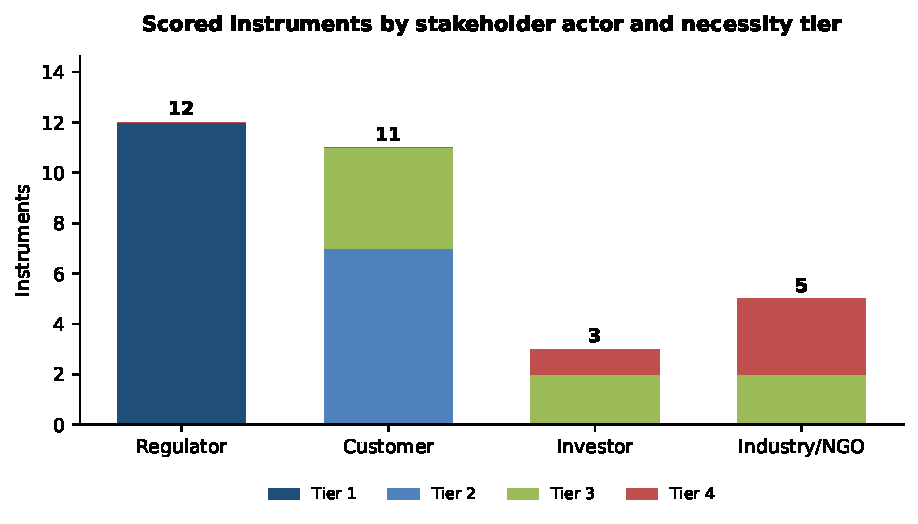
\includegraphics[width=0.78\linewidth]{r_actor_tier.pdf}
\caption{Composition of the scored demand environment: the 31 instrument columns
by stakeholder channel and necessity tier. Regulators and customers dominate;
investors are the thinnest channel.}
\label{fig:r-actor-tier}
\end{figure}

\FloatBarrier
\subsection{6.6 Narrow law, broad cascade}\label{cm-narrow-broad}

A second pattern concerns not \emph{who} demands but how \emph{broadly} each
instrument demands, and it reframes the SME's problem. Individual regulations are
narrow: each of the twelve regulatory instruments touches on average only two
topics, and none more than three - the Packaging and Packaging Waste Regulation
covers waste and packaging, the occupational-health directive covers health and
safety, the F-gas Regulation covers emissions. Breadth - and therefore the
overlap that creates the SME's burden - comes overwhelmingly from the market and
voluntary side: customer instruments demand on average nine topics each (the CSDDD
eighteen), and industry and NGO reporting frameworks almost eight (GRI alone
twenty-five).

The wall of overlapping demand is therefore not the product of the SME being
directly over-regulated. It is the product of a few \emph{broad} horizontal
instruments - CSRD, CSDDD, SFDR - that apply to the firm's large customers and
financiers and \emph{cascade} down the value chain as supplier questionnaires,
together with the voluntary certification and rating landscape. Direct regulation
on the processor is targeted and lean; the breadth is transmitted, not imposed.
This has a direct consequence for what an SME should do. The broad horizontal
instruments that generate the cascade - CSRD and its ESRS - are also, ultimately,
the most \emph{comprehensive} statement of what will be asked: a firm fully aligned
to the ESRS would, for the general-sustainability topics, already hold almost
everything a customer or financier could cascade down to it. Full ESRS alignment is
therefore the sensible end-state. But it is a large ask for a resource-constrained firm,
and in the interim the demand actually placed on SMEs is being deliberately capped - by the VSME and by the Omnibus value-chain provisions - to a proportionate
subset. The pragmatic path this chapter identifies sits between the two: rather than
attempt full alignment at once or simply wait for the caps to settle, a firm builds
first the \emph{most convergent} ESRS topics - those the demand mapping shows are
asked across the most channels - which are exactly the topics that secure its
licence to operate and to sell today, while laying ESRS-aligned foundations it can
extend, topic by topic, toward the fuller proactive posture. The same structure
carries a policy corollary, developed in the discussion: because the burden
originates in the downward cascade of large-firm regulation rather than in narrow
direct rules, it is the coordination and capping of that cascade - the aim of the
VSME and the Omnibus - that would most reduce it.
\FloatBarrier
\subsection{6.7 The build-first set by production
system}\label{cm-build-first}

Because several seafood instruments and topics are production-system-specific, the
diagnostic returns a different Stage-1 (build-first) set depending on whether the
firm is wild-capture, aquaculture, or both (Figure~\ref{fig:r-stage-system}). For
the standard modelled profile the Stage-1 set is nine topics for a mixed-sourcing
firm, eight for an aquaculture-only firm, and five for a wild-capture-only firm.

The \emph{overlap} is a universal core of four topics that should be build-first under
every production system: energy (E1-5), greenhouse-gas emissions (E1-6),
biodiversity and ecosystems (E4), and supply-chain traceability. These are the
no-regret priorities for any European seafood processor - demanded broadly,
across stakeholder channels, irrespective of business model.

Traceability is also the cheapest of the four to build, which is why it heads the
sequence rather than merely appearing in it. Most European processors already
hold BRCGS or IFS certification, and both require full traceability and chain of
custody as a condition of the certificate (BRCGS, 2022, clause~3.9; IFS
Management GmbH, 2023, requirement~4.18). The underlying records therefore
largely exist before any sustainability requirement is raised; what is usually
missing is not the data but its organisation for external reporting. Meeting the
MSC or ASC chain-of-custody requirement on top of an existing BRC or IFS system
is correspondingly less burdensome than its position in the demand matrix might
suggest. This is the build-once case in its clearest form: the topic with the
broadest demand across the ecosystem is also among the least costly to
supply.\footnote{This point was raised by a reviewer with sector experience and
is reflected here; see also the traceability systems reported by the cohort in
Table~\ref{tab:sector-material-evidence}.}

The \emph{differences} are structured rather than arbitrary. Four further
topics - water (E3-4), waste (E5-5), occupational health and safety (S1-14) and
value-chain workers (S2-1) - are Stage~1 for mixed and aquaculture firms but slip
to Stage~2 for a wild-capture firm. This is a volume effect, not a change in
importance. The matrix carries three aquaculture certifications (ASC, BAP,
GLOBALG.A.P.) against two wild ones (MSC, Friend of the Sea), so a wild-only firm
loses the certification demand that lifts these shared topics over the breadth
threshold. Their cross-stakeholder convergence is unchanged, and several retain a
regulatory floor (OSH, the Forced Labour Regulation, PPWR).

The counts follow from this. Four core topics plus these four give the eight of an
aquaculture-only firm; wild-stock sourcing joins them for a mixed firm, giving
nine. A wild-capture firm keeps the four core topics plus wild-stock sourcing, and
five is its total. Feed and animal health/antimicrobial use are scored for
aquaculture and mixed firms, but reach only Stage~2 and Stage~3 respectively,
which is why they do not add to the Stage-1 count. The personalisation therefore refines \emph{which} of a shared backbone
a firm should prioritise; it does not produce wholly different agendas for
different firms.

\begin{figure}[htbp]
\centering
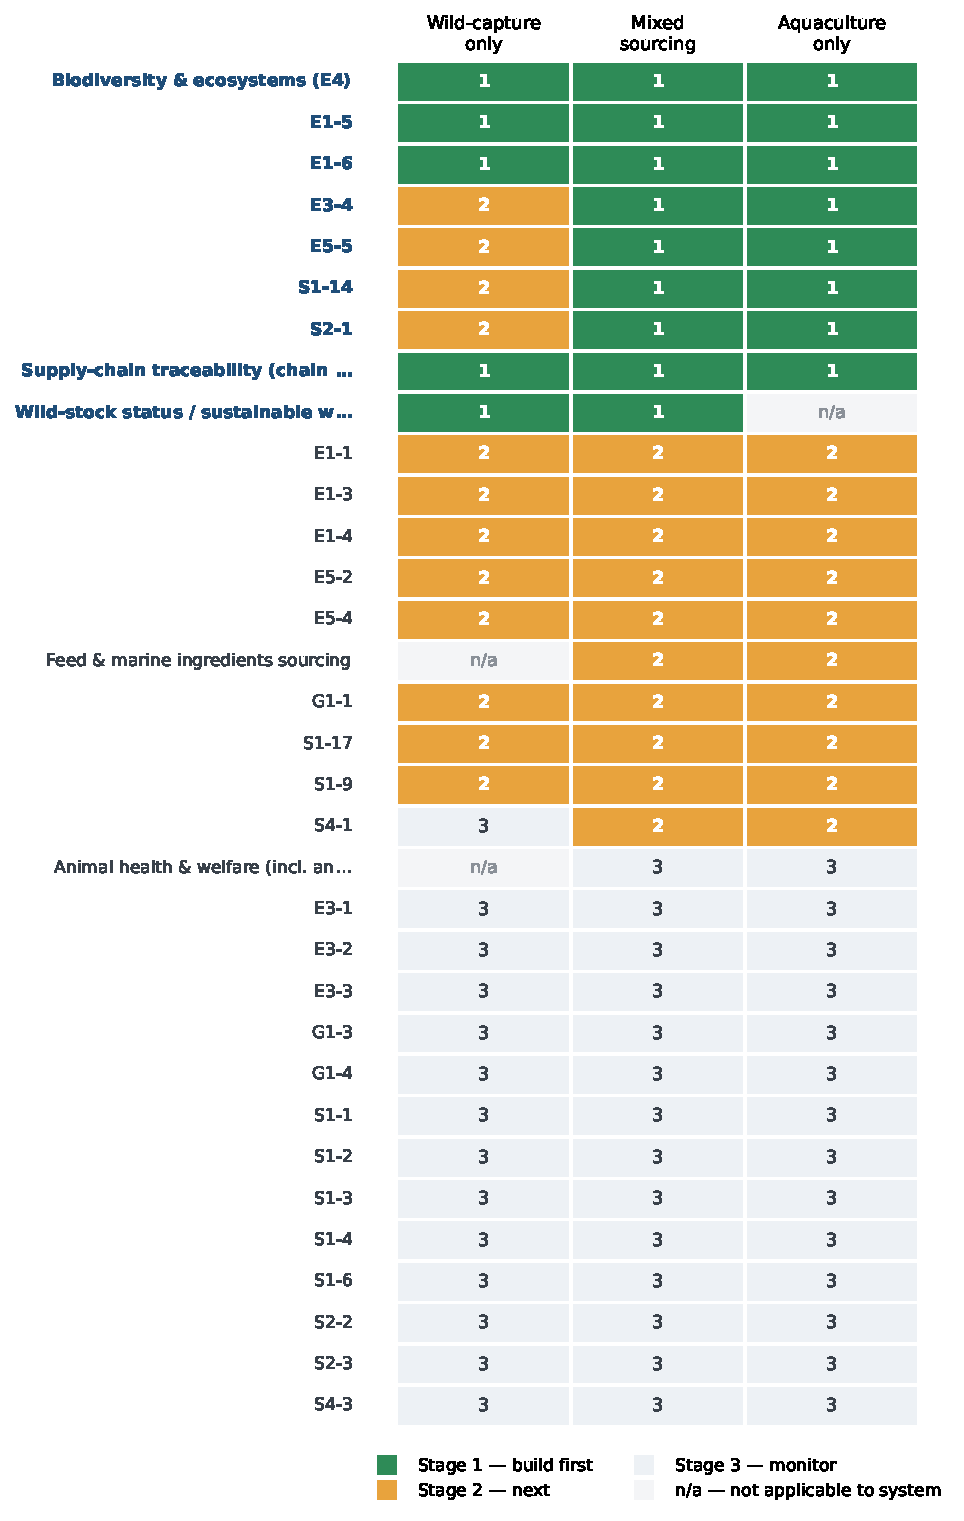
\includegraphics[width=0.56\linewidth]{r_stage_system.pdf}
\caption{First action points by production system. Each topic's stage
(1~=~build first, 2~=~next, 3~=~monitor) under a wild-only, mixed and
aquaculture-only profile; ``--'' marks a topic not applicable to that system. The
four topics that are Stage~1 across all systems form the universal core.}
\label{fig:r-stage-system}
\end{figure}

\FloatBarrier
\subsection{6.8 Step 4: from themes to datapoints, and the diagnostic
tool}\label{cm-datapoints-tool}

\textbf{The build-first data layer.} The staging returns priority \emph{themes};
a firm still needs to know which \emph{datapoints} to collect for each. A
datapoint layer translates every priority theme into the specific data the firm
must produce. The ESRS topical requirements decompose into their constituent
datapoints (the ESRS datapoint catalogue under Commission Delegated Regulation
(EU) 2023/2772): the 26 DR-level Stage rows resolve to 356 official datapoints
and the two topic-level rows (E4, S4) to a further 152. For each theme the
\emph{proportionate} subset - the realistic starting point for a smaller
firm - is identified through the VSME-to-ESRS crosswalk (\nameref{app:crosswalk}),
which maps every VSME Basic and Comprehensive module datapoint to the ESRS
disclosure requirement it is thematically closest to and flags whether it is
realistically self-reportable without external verification.
The crosswalk operates at disclosure-requirement level, not at official-datapoint
level: no ESRS datapoint is itself tagged as a starting point, but a VSME
datapoint mapped onto a theme's requirement shows that a lighter, self-assessable
version of that requirement exists. Applied to the Stage-1 set, five of the seven
ESRS-anchored topics have solid VSME coverage - energy, GHG emissions, water,
waste, and health and safety. Biodiversity is covered only partially, and
value-chain workers (S2-1) not at all. This confirms at datapoint resolution the
gap already identified in \nameref{app:esrs-mapping}. The four seafood-specific
themes have no ESRS requirement and are sourced from GRI~13, so they correctly
have no VSME entry either.

\textbf{The enabling layer.} Knowing which datapoints to collect is not the same
as knowing how to produce them. Each topic therefore also carries the enabling
instruments that generate its data - the GHG Protocol for emissions accounting,
GDST for traceability, ISO~14001 for environmental management. These are methods
and management systems rather than disclosure demands, which is why they are held
outside the demand sums (Section~6.3). Eight of the nine Stage-1 topics
carry at least one enabling instrument; biodiversity is the exception, with no
established method specific enough to name, which is consistent with its partial
VSME coverage and with its being the topic where demand most clearly outruns
practice (Section~7.1).

Each \emph{topic} (not datapoint) carries the count of stakeholder demands it
serves, taken from the matrix (Section~6.4). This makes the reuse
explicit: a single topic typically satisfies several frameworks at once. Because
both the ESRS and the VSME are under active Omnibus revision, the layer is a dated
snapshot documented with its sources.

\textbf{The diagnostic tool.} The staging logic is operationalised as a working
prototype for an individual SME. The tool takes two inputs the firm can supply
directly. The first is a short reporting-posture self-assessment of five to eight
items: whether it has a formal sustainability strategy, a dedicated function or
role, externally or internally initiated reporting, voluntary commitments such as
SBTi-aligned targets, and disclosure data that is reusable across requests. The
second is its production profile - wild, aquaculture or mixed, and size band. It
returns the firm's Stage-1 build-first topics filtered to that profile, and the
datapoint layer beneath them. This is the core of the diagnostic: it turns the
general staging into a personalised shortlist.

Two extensions are designed but not yet built into the prototype, and are described
here as the intended next increment. The first is a \emph{stakeholder-pressure
input}: the firm would identify which customers, certifications and investors are
actively asking, so the shortlist could be narrowed further to the topics where its
\emph{actual} demand and the convergent topics coincide. The second is a fully
automated \emph{staged roadmap} sequencing Stage~1~$\rightarrow$~2~$\rightarrow$~3
against the firm's posture and resourcing. Positioning on the reactive-to-proactive
spectrum is left to the self-assessment, on the basis that posture is a behavioural
rather than a measurable categorical state that the firm is best placed to judge.

\FloatBarrier
\subsection{6.9 Step 4 continued: worked case and
validation}\label{cm-worked-case}
% Scoping note: validating the diagnostic against a named real firm is
% deliberately left as a specified next step rather than attempted within
% this thesis -- a considered scope decision, not an oversight. Confirmed
% with Ruben (2026-07-24) to keep this framing given the send timeline.

\textbf{Worked case: scope and next step.} Validating the diagnostic against
a real firm's public disclosures is the natural empirical next step after
this thesis, and is deliberately scoped here as specified future work rather
than attempted under this thesis's time constraints. The design is specified
precisely enough to be immediately actionable: a representative European
mid-sized seafood-processing SME (50--250 employees, primarily a B2B
supplier to large EU retailers) would be profiled using only material the
firm has itself published - its sustainability report, certification
listings, and customer and product information - so the exercise depends
on no privileged access and is fully reproducible by a future researcher or
practitioner without a partner firm's cooperation. The diagnostic would be
run on that profile, and its output examined for correspondence to the
firm's observable position: whether it locates the firm's posture plausibly,
and whether the topics it flags as build-first match the demands the firm is
visibly subject to. By design the case is singular and \emph{formative rather
than confirmatory} - a usability demonstration of the diagnostic, not a
test of the underlying empirical claims about the cohort or the
cross-framework demand pattern - and no generalisation beyond it would be
claimed. Practitioner validation of the diagnosis with the firm itself is a
further, separate step, identified here and left to future work regardless
of whether the worked case is carried out first.

Figure~\ref{fig:tool-screenshot} shows the diagnostic's actual output screen,
illustrating the format this validation step would use. The profile shown sits
within the scoped parameters - mixed wild-plus-aquaculture sourcing, sub-250
employees - rather than belonging to a named firm. Given a production profile,
the tool returns a ranked Stage-1 build-first set and states how much of the
demand environment building it answers. A firm therefore sees not only
\emph{what} to build first but \emph{why that subset}.

\begin{figure}[htbp]
\centering
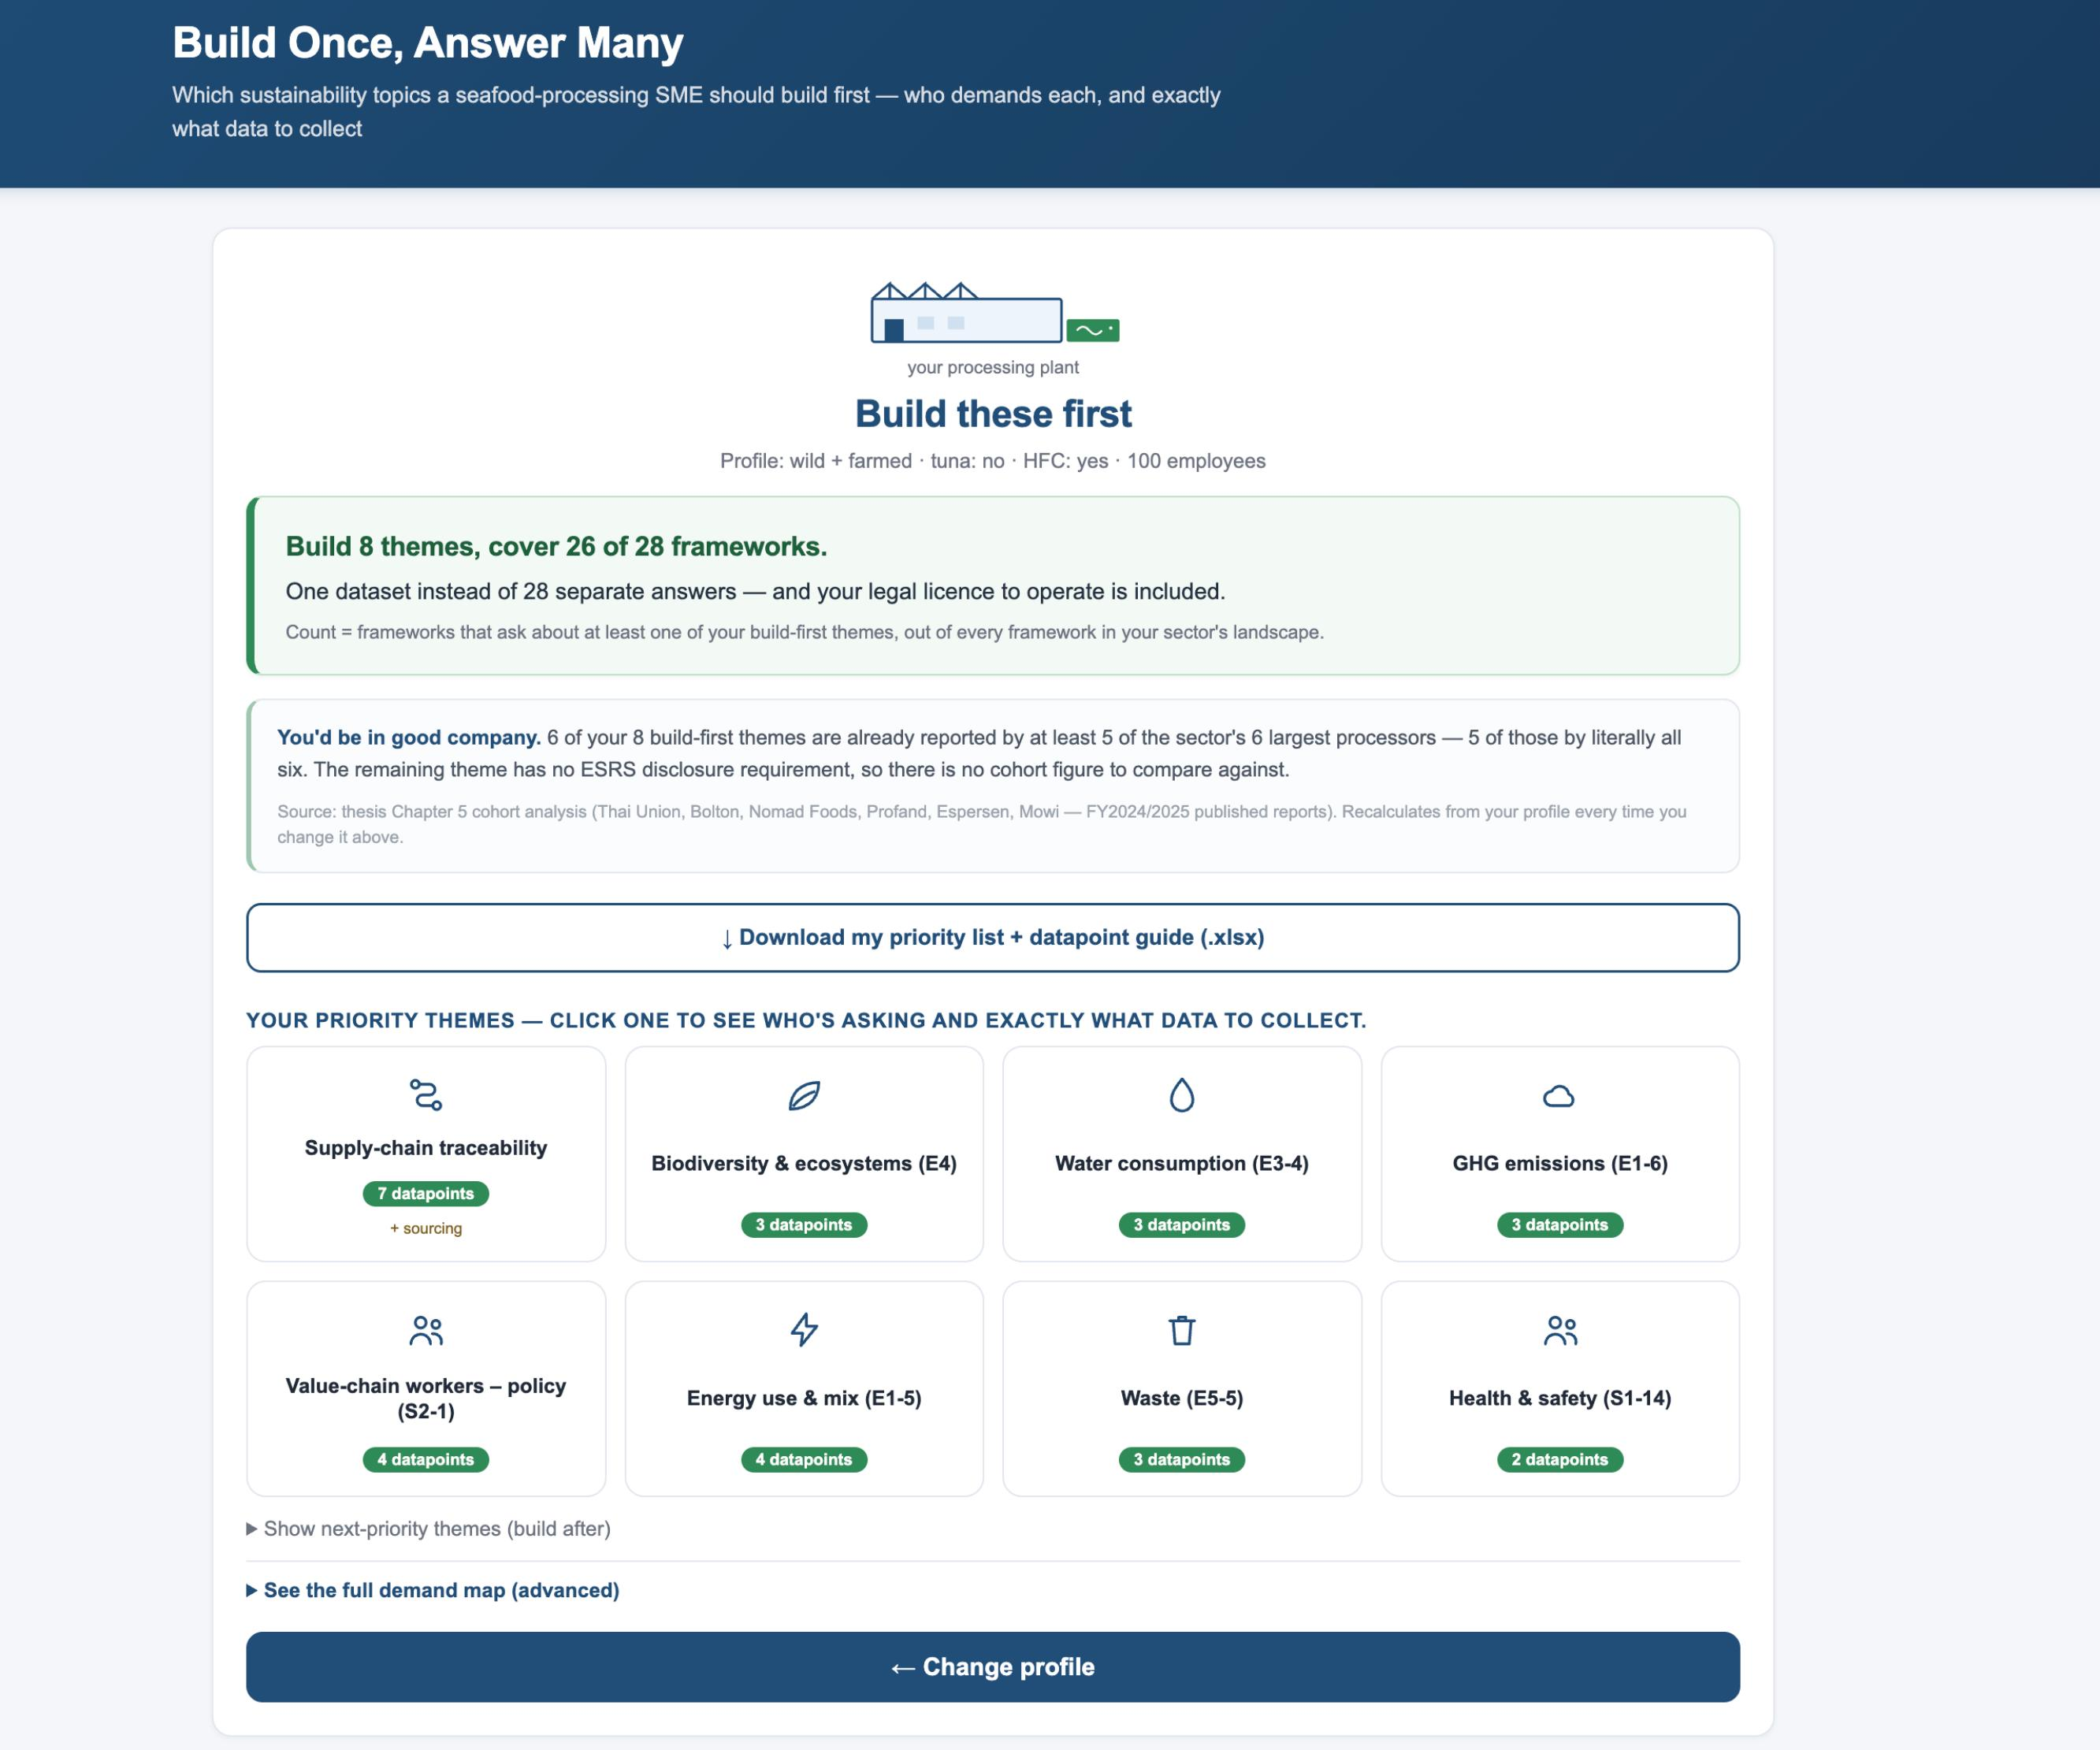
\includegraphics[width=\linewidth]{phase3/tool.jpg}
\caption{The diagnostic tool's output screen: for a given production
profile, it returns the ranked Stage-1 (build-first) themes, the
datapoints each requires, and the share of the sector's demand environment
they jointly answer. This is the operational form the
staging logic of Section~6.4 takes for an individual firm. The mixed profile
shown returns nine Stage-1 topics but eight tiles, because the tool presents
wild-stock sourcing within supply-chain traceability - the two are evidenced
by one set of chain-of-custody data.}
\label{fig:tool-screenshot}
\end{figure}

\textbf{Validation of the mapping and the mechanism.} Both the demand mapping and
the capability-sharing claim beneath it are substantiated from documents, so that
credibility rests on independently inspectable evidence rather than on any single
informant.

The \emph{descriptive} claim is that the ecosystem can be organised exhaustively
and unambiguously by the necessity, domain and source axes. Its test is the
completeness of the classification itself, every instrument placed and every
placement reasoned. The classification has also been submitted to the
sustainability leads at the cohort firms for member checking (Lincoln \& Guba,
1985); that corroboration is outstanding at the time of writing.

The \emph{explanatory} claim is that capabilities are shared across requirements,
so that investment compelled by a lower-tier requirement subsidises higher-tier
disclosure. This is substantiated through an \emph{input-overlap analysis}: for
each shared capability, the inputs the drawing instruments require are read
directly from their published specifications. MSC chain-of-custody, the GDST
standard and ESRS value-chain disclosure all draw on the same body of lot-level
traceability data - shared inputs that are document-verifiable rather than
self-reported.

The evidence is therefore \emph{consistent with} the capability-sharing mechanism;
it does not prove a causal relationship. Establishing that would take retrospective
practitioner testimony on whether capability built for a mandatory requirement
reduced the effort of later disclosures. That is the natural next stage, and is
left to future work.

\medskip
The implications for seafood SMEs and for EU disclosure policy are drawn out
in the discussion that follows.

\FloatBarrier




\section{7. Discussion and conclusion}\label{discussion}

\subsection{7.1 What the four steps establish
together}\label{discussion-summary}

The four steps answer one question, not four unrelated ones. Step~1 catalogued 49
instruments acting on a European seafood-processing SME and found they reach the
firm through only four stakeholder channels. Step~2 found the sector's six most
advanced reporters cover between 33 and 60 of the 70 screened ESRS disclosure
requirements and converge on a 13-requirement core that survives every robustness
cut applied to it. Step~3 crossed the two: of 1{,}023 instrument-by-topic cells only
188 (18\%) carry demand at all, and that sparse demand concentrates on a Stage-1
set of nine topics for a mixed-sourcing firm, which between them touch a topic
asked about by 26 of the 30 frameworks active in the sector.\footnote{Counting a
framework whether it legally binds the firm or is a certification the firm may
choose to pursue.} Step~4 turned that into a diagnostic a firm can apply to its own
profile (\nameref{cm-datapoints-tool}).

The answer to the organising question follows directly. A resource-constrained
seafood-processing SME does not face an undifferentiated wall of demand. It faces a
small, identifiable, cross-cutting core, surrounded by a long tail of narrower
requirements. What to build first is nameable, and now toolable.

A closer look at where Step~2's and Step~3's two ``cores'' agree, and where
they do not, sharpens this picture further. Of Step~3's four-topic universal
Stage-1 core - the topics a firm should build first irrespective of
production system - two (energy consumption, E1-5, and gross GHG
emissions, E1-6) sit squarely inside Step~2's 13-requirement reported
baseline: the sector's mature reporters already treat them as standard
practice, and the cross-stakeholder demand structure independently confirms
they are exactly where demand concentrates. The other two, however, are not
yet part of that reported baseline: biodiversity (E4) only clears Step~2's
near-universal threshold through the topic-level union rule rather than as a
core requirement outright, and supply-chain traceability has no ESRS home at
all and enters Step~3's rows only as a seafood-specific addition
(Section~6.2). Conversely, water, governance and workforce topics anchor
Step~2's reported baseline without appearing in Step~3's cross-system
core. This is not a contradiction between the two steps but a finding in its
own right. Reporting practice and cross-stakeholder demand agree that climate
accounting is foundational. They diverge in two directions after that.
Reporting \emph{lags} demand on biodiversity and traceability, the newer and
harder-to-operationalise topics. It runs \emph{ahead} of demand on water,
governance and workforce. The likely reason for the second gap is that those
topics are anchored by requirements specific to particular sourcing models
(Section~6.7), which a cross-system view averages away.

\subsection{7.2 Reading the findings through the conceptual
framework}\label{discussion-theory}

Chapter~2 set out three lenses for reading multi-stakeholder demand. Each now
returns something the findings sharpen, and in one case something the findings
complicate.

\textbf{Stakeholder salience: transmission, not just attributes.} Mitchell, Agle
and Wood (1997) explain how firms triage competing claims by the power, legitimacy
and urgency a claimant holds. Applied directly to an SME, that account predicts
the firm attends most to whoever can most immediately damage it. The
narrow-law/broad-cascade finding (Section~6.6) suggests the mechanism is more
indirect than that. The instruments generating most of the demand a small
processor experiences - CSRD, CSDDD, SFDR - are not ones for which the processor
is a claimant's target at all; they bind its \emph{customers}, and reach the
processor as transmitted questionnaires. The salient party, in the sense the
theory intends, is the retailer. But the substance of what is asked is set by a
regulator with no direct relationship to the processor whatsoever.

Salience, on this evidence, is not only a property of the claimant a firm faces.
It is a property of the \emph{chain} through which an obligation travels: a
high-power regulator acting on a high-power customer generates more demand on a
small supplier than a regulator binding that supplier directly. This is why
Chapter~4 codes instruments to the channel through which they arrive rather than
to their nominal issuer, and it is a refinement the seafood case makes visible
because the sector's SMEs sit almost entirely below the CSRD threshold while
selling almost entirely to firms above it.

\textbf{Institutional isomorphism: which mechanism?} The 13-requirement universal
core (Section~5.5) is a convergence result, and DiMaggio and Powell (1983) offer
three candidate explanations. Coercive isomorphism fits poorly on its own: the six
firms report under different regimes, three under the ESRS and three under the GRI
at two different application levels (Section~5.3), so no single mandate compels the
overlap. That leaves the mimetic and normative mechanisms, which the evidence
cannot fully separate. What it can show is that the core survives every cut applied
to it - by threshold, by cohort composition, by EU versus non-EU membership
(Section~5.7) - which is what one would expect of a settled professional norm and
less of what one would expect from firms imitating a single visible leader.

The finding that would distinguish the two is not available here and is worth
naming as such: mimetic pressure predicts a diffusion \emph{sequence}, with later
adopters following earlier ones topic by topic, whereas a normative account
predicts firms arriving at the same core independently through shared professional
and assurance practice. A longer panel than two years would let a future study
adjudicate this directly.

\textbf{The resource-based view, and where it cuts against the argument.} The
capability-sharing claim rests on the resource-based view and its
dynamic-capabilities extension (Barney, 1991; Teece, 2007): structured data, once
built, is redeployable across many uses at low marginal cost. The redeployability
half holds, and the input-overlap analysis (Section~6.9) documents it.

Barney's other criteria do not, and this should be stated plainly rather than
passed over. A capability confers sustained competitive advantage only if it is
also rare and costly to imitate. Lot-level traceability data is neither. Every
processor can build it, the enabling instruments that produce it are public
(Section~6.8), and the sector's leading firms have already built it. On a strict
reading of Barney, the build-first core is not a source of advantage at all: it is
the price of remaining in the market.

That is not a defeat for the argument; it changes what the argument claims. The
return on building the convergent core is not differentiation but \emph{efficiency
and access} - the same licence to operate and to sell obtained at materially lower
cost than answering each demand separately, which is the compound return Chapter~2
describes and Chapter~6 measures. Advantage, if it exists, sits one level up: in
the organisational capability to identify which data to build and to reuse it
quickly, which is a dynamic capability in Teece's sense rather than a resource in
Barney's. The diagnostic developed here is best understood as an attempt to lower
the cost of acquiring precisely that capability for firms that cannot develop it
through experience alone.

This is the precise sense in which compliance obligations become strategic
advantage, and it is worth stating exactly because the phrase invites a stronger
reading than the evidence supports. The obligations themselves confer nothing:
every competitor faces them, and every competitor can meet them. What is open to
advantage is the \emph{manner} of meeting them - once, deliberately, and in a form
that also serves the next demand. The return is realised as cost avoided and
access retained rather than as a position rivals cannot occupy, and it accrues to
the firm that builds the underlying capability earliest rather than to the one
that holds any particular dataset.

\subsection{7.3 Contribution to seafood-processing
SMEs}\label{discussion-sme-contribution}

For seafood-processing SMEs, the contribution is the Stage-1 build-first set
itself and the datapoint layer beneath it (Section~6.8), not as an abstract
finding but as a concrete starting list: energy and GHG accounting (E1-5,
E1-6), water (E3-4), biodiversity (E4), supply-chain traceability, and - for
mixed and aquaculture profiles - waste, occupational health and safety, and
value-chain-worker policy.
Building these first is a \emph{sequencing} argument, not a completeness one:
because even the cohort's best-resourced reporters leave roughly a quarter of
the screened requirements uncovered (Section~5.4), completeness is the wrong
target for a smaller firm, and the diagnostic's contribution is to say which
subset to prioritise rather than to promise a shortcut to full compliance.

The diagnostic tool (Section~6.8) turns this from a static finding into a
usable instrument: a firm supplies a short self-assessment and its production
profile, and receives its own filtered Stage-1 set and datapoint layer rather
than the sector-wide one. This matters because the build-first set is not
identical across production systems (Section~6.7), and the reason is a
genuine feature of the current instrument landscape rather than an artefact
of how the tool is built: the catalogue carries three aquaculture
certifications (ASC, BAP, GLOBALG.A.P.) against only two for wild-capture
(MSC, Friend of the Sea). For a shared topic such as water or waste, a
wild-capture-only firm loses the extra breadth those additional aquaculture
certifications would have contributed, so the topic's volume score falls
below the Stage-1 cut even though its \emph{convergence} - how many of the
four stakeholder channels ask about it - is unchanged. A wild-capture-only
firm therefore has a narrower Stage-1 set not because the tool treats it
differently in principle, but because fewer certifications currently exist
for its sourcing model; a generic, one-size-fits-all list would consequently
over- or under-state what any individual firm actually needs.

The diagnostic's output format is illustrated in Section~6.9
(Figure~\ref{fig:tool-screenshot}); a worked case applying it end to end to a
specific, publicly reconstructable firm and checking its flagged Stage-1
topics against that firm's actual disclosures is the natural closing
demonstration for this section, once that case is identified.

\subsection{7.4 Academic contribution}\label{discussion-academic}

The thesis makes four contributions to the literatures reviewed in
Chapter~2. First, it supplies what that review found missing (Section~2.1,
``the gap''): a systematic mapping of cross-stakeholder disclosure demand at
sector level, built on the defined 0/1/2 coverage scale set out in
Section~6.3 - not covered, touched, or bindingly required - rather than
an impressionistic count of ``how many frameworks'' apply.

Second, the narrow-law, broad-cascade finding (Section~6.6): direct regulation on
the processor is targeted and lean, while breadth is transmitted down the value
chain from a handful of horizontal instruments. To the author's knowledge this has
not been demonstrated empirically for the sector before, and it reframes the
burden question - the wall of demand a small firm experiences is substantially a
cascade effect of large-firm regulation (CSRD, CSDDD, SFDR) rather than direct
over-regulation of the SME itself. Section~7.2 draws out what this implies for
stakeholder-salience theory.

Third, the thesis extends the reactive--proactive and maturity literatures
(Baumgartner \& Ebner, 2010; Sharma \& Vredenburg, 1998; Torugsa, O'Donohue \&
Hecker, 2013) - which describe the posture and its performance consequences
but say little about how the external structure of demand enables or blocks
the transition - with a diagnostic-tool operationalisation: a way of making
the ``build shared capability'' prescription concrete for a named sector,
rather than leaving it at the level of strategic recommendation.

Fourth, the cohort analysis (Chapter~5) is itself a methodological
contribution to the maturity literature: it demonstrates that a sector's
disclosure frontier and its universal core can be derived directly from
mature firms' own reporting practice, cross-validated for robustness against
threshold choice, cohort composition and reporting year (Section~5.7), rather
than assumed from theory or asserted by expert judgement alone.

\subsection{7.5 Implications for EU disclosure
policy}\label{discussion-policy}

The findings speak directly to the live Omnibus simplification debate, and
in one respect more concretely than a debate still in progress: as detailed
below, the direction this thesis anticipated is now a matter of adopted
record rather than proposal. Three points stand out.

First, the narrow-law/broad-cascade finding (Section~6.6)
locates the policy lever precisely: because the SME's burden originates
overwhelmingly in the downward cascade of large-firm regulation rather than in
direct sector-specific rules, it is the \emph{coordination and capping} of
that cascade - the explicit aim of the VSME and the Omnibus value-chain
provisions - that would reduce SME burden fastest, more than any further
simplification of direct obligations on the SME itself.

Second, and more speculatively than the other two, the cohort's contracting
disclosure trend (Section~5.7) is worth flagging as a
direction to watch rather than a conclusion this thesis can support: coverage
fell slightly from 2024 to 2025 for the three cohort firms with both years,
in the same direction as the decline in declared materiality documented
across 241 large listed EU companies (Nahrstedt, 2026). Three firms over two years cannot establish whether
this reflects firms reading the Omnibus's relief as a floor or a ceiling - that would need a far larger panel than this thesis's cohort provides - but
the fact that an independent, much larger sample moves the same way is reason
enough to flag the question for the re-anchored analysis in Section~7.7
rather than to answer it here.

Third, the sector's own blind spots and the revision's own priorities turn
out to point in \emph{opposite} directions, which is a sharper finding than
either alone. The requirements that phase in slowest under the Omnibus
timeline - anticipated financial effects and pollution disclosure - are
exactly the cohort's collective blind spot (Section~5.6); simplification
is, for now, deferring precisely what the sector was not yet disclosing
anyway. Biodiversity runs the other way. It is the topic the demand structure
most clearly flagged as under-reported relative to how widely it is demanded
(Section~7.1), and the revision tightens it rather than easing it: the standards
adopted on 3~July 2026 make biodiversity transition plans mandatory where they
were previously voluntary. Meanwhile the water standard loses roughly 70\% of its
mandatory datapoints, the deepest cut of any topical area - and water was already
part of the cohort's reported baseline (Section~5.5). The revision is
therefore easing what mature practice had already absorbed and tightening what
this thesis found demand was outpacing practice on. That is consistent with the
Chapter~6 demand structure rather than a correction of it.

This alignment is no longer only a matter of timeline projection. On 3~July
2026 the European Commission formally adopted the revised ESRS and a new
voluntary reporting standard for smaller companies built on the VSME,
cutting mandatory datapoints by over 60\% and total datapoints by over 70\%
(European Commission, 2026) - the reduction this thesis anticipated
throughout (Section~1.5) is therefore no longer a proposal under debate but
an adopted delegated act, pending only the standard two-to-four-month
European Parliament and Council scrutiny period before it applies. The
adopted standard also formalises the value-chain cap referenced in the
introduction (Section~1.1): CSRD-scoped firms may not require value-chain
partners to supply more than the voluntary standard covers. This does not
change any finding in this thesis, whose cohort and demand-matrix analysis
predate the adoption, but it does mean the policy debate this thesis speaks
to has moved, in the ten days before submission, from live negotiation to
implementation - and it strengthens rather than weakens the case for the
future-work item below: re-anchoring this analysis to the adopted standard
once it takes effect.

Fourth, the case this thesis makes for building VSME-aligned capability rests
on an assumption worth testing against independent evidence: that customers,
banks and investors will actually treat a VSME-based disclosure as
sufficient, rather than continuing to ask for more. EFRAG's own market
acceptance survey of preparers and users (EFRAG, 2025) gives this some
support: it finds developing, positive acceptance of the VSME, with
financial institutions and investors expecting its modules to satisfy a
substantial share of the requests they currently address directly to SMEs.
The finding is preliminary, and self-reported to the standard-setter that
designed the VSME, so it should be read as encouraging rather than conclusive.
It nonetheless points the same way as the narrow-law/broad-cascade finding
above. The demand a resource-constrained firm faces is transmitted through a small
number of large channels - customers and financiers - which a proportionate,
standardised disclosure can plausibly satisfy. It is not an open-ended list that
every actor insists on customising.

\subsection{7.6 Limitations}\label{discussion-limitations}

Each step's own limitations are stated where the relevant claims are made
(Sections~5.\emph{x}, 6.7, 7.\emph{x}); four apply to the thesis as a whole and
are drawn together here rather than left scattered.

\textbf{Small, purposive samples throughout.} The cohort (N=6) and the demand
matrix's instrument catalogue are both purposive constructions - an
upper-bound proxy and a comprehensiveness claim respectively - not
statistical samples, so no claim of population-level representativeness is
made anywhere in the thesis. The robustness checks in the
Section~5.7 section substitute cross-validation for
statistical inference; they cannot substitute for it.

\textbf{Analyst judgement in the coding.} The GRI-to-ESRS mapping
(Section~5.3), the per-cell demand scoring (Section~6.3) and the
necessity/domain classification (Section~4.1) all rest on a single analyst's
documented judgement, checked against defined criteria and logged for audit
but not independently double-coded. The member-checking review submitted to the
cohort firms (Section~4, Validation) is a corroborating step, not a formal
inter-rater-reliability test, and at the time of writing it is still outstanding.
A second-coder check remains future work (Section~7.7). One firm's review has
since returned and is reflected in Section~5.3.

\textbf{What the framework bridge cannot carry.} Cohort coverage is coded from
each firm's own framework index, and three of the six firms are indexed under the
GRI Standards. Two consequences follow, both set out in Section~5.3. A firm whose
index is selective scores below what its report body contains, which is a
question of indexing practice. More structurally, 14 of the 70 topical
disclosure requirements have no counterpart anywhere in the GRI-ESRS
interoperability index, so no GRI-indexed firm can score them at all; those 14
can be reported by at most three of the six firms and can never enter the
universal core or the near-universal set. The effect on the findings is bounded
and small. None of the 14 could reach six of six even if every GRI-indexed firm
reported it in full, because each already lacks at least one ESRS-native
reporter, so the universal core of 13 is exact rather than a floor. Only two,
E1-1 and S2-5, could in principle reach five of six, placing an upper bound of 28
on the near-universal set of 26. The limitation is real, and it does distort the
firm-by-firm coverage comparison, but neither headline result rests on the
unmeasured cells.

\textbf{The sector-material row set is curated, not exhaustive.} The four
sector-material rows (\nameref{cm-matrix-build}) were chosen because GRI~13
asks for genuinely different operational data - species, volumes, stock
status - that no ESRS or generic GRI disclosure asks for at all. GRI~13
contains other sector-specific disclosures that were judged, but not
included, because they refine an already-covered topic rather than open a
new one: certified-volume reporting under food safety (13.10), and
nationality/migrant-status breakdowns under non-discrimination (13.15), for
example, sit inside topics the cohort already reports on. One further
candidate follows the same logic already used for feed and animal welfare
above and was a closer call: ASC's conversion-free-sourcing criterion, which
reaches a processor exactly as feed and welfare demand does, as a
certification precondition rather than direct operational reporting. It is
left out of the four rows here for scope, not because the logic doesn't
apply - extending the sector-material row set on that same
certification-precondition basis is a natural next check, not a finding
this thesis is confident closes the question.

\textbf{A 2024--2025 snapshot of a moving target.} The ESRS, the VSME and the
Omnibus simplification were all under active revision throughout this
analysis, and the revised ESRS and a new VSME-based voluntary standard were
formally adopted only in the final weeks before submission (3~July 2026;
Section~7.5), with the standard two-to-four-month Parliament and Council
scrutiny period still to run. The coverage figures, the demand-matrix scores
and the year-over-year comparison in the Section~5.7 section
are dated to the 2024--2025 window that precedes this adoption and will need
re-anchoring once the revised standard actually takes effect. Checked against
EFRAG's draft revised standards, that re-anchoring is a matter of translation
rather than revision. Every disclosure requirement in the 13-requirement
universal core (Section~5.5) and in the four-topic Stage-1 core common
to all production systems (Section~6.7) survives in substance; none was deleted.
Most simply carry a different DR code. Several standards gained new upfront
requirements, chiefly on risk identification and resilience, which shifted
everything after them down by one to three positions - energy consumption moves
from E1-5 to E1-7, GHG emissions from E1-6 to E1-8. The full old-to-new code
mapping, cross-referenced against the VSME, is given in
\nameref{app:esrs-mapping}.

\textbf{One formative, not confirmatory, worked case.} The diagnostic's
usability is demonstrated on a single public case (Section~6.9); no claim of
generalisation beyond that case is made, and practitioner validation with a
firm willing to share non-public information is explicitly left to future
work.

\subsection{7.7 Future work}\label{discussion-future-work}

Several extensions are flagged at the point they arise in Chapters~4--6;
gathered here, they form a natural research agenda. \emph{Practitioner
validation}: running the diagnostic with a firm willing to share internal
data beyond its public disclosures, to test the worked case's formative
finding against a confirmatory one (Section~6.9). \emph{Reliability}: a
second-coder pass on the GRI-ESRS mapping and the demand-matrix scoring, to
convert the current documented-judgement audit trail into a measured
inter-rater agreement (Section~5.3 and Section~6.3). \emph{Stakeholder-pressure input}:
the tool extension, already scoped but not yet built (Section~6.8), that lets
a firm identify which of its own customers, certifications and investors are
actively asking, narrowing the generic Stage-1 set to the firm's
\emph{actual} demand. \emph{A staged roadmap}: automating the
Stage~1~$\rightarrow$~2~$\rightarrow$~3 sequencing against a firm's posture and
resourcing, rather than leaving that positioning to the self-assessment alone
(Section~6.8). \emph{Re-anchoring to the adopted ESRS revision}: repeating the
cohort and demand-matrix analysis once the standards adopted on 3~July 2026
(Section~7.5) clear Parliamentary and Council scrutiny and take effect, both
to test whether the contracting-disclosure trend
(Section~5.7) persists and to keep the diagnostic's datapoint
layer current against the roughly 70\%-smaller datapoint set.
\emph{Sectoral transfer}: testing whether the build-first core identified here
is seafood-specific or reflects a more general cross-sector pattern, in the
other resource-constrained manufacturing and agri-food SME contexts the
introduction argues the approach should transfer to (Section~1.4).
\emph{From diagnosis to implementation}: this thesis stops at telling a firm
\emph{which} topics to build first; the natural next step is piloting the
framework with actual firms to see how a prioritised topic list translates
into the internal processes, ownership and data infrastructure needed to
build it, and to learn where firms get stuck turning a build-first list into
a working data-collection routine. Beyond validating the diagnostic's
outputs (the practitioner-validation item above), this would test the
thesis's implicit second claim - that naming the right topics is enough to
unblock action - which this thesis has not itself tested.

\subsection{7.8 Conclusion}\label{discussion-conclusion}

This thesis set out to answer where, amid a thicket of overlapping
sustainability demands, a resource-constrained European seafood-processing SME
should begin. Three linked findings answer it. The disclosure ecosystem
acting on such a firm is wide but structured, not undifferentiated
(Chapter~4). The sector's own leading reporters already converge on a
compact, cross-cutting disclosure core, not an ever-expanding one
(Chapter~5). And that empirical core is exactly where cross-stakeholder demand
is most concentrated, so that building it first answers the largest share of
what the firm is actually asked, operationalised here as a diagnostic an
individual firm can apply to its own situation (Chapter~6).

\textbf{What is now known that was not.} Three things. First, the demand a small
processor faces is measurably sparse: 18 per cent of the possible
instrument-by-topic space carries any demand at all, which is what makes
prioritisation coherent rather than arbitrary. Second, the burden originates
overwhelmingly in transmission rather than in direct regulation, so the wall a
small firm experiences is a cascade from large-firm rules and not
over-regulation of small firms themselves. Third, the sector's revealed reporting
baseline and its cross-stakeholder demand structure substantially agree, and where
they diverge - biodiversity and traceability, where demand runs ahead of practice -
they identify precisely the topics a forward-looking firm should build before it
is asked.

\textbf{What remains open.} The diagnostic has not been run with a firm that can
supply internal data, so the claim that naming the right topics unblocks action
remains untested (Section~7.7). The coding rests on a single analyst's documented
judgement, with member checking outstanding at the time of writing. And whether the
convergent core identified here is a seafood phenomenon or a general feature of
resource-constrained manufacturing and agri-food sectors is an empirical question
this thesis frames but does not answer: the \emph{method} transfers by
construction - any sector with a defined disclosure taxonomy, an identifiable set
of leading reporters and a catalogue of instruments can be mapped the same way -
but the \emph{particular} build-first set almost certainly does not.

\textbf{What it means in practice.} For a firm deciding what to do on Monday
morning, the answer is narrower than the literature's usual advice to become
strategic about sustainability. Build energy and greenhouse-gas accounting, water,
biodiversity and supply-chain traceability first, in that order, and build them as
reusable data rather than as answers to whoever asked last. Those four are demanded
across every stakeholder channel and under every production system studied here.
The rest can wait, and knowing what can wait is the scarcer piece of information.

Together these findings turn ``build a reusable sustainability-data capability''
from a strategic aspiration into a named, sequenced and practically actionable
starting list - the missing view this thesis set out to supply.

\section*{Declaration on the use of generative AI}
\addcontentsline{toc}{section}{Declaration on the use of generative AI}

Generative AI tools were used in the preparation of this thesis, under the
author's direction and review throughout. They assisted with language and
presentation - drafting, rewriting for clarity and concision, and copy-editing -
and with computational work, including scripting the extraction of data from the
source workbooks, generating the figures from that data, and checking the
numerical claims in the text against the underlying files.

The research design, the coding decisions, the analysis and the interpretation of
the results are the author's own, as is the responsibility for any errors that
remain.

% ===== References — generated from BIB.rtf (Zotero export). =====
% RUBEN: the 10 originally-missing inline cites (Adams, Barney, EFRAG, ISO,
%   Jabareen, Lincoln, Philips, Russo, Teece, Yin) are now resolved as follows,
%   each verified as a real, existing source before being added below:
%   - Adams & Abhayawansa (2022) -- kept ONLY for the ratings-vs-standards
%     sentence at main.tex:1259. %CL: I confirmed this paper exists and is on
%     sustainability-reporting harmonisation, but could not verify from the
%     abstract alone that it makes this specific ratings/standards distinction
%     -- please sanity-check the page before sending to reviewers. The OTHER
%     Adams & Abhayawansa use (main.tex:414, paired with Christensen/Hail/Leuz)
%     was already flagged by you as inaccurate; I replaced it with Afolabi, Ram
%     & Rimmel (2022), whose title is literally about this harmonisation arena.
%   - Barney (1991), Jabareen (2009), Lincoln & Guba (1985), Russo & Fouts
%     (1997), Teece (2007), Yin (2018): standard, unambiguous, real citations --
%     added below with full details.
%   - Philips (2025): verified against Philips' own "Beyond Auditing" brochure --
%     the exact wording quoted in main.tex ("audit fatigue", "quick fix
%     mentality") is a direct quote from that PDF, dated 2025.
%   - EFRAG: already resolved in an earlier pass (see GRI/EFRAG entries below).
%   - ISO: appears in the text only as inline standard names (ISO 14001, 45001,
%     50001) and in the abbreviations list, never as a parenthetical "(ISO,
%     YYYY)" citation -- so there is nothing to fix in-text. Left unadded here;
%     say the word if you'd like formal standard citations added anyway.
%   All of the above still need to be added to Zotero and this file re-exported
%   once you confirm the flags above.
\phantomsection
\addcontentsline{toc}{section}{References}
\section*{References}
\begingroup
\setlength{\parindent}{0pt}\setlength{\parskip}{6pt}\small
\everypar{\hangindent=1.5em\hangafter=1}

Adams, Carol A., and Subhash Abhayawansa. ``Connecting the COVID-19 Pandemic, Environmental, Social and Governance (ESG) Investing and Calls for `Harmonisation' of Sustainability Reporting.'' \emph{Critical Perspectives on Accounting} 82 (2022): 102309. https://doi.org/10.1016/j.cpa.2021.102309. % %CL: see banner note above -- kept for the ratings-vs-standards sentence at main.tex:1259 only; please sanity-check the page. Add to Zotero and re-export.

Afolabi, Hammed, Ronita Ram, and Gunnar Rimmel. ``Harmonization of Sustainability Reporting Regulation: Analysis of a Contested Arena.'' \emph{Sustainability} 14, no. 9 (2022): 5517. https://doi.org/10.3390/su14095517. % %CL: replaces the previously-inaccurate Adams/Christensen pairing at main.tex:414; please add to Zotero and re-export.

Ahmad, Khursheed, Maria Grazia Marchesano, Valentina Popolo, Roberto Revetria, and Anastasiia Rozhok. ``Development of a European Sustainability Reporting Standards Compliant Sustainability Assessment Framework for Manufacturing Organisations Using Analytic Hierarchy Process.'' \emph{Sustainability} 17, no. 11 (2025): 4772. https://doi.org/10.3390/su17114772.

Ashurst. ``European Commission Consults on Revised ESRS and Sustainability Reporting Standard for Voluntary Use.'' Accessed May 13, 2026. https://www.ashurst.com/en/insights/european-commission-consults-on-revised-esrs-and-sustainability-reporting-standard-for-voluntary-use/.

Barclay, Kate, and Alice Miller. ``The Sustainable Seafood Movement Is a Governance Concert, with the Audience Playing a Key Role.'' \emph{Sustainability} 10, no. 1 (2018): 180. https://doi.org/10.3390/su10010180.

Barney, Jay. ``Firm Resources and Sustained Competitive Advantage.'' \emph{Journal of Management} 17, no. 1 (1991): 99--120. https://doi.org/10.1177/014920639101700108. % %CL: please add to Zotero and re-export.

Bataleblu, Ali Asghar, Erwin Rauch, David S. Cochran, and Dominik T. Matt. ``Impact of European Sustainability Reporting Standards Guidelines on the Design of Sustainable Factories and Manufacturing Systems.'' In \emph{Advances in Manufacturing IV}, edited by Adam Hamrol, Marta Grabowska, and Marcin Hinz. Lecture Notes in Mechanical Engineering. Springer Nature Switzerland, 2024. https://doi.org/10.1007/978-3-031-56474-1\_18.

Battisti, Martina, and Martin Perry. ``Walking the Talk? Environmental Responsibility from the Perspective of Small-Business Owners.'' \emph{Corporate Social Responsibility and Environmental Management} 18, no. 3 (2011): 172--85. https://doi.org/10.1002/csr.266.

Baumgartner, Rupert J., and Daniela Ebner. ``Corporate Sustainability Strategies: Sustainability Profiles and Maturity Levels.'' \emph{Sustainable Development} 18, no. 2 (2010): 76--89. https://doi.org/10.1002/sd.447.

Bolton Group. \emph{Sustainability Report 2024}. 2025. https://www.bolton.com/sites/default/files/2025-04/bolton-sustainability-report\_2024.pdf. % %CL: added as cohort-firm corroboration for the wild-stock/traceability sector-material rows (Ch7); please add to Zotero and re-export.

Bush, Simon, and Peter Oosterveer. \emph{Governing Sustainable Seafood}. Routledge, 2019. https://doi.org/10.4324/9781315780429.

Chan, Ricky Y. K., Jennifer W. M. Lai, and Namwoon Kim. ``Strategic Motives and Performance Implications of Proactive versus Reactive Environmental Strategies in Corporate Sustainable Development.'' \emph{Business Strategy and the Environment} 31, no. 5 (2022): 2127--42. https://doi.org/10.1002/bse.3011.

Cöster, Mathias, Gunnar Dahlin, and Raine Isaksson. ``Are They Reporting the Right Thing and Are They Doing It Right?---A Measurement Maturity Grid for Evaluation of Sustainability Reports.'' \emph{Sustainability} 12, no. 24 (2020): 10393. https://doi.org/10.3390/su122410393.

CSR Tools. ``VSME-Nachhaltigkeitsbericht: Effizientes Mapping der ESRS-Themen.'' 2024. https://csrtools.eu. % %CL: added for Appendix E (VSME-ESRS crosswalk); please add to Zotero and re-export so this isn't lost on the next regeneration.

DiMaggio, Paul J., and Walter W. Powell. ``The Iron Cage Revisited: Institutional Isomorphism and Collective Rationality in Organizational Fields.'' \emph{American Sociological Review} 48, no. 2 (1983): 147--60. https://doi.org/10.2307/2095101.

Dinh, Tami, Anna Husmann, and Gaia Melloni. ``Corporate Sustainability Reporting in Europe: A Scoping Review.'' \emph{Accounting in Europe} 20, no. 1 (2023): 1--29. https://doi.org/10.1080/17449480.2022.2149345.

EFRAG. \emph{Voluntary Sustainability Reporting Standard for Non-Listed Micro-, Small- and Medium-Sized Undertakings (VSME Standard)}. 2024. https://www.efrag.org/sites/default/files/sites/webpublishing/SiteAssets/VSME\%20Standard.pdf. % %CL: added for Appendix E; please add to Zotero (you already had this flagged as a missing EFRAG cite) and re-export.

EFRAG. \emph{VSME Market Acceptance Survey Report}. December 2025. https://www.efrag.org/sites/default/files/media/document/2025-12/VSME\%20Market\%20Acceptance\%20Survey\%20Report.pdf. % %CL: added for Section 8.4's new fourth point; please add to Zotero and re-export.

Espersen. ``Supply Chain Integrity.'' n.d. https://www.espersen.com/sustainability/sustainability/supply-chain-integrity. % %CL: same cohort-corroboration purpose as Bolton above; please add to Zotero.

Fazli, Haleem, Sami Farooq, Cheng Yang, and Brian Vejrum Wæhrens. ``Proactive and Reactive Approaches towards Sustainable Practices in Manufacturing Companies: Emerging Economies Perspective.'' \emph{Sustainability} 15, no. 17 (2023): 12796. https://doi.org/10.3390/su151712796.

``Feedback on Sustainability Reporting Standards: Additional Explanatory Information Regarding the Value Chain Cap - Finance.'' Accessed May 13, 2026. https://finance.ec.europa.eu/news/feedback-sustainability-reporting-standards-additional-explanatory-information-regarding-value-chain-2026-05-06\_en.

Fragidis, Garyfallos, and Triantafyllos Papafloratos. ``An Information Architecture for the European Sustainability Reporting Standards (ESRS).'' \emph{Sustainability} 17, no. 17 (2025): 7675. https://doi.org/10.3390/su17177675.

Himanen, Satu. \emph{Master's Programme in Circular Economy, Master´s Thesis}. 2025.

Global Sustainability Standards Board (GSSB). \emph{GRI 13: Agriculture, Aquaculture and Fishing Sectors 2022}. Global Reporting Initiative, 2022. https://www.globalreporting.org/standards/sector-program/sector-standards/. % %CL: added for Appendix B; please add to Zotero and re-export.

GRI and EFRAG. \emph{GRI--ESRS Interoperability Index}. November 2024. https://www.globalreporting.org/media/qzmoeixv/esrs-gri-interoperability-index-november-2024.pdf. % %CL: this is the actual document Chapter 6 means by "the published GRI-ESRS interoperability mapping" -- I found it was previously cited in the text as bare "(EFRAG, 2024)", which collided with your VSME Standard entry above (also 2024, also EFRAG) -- same in-text citation would have pointed to two different documents. Fixed the in-text cite to "(GRI \& EFRAG, 2024)" and added this as its own entry. Please add to Zotero and re-export.

Hummel, Katrin, and Dominik Jobst. ``An Overview of Corporate Sustainability Reporting Legislation in the European Union.'' \emph{Accounting in Europe} 21, no. 3 (2024): 320--55. https://doi.org/10.1080/17449480.2024.2312145.

Jabareen, Yosef. ``Building a Conceptual Framework: Philosophy, Definitions, and Procedure.'' \emph{International Journal of Qualitative Methods} 8, no. 4 (2009): 49--62. https://doi.org/10.1177/160940690900800406. % %CL: please add to Zotero and re-export.

Kittinger, John N., Louise S. L. Teh, Edward H. Allison, Nathan J. Bennett, Larry B. Crowder, Elena M. Finkbeiner, et al. ``Committing to Socially Responsible Seafood.'' \emph{Science} 356, no. 6341 (2017): 912--13. https://doi.org/10.1126/science.aam9969. % %CL: this citation appeared in Chapter 6 (Thai Union/tuna-scrutiny sentence) with no matching entry in the bibliography at all -- a genuinely undefined reference, now fixed. Please add to Zotero and re-export.

Lincoln, Yvonna S., and Egon G. Guba. \emph{Naturalistic Inquiry}. Beverly Hills, CA: Sage Publications, 1985. % %CL: please add to Zotero and re-export.

Lozano, Rodrigo. ``Are Companies Planning Their Organisational Changes for Corporate Sustainability? An Analysis of Three Case Studies on Resistance to Change and Their Strategies to Overcome It.'' \emph{Corporate Social Responsibility and Environmental Management} 20, no. 5 (2013): 275--95. https://doi.org/10.1002/csr.1290.

Mowi. ``Our Sustainability Certifications.'' n.d. https://mowi.com/sustainability/certifications/. % %CL: cohort-corroboration source; please add to Zotero.

Nahrstedt, Jan. ``Double Materiality in Practice: Evidence from Two Years of CSRD Reporting.'' SSRN working paper, University of Hamburg, 6 May 2026. https://ssrn.com/abstract=6724699.

Nomad Foods. \emph{Sustainability Report 2025}. 2026. https://sustainability.nomadfoods.com/. % %CL: cohort-corroboration source; please add to Zotero.

Nielsen, Christian. ``ESG Reporting and Metrics: From Double Materiality to Key Performance Indicators.'' \emph{Sustainability} 15, no. 24 (2023): 16844. https://doi.org/10.3390/su152416844.

Philips. \emph{Beyond Auditing: Philips' Approach to Supplier Sustainability}. 2025. https://www.philips.com/c-dam/corporate/en\_AA/about/about-us/esg/downloads/beyond-auditing-philips-approach-to-supplier-sustainability.pdf. % %CL: verified -- this is the exact source of the quoted "audit fatigue" / "quick fix mentality" language in main.tex. Please add to Zotero and re-export.

Profand Group. \emph{Sustainability}. n.d. https://profand.com/en/sustainability/. % %CL: cohort-corroboration source; please add to Zotero.

Russo, Michael V., and Paul A. Fouts. ``A Resource-Based Perspective on Corporate Environmental Performance and Profitability.'' \emph{Academy of Management Journal} 40, no. 3 (1997): 534--59. https://doi.org/10.5465/257052. % %CL: please add to Zotero and re-export.

Sharma, Sanjay, and Harrie Vredenburg. ``Proactive Corporate Environmental Strategy and the Development of Competitively Valuable Organizational Capabilities.'' \emph{Strategic Management Journal} 19, no. 8 (1998): 729--53.

Suchman, Mark C. ``Managing Legitimacy: Strategic and Institutional Approaches.'' \emph{The Academy of Management Review} 20, no. 3 (1995): 571--610. https://doi.org/10.2307/258788.

Teece, David J. ``Explicating Dynamic Capabilities: The Nature and Microfoundations of (Sustainable) Enterprise Performance.'' \emph{Strategic Management Journal} 28, no. 13 (2007): 1319--50. https://doi.org/10.1002/smj.640. % %CL: please add to Zotero and re-export.

Thai Union Group PCL. \emph{Sustainability Report 2025}. 2025. https://www.thaiunion.com/uploads/Sustainability\_Report\_2025\_en.pdf. % %CL: cohort-corroboration source; please add to Zotero.

Torugsa, Nuttaneeya Ann, Wayne O'Donohue, and Rob Hecker. ``Proactive CSR: An Empirical Analysis of the Role of Its Economic, Social and Environmental Dimensions on the Association between Capabilities and Performance.'' \emph{Journal of Business Ethics} 115, no. 2 (2013): 383--402. https://doi.org/10.1007/s10551-012-1405-4.

Tugliani, Teresa, Marianna Guareschi, and Filippo Arfini. \emph{Evaluating the Applicability of the European Voluntary Sustainability Reporting Standards for Agrifood Small and Medium-Sized Enterprises}. n.d.

World Wildlife Fund. ``What Are Fishery Improvement Projects?'' Accessed June 4, 2026. https://www.worldwildlife.org/our-work/oceans/improving-fisheries/what-are-fishery-improvement-projects-and-how-do-they-work/.

Yin, Robert K. \emph{Case Study Research and Applications: Design and Methods}. 6th ed. Thousand Oaks, CA: SAGE, 2018. % %CL: please add to Zotero and re-export.

\endgroup

\medskip
{\small\noindent\textbf{Primary sources --- cohort sustainability reports}\par}
% RUBEN: confirm exact titles, editions and years for each firm before sending.
\begingroup
\setlength{\parindent}{0pt}\setlength{\parskip}{6pt}\small
\everypar{\hangindent=1.5em\hangafter=1}

A.~Espersen A/S. \emph{Sustainability Report 2024}. 2025.

Bolton Group (Bolton Food). \emph{Sustainability Report 2024}. 2024.

Mowi ASA. \emph{Annual Report 2025} (integrated). 2025. https://mowi.com/wp-content/uploads/2025/05/Mowi-Annual-Report-2025.pdf.

Nomad Foods Limited. \emph{Sustainability Report 2024}. 2025.

Profand Group. \emph{Sustainability / ESG Report 2024}. 2025.

Thai Union Group PCL. \emph{Sustainable Development Report 2024}. 2024. https://www.thaiunion.com/uploads/sd-report-2024-en.pdf.
\endgroup


\appendix
\clearpage
\section*{Appendices}
\addcontentsline{toc}{section}{Appendices}
\emph{Supplementary material supporting the chapters above.}

\section*{Appendix A - Ecosystem Glossary}\label{app:glossary}
\addcontentsline{toc}{subsection}{Appendix A - Ecosystem Glossary}
\subsection*{A.1 - Foundation and enabling instruments}

Two bands of instruments sit outside the 49-instrument demand landscape catalogued
in Appendix~A.2 and are recorded here instead. \textbf{Tier~0} is the food-safety
and food-law floor every EU seafood processor clears before sustainability strategy
begins: in scope of the firm, out of scope of the sustainability-disclosure
analysis. \textbf{Layer~2} supplies the accounting methods, management systems and
data infrastructure a firm builds capability on; these are excluded from the demand
sums because they do not themselves request a disclosure (Section~6.3).

Snapshot June 2026. EU sustainability law was under active simplification at the
snapshot date; verify against EUR-Lex before citing.

\vspace{6pt}
\noindent\textbf{Tier 0 - Foundation (food integrity)}
\vspace{2pt}

\footnotesize
\begin{xltabular}{\textwidth}{@{} p{4.1cm} X @{}}
\toprule \textbf{Instrument} & \textbf{Objective and role} \\ \midrule \endhead
General Food Law (Reg 178/2002) & General food-safety principles, the
one-step-back / one-step-forward traceability duty, and RASFF. The baseline
food-safety and traceability regime. \\
Hygiene of Foodstuffs (Reg 852/2004) & General hygiene rules for food businesses. \\
Specific Hygiene Rules, Animal Origin (Reg 853/2004) & Hygiene rules for products
of animal origin, including fishery products. \\
Food Information to Consumers (Reg 1169/2011) & Mandatory labelling and consumer
information (ingredients, allergens, provenance) - distinct from the
sustainability claims EmpCo regulates. \\
Food Contact Materials (Reg 1935/2004) & Safety of materials in contact with food;
a packaging-material safety floor, distinct from PPWR's environmental
requirements. \\
Microbiological Criteria (Reg 2073/2005) & Microbiological safety limits for
foodstuffs. \\
Maximum Contaminant Levels (Reg 1881/2006) & Maximum permitted contaminant levels,
relevant to seafood heavy-metal screening. \\
Pesticide Residues (Reg 396/2005) & Maximum residue levels in food and feed,
relevant chiefly to aquaculture feed inputs. \\
REACH (Reg 1907/2006) & Registration and authorisation of chemical substances;
governs processing aids and cleaning agents rather than disclosure. \\
Official Controls Regulation (Reg 2017/625) & Framework for official food-safety
controls and enforcement across the EU. \\
IFS Food & Certifies food-safety and quality-management systems for processors
supplying mainly continental-European retail. Effectively non-negotiable for retail
listing; commercially it functions much like a Tier-2 market licence. \\
BRCGS & Food-safety certification widely required by UK and international
retailers; a near-substitute for IFS Food, buyer choice largely geographic. \\
FSSC 22000 & ISO 22000 plus sector-specific prerequisite programmes; the third
common GFSI-benchmarked option, interchangeable with IFS and BRCGS in most buyer
specifications. \\
GFSI & Benchmarks food-safety schemes for mutual recognition. The reason IFS,
BRCGS and FSSC behave as near-substitutes, and why they are not counted as three
independent demands. \\
\bottomrule
\end{xltabular}
\normalsize

\vspace{6pt}
\noindent\textbf{Layer 2 - Enablement / methodology layer}
\vspace{2pt}

\footnotesize
\begin{xltabular}{\textwidth}{@{} p{4.1cm} X @{}}
\toprule \textbf{Instrument} & \textbf{Objective and role} \\ \midrule \endhead
GHG Protocol & The dominant corporate GHG accounting methodology, defining Scopes
1--3 and boundary-setting rules. Underlies every climate disclosure (ESRS E1, CDP,
SBTi) without demanding reporting itself - a pure capability enabler. \\
ISO 14001 & Environmental management system on a plan-do-check-act basis. Process
backbone for environmental data. \\
ISO 45001 & Occupational health and safety management system; underpins
own-workforce H\&S (S1) data, the management-system counterpart to the OSH
Directive's legal duty. \\
ISO 50001 & Energy management system including energy-performance monitoring;
supports the auditability of energy-consumption data (ESRS E1). \\
ISO 14064 & GHG quantification, reporting and third-party verification.
Complements the GHG Protocol; commonly referenced in verification of ESRS E1 and
CDP disclosures. \\
LCA methodologies & Quantify environmental impacts across a product's life cycle.
Underpin environmental claims under EmpCo and product-footprint requests from
EcoVadis and retail buyers. \\
PEF / PEFCR & The EU's Product Environmental Footprint method and category rules;
the technical basis for substantiating EmpCo claims. \\
ISAE 3000 & Assurance standard for non-financial information; sits behind CSRD's
mandatory limited-assurance requirement and voluntary VSME assurance. \\
AA1000 & Stakeholder-based assurance standard; an alternative to ISAE 3000's
audit-style approach. \\
Supplier portals / data-exchange platforms & Digital infrastructure through which
buyers collect standardised supplier data. The practical channel through which
CSRD, CDP and EcoVadis value-chain requests reach the processor. \\
\bottomrule
\end{xltabular}
\normalsize

\vspace{6pt}
\noindent\textbf{Selected literature and evidence base}
\vspace{2pt}

\footnotesize
\begin{xltabular}{\textwidth}{@{} p{5.0cm} X @{}}
\toprule \textbf{Source} & \textbf{What it supports} \\ \midrule \endhead
Guti\'errez, N. L. et al. (2012), \emph{PLoS ONE} 7(8): e43765 & MSC-certified
stocks trend healthier; associative, not causal. \\
van Putten, I. et al. (2020), \emph{PLoS ONE} 15(5): e0233237 & Reviews
certification outcomes and FIP accountability concerns. \\
Sampson, G. S. et al. (2015), \emph{Science} 348(6234): 504--506 & Widely cited on
FIPs and market access for developing-country fisheries. \\
EFRAG (2024), GRI--ESRS Interoperability Index; EFRAG--TNFD correspondence mapping
& Official interoperability mappings underpinning the framework-connection logic. \\
FAO (2009), \emph{Guidelines for the Ecolabelling of Fish and Fishery Products from
Marine Capture Fisheries}, Rev.~1 & Primary normative reference behind GSSI
recognition criteria. \\
\bottomrule
\end{xltabular}
\normalsize

\clearpage
\subsection*{A.2 - Instrument catalogue (the 49-instrument demand landscape)}

\begin{tabularx}{\textwidth}{@{} >{\bfseries}p{3.4cm} X @{}}
\toprule
What this covers & Every instrument in the disclosure landscape (Chapter~4), classified on the necessity--domain map and grouped by necessity tier. \\
\midrule
Status column & Whether the instrument is \emph{scored} in the demand matrix, held out as \emph{baseline}, or marked \emph{context} (binds Member States, not the processor) or \emph{excluded}. \\
\midrule
Duplicates the workbook & Domain, Source, Locus and Status - see \emph{Necessity\_Domain\_Matrix\_v8.xlsx}, sheet ``Classification'', for the same fields in spreadsheet form. \\
\midrule
Not in the workbook & The \textbf{Reference / founded} column below (legal citation and official source URL for all 49 instruments) - kept here in full for that reason. \\
\bottomrule
\end{tabularx}

\begin{landscape}\footnotesize\setlength{\tabcolsep}{4pt}\renewcommand{\arraystretch}{1.15}
\begin{longtable}{p{2.9cm}p{1.2cm}p{1.3cm}p{1.2cm}p{1.4cm}p{3.2cm}p{5.9cm}}
\toprule \textbf{Instrument} & \textbf{Domain} & \textbf{Source} & \textbf{Locus} & \textbf{Status} & \textbf{Reference / founded} & \textbf{Role in the ecosystem} \\ \midrule \endhead
\multicolumn{7}{l}{\rule{0pt}{1.1em}\textbf{Tier 1 - Legal licence to operate}}\\[1pt]
Fisheries Control Regulation (Reg 2023/2842) & Seafood & Regulator & Direct & Scored & Regulation (EU) 2023/2842, amending Reg (EC) 1224/2009~\,\href{https://eur-lex.europa.eu/eli/reg/2023/2842/oj}{eur-lex.europa.eu - Reg (EU) 2023/2842} & Traceability and catch-documentation obligations bind operators handling fishery products directly. \\
IUU Regulation (Reg 1005/2008) & Seafood & Regulator & Direct & Scored & Council Regulation (EC) No 1005/2008 - applies from 2010~\,\href{https://eur-lex.europa.eu/eli/reg/2008/1005/oj}{eur-lex.europa.eu - Reg (EC) 1005/2008} & Catch certificate must be held by the importer/processor; direct condition of placing product on the EU market. \\
CMO marketing standards (Reg 1379/2013) & Seafood & Regulator & Direct & Scored & Regulation (EU) No 1379/2013~\,\href{https://eur-lex.europa.eu/eli/reg/2013/1379/oj}{eur-lex.europa.eu - Reg (EU) 1379/2013} & Marketing standards and mandatory consumer information bind the processor at point of sale. \\
Common Fisheries Policy (Reg 1380/2013) & Seafood & Regulator & Context & Context & Council Directive (EU) 2017/159~\,\href{https://eur-lex.europa.eu/eli/dir/2017/159/oj}{eur-lex.europa.eu - Dir (EU) 2017/159} & Frames the regime; binds Member States. Processor-facing obligations flow through FCR/IUU, not CFP itself. \\
Marine Strategy Framework Directive (Dir 2008/56/EC) & Seafood & Regulator & Context & Context & - & Binds Member States on marine environmental status; no direct processor obligation. \\
RFMOs (Regional Fisheries Management Orgs) & Seafood & Regulator & Context & Context & Council Directive (EU) 2017/159~\,\href{https://eur-lex.europa.eu/eli/dir/2017/159/oj}{eur-lex.europa.eu - Dir (EU) 2017/159} & Set stock-level catch rules via Member State implementation; reach the processor through IUU documentation. \\
EMFAF (Reg 2021/1139) & Seafood & Regulator & Context & Context & - & A funding instrument the processor may access; imposes no compliance or disclosure obligation. \\
Packaging \& Packaging Waste Regulation / PPWR (Reg 2025/40) & General & Regulator & Direct & Scored & Regulation (EU) 2025/40 - in force 11 Feb 2025~\,\href{https://eur-lex.europa.eu/eli/reg/2025/40/oj}{eur-lex.europa.eu - Reg (EU) 2025/40} & Processor places packaged product on the market; recyclability, recycled-content and labelling obligations bind it directly. \\
OSH Framework Directive (Dir 89/391/EEC) & General & Regulator & Direct & Scored & Directive 89/391/EEC~\,\href{https://eur-lex.europa.eu/eli/dir/1989/391/oj}{eur-lex.europa.eu - Dir 89/391/EEC} & Workplace health \& safety duties bind the processor as employer. \\
Working Time Directive (Dir 2003/88/EC) & General & Regulator & Direct & Scored & Directive 2003/88/EC~\,\href{https://eur-lex.europa.eu/eli/dir/2003/88/oj}{eur-lex.europa.eu - Dir 2003/88/EC} & Working-time limits bind the processor as employer. \\
Forced Labour Regulation (Reg 2024/3015) & General & Regulator & Direct & Scored & Regulation (EU) 2024/3015 - published Dec 2024~\,\href{https://eur-lex.europa.eu/eli/reg/2024/3015/oj}{eur-lex.europa.eu - Reg (EU) 2024/3015} & Prohibits placing products made with forced labour on the EU market; binds the processor directly. \\
EU Deforestation Regulation / EUDR (Reg 2023/1115) & General & Regulator & Direct & Scored & Regulation (EU) 2020/852~\,\href{https://eur-lex.europa.eu/eli/reg/2020/852/oj}{eur-lex.europa.eu - Regulation (EU) 2020/852} & Due-diligence obligation on relevant commodities (e.g. packaging, feed inputs) placed on the market. \\
Empowering Consumers Directive / EmpCo (Dir 2024/825) & General & Regulator & Direct & Scored & Directive (EU) 2024/825 - in force 26 Mar 2024~\,\href{https://eur-lex.europa.eu/eli/dir/2024/825/oj}{eur-lex.europa.eu - Dir (EU) 2024/825} & Bans generic/unsubstantiated environmental claims; binds the processor's product communication. \\
Water Framework Directive (Dir 2000/60/EC) & General & Regulator & Context & Context & - & Binds Member States; reaches the processor via national discharge permits, not directly. \\
Urban Waste Water Treatment Directive (Dir 2024/3019) & General & Regulator & Context & Context & - & Binds Member States/agglomerations; processor wastewater regulated via national permits. \\
Waste Framework Directive / EPR (Dir 2008/98/EC) & General & Regulator & Context & Context & - & EPR obligations for packaging now consolidated under PPWR for the processor. \\
F-gas Regulation (Reg 2024/573) & General & Regulator & Direct & Opt-in & Regulation (EU) 2024/573 - in force March 2024 (repealing Reg 517/2014)~\,\href{https://eur-lex.europa.eu/eli/reg/2024/573/oj}{eur-lex.europa.eu - Reg (EU) 2024/573} & Operating refrigeration/freezing equipment triggers direct duties (leak checks $\geq$5 t CO2e, 5-yr records, reporting via F-gas portal Art 26, phase-down/quota). No SME exemption - obligations attach to equipment/operator, not company size. \\
Whistleblowing Directive (Dir 2019/1937) & General & Regulator & Direct & Opt-in & Directive (EU) 2019/1937 - in force for 50--249-employee entities since 17 Dec 2023~\,\href{https://eur-lex.europa.eu/eli/dir/2019/1937/oj}{eur-lex.europa.eu - Dir (EU) 2019/1937} & Legal entities with 50+ employees must establish internal whistleblowing reporting channels, procedures and reporter protection (in force for 50-249 since 17 Dec 2023). Binds the processor directly as employer. \\
Pay Transparency Directive (Dir 2023/970) & General & Regulator & Direct & Opt-in & Directive (EU) 2023/970 - transposition deadline 7 June 2026~\,\href{https://eur-lex.europa.eu/eli/dir/2023/970/oj}{eur-lex.europa.eu - Dir (EU) 2023/970} & Mandatory gender pay-gap reporting. Transposition deadline 7 June 2026. 150-249 employees report every 3 yrs on 2026 data (first report 2027); 250+ annually; 100-149 from 2031. Binds the processor directly above the headcount trigger. \\
\multicolumn{7}{l}{\rule{0pt}{1.1em}\textbf{Tier 2 - Market licence to operate}}\\[1pt]
MSC (Marine Stewardship Council) & Seafood & Customer & Direct & Scored & Founded 1997~\,\href{https://www.msc.org}{msc.org} & Customer-demanded certification; voluntary, but a direct obligation on the processor once adopted. \\
ASC (Aquaculture Stewardship Council) & Seafood & Customer & Direct & Scored & Founded 2010~\,\href{https://asc-aqua.org}{asc-aqua.org} & Customer-demanded aquaculture certification held directly by the processor. \\
Best Aquaculture Practices (BAP) & Seafood & Customer & Direct & Scored & From 2002 onwards~\,\href{https://www.bapcertification.org}{bapcertification.org} & Customer-demanded aquaculture certification. \\
Dolphin Safe & Seafood & Customer & Direct & Excluded & - & Dolphin-safe tuna labelling scheme; largely superseded and obsolete for an EU processor. Retained for ecosystem completeness. \\
GLOBALG.A.P. Aquaculture & Seafood & Customer & Direct & Scored & 1997 (EUREPGAP) / aquaculture module 2007~\,\href{https://www.globalgap.org}{globalgap.org} & Customer-demanded aquaculture production-standard certification. \\
Friend of the Sea & Seafood & Customer & Direct & Scored & Founded 2008~\,\href{https://friendofthesea.org}{friendofthesea.org} & Customer-demanded sustainable-seafood certification. \\
Fisheries labour conditions (Council Dir 2017/159) & Seafood & Customer & Indirect & Excluded & Council Directive (EU) 2017/159~\,\href{https://eur-lex.europa.eu/eli/dir/2017/159/oj}{eur-lex.europa.eu - Dir (EU) 2017/159} & Binds vessel owners, not the processor. Reaches the processor as value-chain content via buyer SMETA audits and ESRS S2. \\
Sedex / SMETA & General & Customer & Direct & Scored & Founded 2004~\,\href{https://www.sedex.com}{sedex.com} & Customer-demanded social-audit membership held directly by the processor. \\
EcoVadis & General & Customer & Direct & Scored & Founded 2007~\,\href{https://ecovadis.com}{ecovadis.com} & Customer-demanded sustainability rating the processor completes directly. \\
RSPO  [conditional] & General & Customer & Indirect (scope-conditional) & Excluded & Founded 2004~\,\href{https://rspo.org}{rspo.org} & Commodity certification for palm oil. Reaches a seafood processor via upstream feed, not direct certification, UNLESS it physically handles palm as a processing input - only then is the processor the certified entity (Direct). Demoted from a first-class entry: the deforestation-commodity exposure (palm AND soy) is already carried by EUDR at Tier 1. Soy equivalents (RTRS / ProTerra) likewise excluded unless directly handled, as are the timber and fibre schemes (FSC / PEFC), whose deforestation exposure is carried by EUDR and whose packaging exposure by the PPWR. RSPO is listed rather than these because palm is the commodity most commonly present in a seafood processor's own inputs, via oils and coatings. \\
\multicolumn{7}{l}{\rule{0pt}{1.1em}\textbf{Tier 3 - Competitive expectation}}\\[1pt]
VSME (EFRAG voluntary SME standard) & General & Customer & Direct & Scored & Delivered to the Commission Dec 2024; Commission Recommendation adopted 30 July 2025~\,\href{https://ec.europa.eu/finance/docs/law/250730-recommendation-vsme_en.pdf}{ec.europa.eu - VSME Recommendation (30 July 2025)} & The SME's own proportionate sustainability-reporting standard, adopted directly. \\
CSRD / ESRS (Dir 2022/2464 + Del. Reg 2023/2772) & General & Customer & Indirect & Baseline & Directive (EU) 2022/2464 - in force January 2023~\,\href{https://eur-lex.europa.eu/eli/dir/2022/2464/oj}{eur-lex.europa.eu - Directive (EU) 2022/2464} & Most 50-250 employee processors fall below mandatory scope; pulled in as value-chain partners of large reporting customers. \\
CSDDD (Dir 2024/1760) & General & Customer & Indirect & Scored & Directive (EU) 2024/1760~\,\href{https://eur-lex.europa.eu/eli/dir/2024/1760/oj}{eur-lex.europa.eu - Directive (EU) 2024/1760} & Applies to large undertakings; the SME is affected as an upstream supplier subject to due-diligence requests. \\
CDP & General & Customer & Indirect & Scored & Founded 2000~\,\href{https://www.cdp.net}{cdp.net} & Completed at the request of buyers or investors. \\
FIPs / FisheryProgress & Seafood & Industry/NGO & Direct & Excluded & Platform from \textasciitilde2017~\,\href{https://fisheryprogress.org}{fisheryprogress.org} & Processor sourcing commitment to a fishery improvement project. \\
GDST (Global Dialogue on Seafood Traceability) & Seafood & Industry/NGO & Direct & Scored & Convened 2017; GDST 1.0 standard, 2020~\,\href{https://thegdst.org}{thegdst.org} & Interoperable seafood-traceability data standard adopted by the processor. \\
GSSI (Global Sustainable Seafood Initiative) & Seafood & Industry/NGO & Indirect & Excluded & Founded 2015~\,\href{https://www.ourgssi.org}{ourgssi.org} & Benchmarks certification schemes; shapes which certs buyers accept rather than binding the processor directly. \\
GRI Standards (incl. GRI 13) & General & Industry/NGO & Direct & Scored & GRI 13 \textquotesingle Agriculture, Aquaculture and Fishing Sectors\textquotesingle, 2022~\,\href{https://www.globalreporting.org}{globalreporting.org} & Voluntary reporting standard the processor adopts directly; GRI 13 covers agriculture, aquaculture and fishing. \\
EU Taxonomy (Reg 2020/852) & General & Investor & Indirect & Excluded & Regulation (EU) 2020/852~\,\href{https://eur-lex.europa.eu/eli/reg/2020/852/oj}{eur-lex.europa.eu - Regulation (EU) 2020/852} & Reaches the SME via customers' and financiers' taxonomy-alignment data requests. \\
SFDR (Reg 2019/2088) & General & Investor & Indirect & Scored & Regulation (EU) 2019/2088 - applies from 2021~\,\href{https://eur-lex.europa.eu/eli/reg/2019/2088/oj}{eur-lex.europa.eu - Regulation (EU) 2019/2088} & Binds financial market participants; reaches the processor only via investor/lender data requests. \\
IFRS S1/S2 (ISSB - incorporating SASB and TCFD) & General & Investor & Indirect & Scored & Created 2015; recommendations 2017~\,\href{https://www.fsb-tcfd.org}{fsb-tcfd.org} & Investor-oriented disclosure standard requested by capital providers; consolidates the former SASB and TCFD frameworks. \\
\multicolumn{7}{l}{\rule{0pt}{1.1em}\textbf{Tier 4 - Strategic differentiation}}\\[1pt]
ISSF (Intl Seafood Sustainability Foundation) & Seafood & Industry/NGO & Direct & Opt-in & Founded 2000~\,\href{https://unglobalcompact.org}{unglobalcompact.org} & Voluntary industry coalition (tuna-focused). \\
SeaBOS (Seafood Business for Ocean Stewardship) & Seafood & Industry/NGO & Direct & Excluded & Founded 2016~\,\href{https://seabos.org}{seabos.org} & CEO-led keystone-company coalition; aspirational for an SME. \\
SBTi (Science Based Targets initiative) & General & Industry/NGO & Direct & Scored & Founded 2015~\,\href{https://sciencebasedtargets.org}{sciencebasedtargets.org} & Processor sets validated emissions-reduction targets directly. \\
UN Global Compact & General & Industry/NGO & Direct & Scored & Founded 2000~\,\href{https://unglobalcompact.org}{unglobalcompact.org} & Voluntary corporate-responsibility commitment. \\
UN Sustainable Development Goals & General & Industry/NGO & Direct & Excluded & Founded 2000~\,\href{https://unglobalcompact.org}{unglobalcompact.org} & Reference framework for goal alignment and communication. \\
Move to Minus 15 & General & Industry/NGO & Direct & Excluded & Initiated 2023~\,\href{https://movetominus15.com}{movetominus15.com} & Industry coalition on frozen-supply-chain temperature. \\
TNFD (Taskforce on Nature-related Financial Disclosures) & General & Investor & Direct & Scored & Recommendations finalised 2023~\,\href{https://tnfd.global}{tnfd.global} & Voluntary nature-related disclosure framework the processor adopts directly. \\
Coller FAIRR Protein Producer Index & General & Investor & Indirect & Excluded & Index since 2018~\,\href{https://www.fairr.org}{fairr.org} & An investor benchmark the processor is rated by, not a member of. \\
Dow Jones Best-in-Class Indices (S\&P) & General & Investor & Indirect & Excluded & - & An investor index the processor is rated by, not a member of. Renamed from the Dow Jones Sustainability Indices, February 2025. \\
\bottomrule\end{longtable}\end{landscape}


\section*{Appendix B - GRI 13 to ESRS coverage classification}\label{app:gri13}
\addcontentsline{toc}{subsection}{Appendix B - GRI 13 to ESRS coverage classification}

\begin{tabularx}{\textwidth}{@{} >{\bfseries}p{3.4cm} X @{}}
\toprule
Scope note & GRI~13 names four applicability categories - crop, animal, aquaculture, fishing (GSSB, 2022, p.~6) - not processing. Its \emph{Topic Standard disclosures} (climate, biodiversity, water, etc.) apply to any organization regardless, and are what the classification below rests on; its \emph{Additional sector disclosures} (catch volumes, farmed species, stock assessments) are restricted to primary producers and do not apply to a processor directly. \\
\midrule
Categories \& counts & Of 26 material topics: \textbf{Covered} (13, ESRS DR mapping clears the cohort's $\geq$5/6 threshold, carried into the 28-row universe); \textbf{Reporting gap} (8, a mapping exists but cohort reporting falls below $\geq$5/6, not carried); \textbf{Structural gap} (5, no ESRS DR exists for the topic at all). \\
\midrule
Sector-material rows (2 origins) & 2 come from Structural-gap topics with no ESRS home at all - animal health \& welfare (13.11), supply-chain traceability (13.23). 2 come from sector-specific sub-disclosures (GRI 13.3.10, 13.3.11) nested inside Biodiversity (13.3), itself Covered. The remaining 3 Structural-gap topics (soil health, food security, anti-competitive behaviour) are judged not sector-defining for seafood and are not carried. \\
\midrule
A known edge case & Natural ecosystem conversion (13.4) clears Covered status on one generic disclosure only; its substantive content (conversion-free sourcing \%, hectares converted) sits in Additional sector disclosures a processor doesn't generate. Reporting burden here is closer to Structural-gap than ``Covered'' suggests - same issue flagged for ASC's conversion-free criterion in Section~7.6. \\
\midrule
Full classification (26 rows) & \emph{GRI\_13\_Topics\_FINAL.xlsx}, sheet ``Classification'' \\
\bottomrule
\end{tabularx}

\section*{Appendix C - Instrument scope classification}\label{app:scope}
\addcontentsline{toc}{subsection}{Appendix C - Instrument scope classification}

\begin{tabularx}{\textwidth}{@{} >{\bfseries}p{3.4cm} X @{}}
\toprule
The two admission gates & \emph{Gate 1 - ESG relevance}: bears on an environmental, social or governance matter (excludes fiscal, customs, data-protection law). \emph{Gate 2 - organisation-level obligation}: places a binding disclosure, due-diligence, certification or market-access requirement on the processor itself, not merely a Member State or another actor. Gate 1 is applied before an instrument is even added to the catalogue, so every exclusion below is a Gate-2 outcome. \\
\midrule
Outcome & Passing both gates: \emph{scored} (30 instruments, 4 further gated by firm profile as \emph{opt-in}). CSRD/ESRS: passes both but held out as \emph{baseline}. The remaining 18: \emph{context} (7) or \emph{excluded} (11) - regrouped by reason below. \\
\bottomrule
\end{tabularx}

\begin{longtable}{@{}p{2.7cm}p{2.3cm}p{6.5cm}@{}}
\toprule
\textbf{Instrument} & \textbf{Gate-2 outcome} & \textbf{Reason} \\
\midrule
\endfirsthead
\toprule
\textbf{Instrument} & \textbf{Gate-2 outcome} & \textbf{Reason} \\
\midrule
\endhead
\bottomrule
\endfoot
Common Fisheries Policy (Reg 1380/2013) & Context & Binds Member States on quota-setting; reaches the processor only through the Fisheries Control and IUU Regulations. \\
Marine Strategy Framework Directive (Dir 2008/56/EC) & Context & Binds Member States on marine environmental status; no processor-facing obligation. \\
RFMOs (Regional Fisheries Management Organisations) & Context & Set stock-level catch rules via Member State implementation; reach the processor only through IUU catch documentation. \\
EMFAF (Reg 2021/1139) & Context & A Member-State-administered funding instrument the processor may access; imposes no compliance or disclosure duty. \\
Water Framework Directive (Dir 2000/60/EC) & Context & Binds Member States; reaches the processor via national discharge permits, not directly. \\
Urban Waste Water Treatment Directive (Dir 2024/3019) & Context & Binds Member States/agglomerations; processor wastewater regulated via national permits. \\
Waste Framework Directive / EPR (Dir 2008/98/EC) & Context & Member-State-transposed EPR duties; now operationally consolidated for the processor under PPWR. \\
Dolphin Safe & Excluded - superseded & Largely obsolete labelling scheme for an EU processor; retained in the catalogue for completeness only. \\
Fisheries labour conditions (Council Dir 2017/159) & Excluded - wrong bound party & Binds vessel owners, not the processor; the labour content it covers reaches the processor anyway via buyer SMETA audits and ESRS~S2, so scoring it separately would double-count. \\
RSPO (conditional) & Excluded - redundant exposure & Certifies palm-oil sourcing; for a seafood processor this is a feed-input exposure already carried by EUDR at Tier~1, so it is not scored as a second instrument on the same exposure unless the processor directly handles palm as an input. The soy schemes (RTRS, ProTerra) and the timber and fibre schemes (FSC, PEFC) are excluded on the same reasoning; RSPO is catalogued rather than these because palm is the commodity most often present in a processor's own inputs, through oils and coatings. \\
FIPs / FisheryProgress & Excluded - no own obligation & FisheryProgress is a registry and progress-tracking platform for Fishery Improvement Projects rather than a standard: participating fisheries self-report against their own workplans, with no independent audit against a defined bar, which is the basis of the ``FIP forever'' criticism levelled at long-running projects. It therefore places no scorable disclosure obligation on the processor; the topics it touches are already scored via MSC, ASC, GDST and the IUU Regulation. \\
GSSI (Global Sustainable Seafood Initiative) & Excluded - rates schemes, not the processor & Benchmarks certification schemes and shapes which certs buyers accept; it does not itself demand anything of the processor. \\
EU Taxonomy (Reg 2020/852) & Excluded - no eligible activity & The Taxonomy's technical screening criteria define no eligible economic activity for NACE~C10.20 (seafood processing), so it imposes no disclosure trigger on this activity; reaches the processor only indirectly via customer/financier data requests. \\
SeaBOS (Seafood Business for Ocean Stewardship) & Excluded - closed membership & A CEO-led keystone-company coalition with no admission path for an SME; aspirational rather than an obligation it could ever hold. \\
UN Sustainable Development Goals & Excluded - no reporting obligation & An aspirational reference framework for goal alignment; imposes no corporate reporting requirement or datapoint. \\
Move to Minus~15 & Excluded - no reporting obligation & An industry decarbonisation campaign (cold-chain temperature); no reporting requirement attaches to participation. \\
Coller FAIRR Protein Producer Index & Excluded - rated, not a member & An investor benchmark the processor is rated by, not one it joins or reports into. \\
Dow Jones Best-in-Class Indices (S\&P) & Excluded - rated, not a member & An investor index the processor is rated by, not one it joins or reports into. \\
\end{longtable}

\textbf{Firm-profile opt-in switches.} Four scored instruments are further
gated by the profile of the individual firm being modelled, and are switched
off (excluded from that firm's demand sums, though they remain scored
columns in the matrix itself) when the condition below is not met.

\begin{longtable}{@{}p{2.7cm}p{2.6cm}p{6.2cm}@{}}
\toprule
\textbf{Instrument} & \textbf{Switch dimension} & \textbf{Condition to be switched on} \\
\midrule
\endfirsthead
\toprule
\textbf{Instrument} & \textbf{Switch dimension} & \textbf{Condition to be switched on} \\
\midrule
\endhead
\bottomrule
\endfoot
ASC / GSA BAP & Production system & Firm produces or sources farmed (aquaculture) product; a wild-only firm switches both off. \\
F-gas Regulation (2024/573) & Equipment profile & Firm operates fluorinated-refrigerant refrigeration or freezing equipment; a firm with none switches it off. \\
Pay Transparency Directive (2023/970) & Headcount & Applies from 150 employees (gender pay-gap reporting); below that threshold the instrument is switched off. \\
Whistleblowing Directive (2019/1937) & Headcount & Applies from 50 employees; below that threshold the instrument is switched off. \\
ISSF (Intl Seafood Sustainability Foundation) & Species profile & Firm sources tuna; a non-tuna firm switches it off. \\
\end{longtable}

The full per-instrument reference - domain, stakeholder source, obligation
locus, legal citation and official source URL, for all 49 catalogued
instruments including those in the tables above - is given in
\nameref{app:glossary}.

\section*{Appendix D - Cross-framework coverage matrix and justification log}\label{app:matrix}
\addcontentsline{toc}{subsection}{Appendix D - Cross-framework coverage matrix and justification log}
The complete coded instrument\,$\times$\,topic matrix and
the per-cell justification log (rationale, source clause, and mapped ESRS
datapoint), which covers 120 of the 188 scored cells (Chapter~6), are held in
\emph{Phase3\_Coverage\_Matrix\_v18.xlsx} (sheets ``Coverage matrix'' and
``Justifications log''). Figure~\ref{fig:cell-coding-appendix} below sets out
the decision-tree coding protocol applied to every cell; a representative
excerpt of the matrix itself is shown in Chapter~6
(Figure~\ref{fig:coverage-matrix-screenshot}), and the full matrix is
available in the source workbook.

\begin{figure}[htbp]
\centering
\begin{tikzpicture}[
  node distance = 8mm and 18mm, font = \footnotesize,
  box/.style   = {rectangle, rounded corners, draw, align=center, text width=36mm, inner sep=4pt},
  dec/.style   = {diamond, aspect=2.4, draw, align=center, inner sep=1pt, text width=27mm},
  term/.style  = {rectangle, draw, fill=black!6, align=center, text width=33mm, inner sep=4pt},
  lbl/.style   = {midway, font=\scriptsize\itshape, inner sep=1.5pt, fill=white},
  arr/.style   = {-{Stealth[length=1.8mm]}, thick}
]
\node[box] (start) {Cell: instrument $i$ $\times$ requirement $r$};
\node[dec, below=of start] (gap) {Sector-material gap row?};
\node[dec, below=of gap] (addr) {$i$ addresses $r$ at all?};
\node[dec, below=of addr] (map) {$i$ demands a datapoint of $r$?};
\node[dec, below=of map] (inuni) {Datapoint in the universe?};
\node[term, below=of inuni] (req) {\textbf{2} -- required datapoint hit};
\node[term, right=of gap]   (crit)   {Scored 0/1/2 against the instrument's own criteria};
\node[term, right=of addr]  (silent) {\textbf{0} -- silent};
\node[term, right=of map]   (touch)  {\textbf{1} -- topic \mbox{referenced} only};
\node[term, right=of inuni] (oof)    {\textbf{0} -- logged out of frame};
\draw[arr] (start)  -- (gap);
\draw[arr] (gap)    -- node[lbl,right]{no}         (addr);
\draw[arr] (gap)    -- node[lbl,above]{yes}        (crit);
\draw[arr] (addr)   -- node[lbl,right]{yes}        (map);
\draw[arr] (addr)   -- node[lbl,above]{no}         (silent);
\draw[arr] (map)    -- node[lbl,right]{yes}        (inuni);
\draw[arr] (map)    -- node[lbl,above]{topic only} (touch);
\draw[arr] (inuni)  -- node[lbl,right]{yes}        (req);
\draw[arr] (inuni)  -- node[lbl,above]{no}         (oof);
\end{tikzpicture}
\caption{Per-cell coding protocol. Each
instrument~$\times$~requirement cell is scored against the requirement's
constituent ESRS datapoints; gap rows, which have no ESRS datapoints by
construction, are scored against the demanding instrument's own criteria; an
instrument silent on the requirement scores~0, and demand mapping only to
out-of-universe datapoints also scores~0 and is logged separately.}
\label{fig:cell-coding-appendix}
\end{figure}



\section*{Appendix E - ESRS to VSME crosswalk}\label{app:crosswalk}
\addcontentsline{toc}{subsection}{Appendix E - ESRS to VSME crosswalk}

\begin{tabularx}{\textwidth}{@{} >{\bfseries}p{3.4cm} X @{}}
\toprule
What this maps & Every datapoint in the VSME Basic (B1--B11) and Comprehensive (C1--C9) modules to its thematically closest ESRS disclosure requirement, flagging whether it's realistic for an SME to self-report as a low-effort ``start-here'' item. \\
\midrule
Sources \& limitation & No official EFRAG VSME-to-ESRS crosswalk existed at time of writing. Combines: topic-level mapping from CSR Tools (2024); the author's own DR-level extension of that mapping (checked against Commission Delegated Regulation (EU) 2023/2772); and, for a minority of rows, direct author mapping. \textbf{Operates at DR level, not datapoint level} - a match shows shared topic, not equivalent scope (\nameref{app:esrs-mapping} gives DR-to-datapoint depth separately). A July 2026 check of EFRAG's Knowledge Hub and VSME XBRL taxonomy found no official crosswalk that supersedes this one. \\
\midrule
Cross-check vs.\ build-first set & Of the 7 ESRS-anchored Stage-1 build-first topics (\nameref{cm-build-first}), 5 have direct VSME coverage (energy, GHG, water, waste, health \& safety). Biodiversity (E4) has coverage only via one site-count datapoint. \textbf{Value-chain workers (S2-1) has no VSME datapoint at all} - confirming, at datapoint level, the gap already flagged at topic level in \nameref{app:esrs-mapping}. \\
\midrule
Full crosswalk (all datapoints) & \emph{VSME\_Basic\_and\_Comprehensive.xlsx}, sheet ``Crosswalk'' \\
\bottomrule
\end{tabularx}

\section*{Appendix F - ESRS 2023-to-2026 revision mapping and VSME cross-reference}\label{app:esrs-mapping}
\addcontentsline{toc}{subsection}{Appendix F - ESRS 2023-to-2026 revision mapping and VSME cross-reference}
The European Commission adopted a revised ESRS and a new VSME-based
voluntary reporting standard on 3~July 2026 (Section~7.5), while this thesis
was built on the 2023 ESRS Set~1 structure throughout. This appendix checks
every disclosure requirement in the thesis's 13-requirement universal core
(Section~5.5) and four-topic Stage-1 universal core (Section~6.7)
against EFRAG's November~2025 draft revised standards - the technical
basis for the adopted delegated act - for the six topical standards this
thesis draws on (E1, E3, E4, G1, S1, S2), and cross-references each against
the VSME voluntary standard's Basic and Comprehensive modules.

\emph{Headline finding.} Every one of these disclosure requirements survives
the revision in substance; none was deleted. Most carry a new DR code,
because two or three new requirements were inserted earlier in several
standards (chiefly on risk identification and resilience for climate, and on
actions/targets for business conduct), shifting everything after them down
by one to three positions. One requirement - prevention and detection of
corruption and bribery, old G1-3, part of the thesis's universal core - is no longer a separately numbered DR: its substance is now distributed
across the policies (G1-1) and actions (G1-2) requirements instead.

\emph{VSME cross-reference.} The clearest asymmetry is that the VSME
voluntary standard has no dedicated module for value-chain workers,
unlike the mandatory ESRS's ESRS~S2: it surfaces only inside a general
practices-and-policies template and a single yes/no incidents question.
Climate targets and detailed water/biodiversity metrics are similarly
absent from the VSME's Basic module, appearing only if a firm reports at
Comprehensive level. Both observations are consistent with this thesis's
broader finding (Section~6.6) that disclosure burden cascades down the
value chain from large-firm obligations rather than being symmetric with
what a smaller firm's own operations generate.

The complete requirement-by-requirement mapping - old code, old title, new
code, new title, type of change, and VSME module cross-reference, each row
sourced to the specific EFRAG draft standard it was verified against - is
held in \emph{ESRS\_VSME\_revision\_mapping.xlsx} (sheets ``DR\_mapping'' and
``VSME\_crossref''; full source list in the ``Sources'' sheet). This mapping
reflects EFRAG's November~2025 drafts and the Commission's 3~July~2026
adoption; it should be re-checked against the final Official Journal text
once the Parliament and Council scrutiny period concludes.

\section*{Appendix G - GRI/ESRS cohort coverage analysis and admission rules}\label{app:gri-esrs-coverage}
\addcontentsline{toc}{subsection}{Appendix G - GRI/ESRS cohort coverage analysis and admission rules}

This appendix documents the disclosure-requirement-level analysis underlying
Chapter~5's cohort funnel (Section~5.5) and gives the admission
rule by which each of the 70 disclosure requirements (DRs) in the ESRS
universe was classified.

\textbf{Admission tiers.} Two evidentiary tiers are applied at the same
threshold ($\geq$5 of the 6 cohort firms) but at different levels of
aggregation. \emph{Tier 1} admits a DR directly where at least five firms
report it: 28 DRs qualify, matching the ``reported by at least five'' band in
Figure~\ref{fig:p1-frequency-r}. Seven of the 70 DRs have no route through the GRI-ESRS
bridge and so cannot be reported by more than three of the six firms; six of
those seven are reported by no firm at all (Section~5.3). \emph{Tier 2} admits a \emph{topic} where
signal is dispersed across its sub-DRs such that no single sub-DR clears the
bar alone but at least five firms report \emph{some} DR within the topic;
two topics qualify this way - Biodiversity (E4) and Consumer health \&
food safety (S4). A third, qualitatively different \emph{Tier 3} records
four sector-material topics that the cohort-consensus test cannot surface at
all because ESRS has no corresponding DR for them: supply-chain traceability,
wild-stock status, feed and marine-ingredient sourcing, and animal health and
welfare (with antimicrobial use folded into the last). These are anchored instead in the sector-specific GRI~13
standard and the relevant sector law (IUU Regulation, IHR/GDST, MSC/ASC chain
of custody), and are included as an explicit structural gap rather than a
cohort finding.

\textbf{GRI-reported firms as a cross-check.} Five of the six cohort firms'
year-editions publish a GRI content index rather than a native ESRS index
(Nomad Foods 2024 and 2025; Profand 2024 and 2025; Thai Union). Their
disclosures were independently mapped to ESRS through the official EFRAG/GRI
interoperability crosswalk (GRI and EFRAG, \emph{GRI--ESRS Interoperability
Index}, November 2024) rather than read directly, giving a second,
differently-sourced route into the same coverage matrix. The two routes
converge on the same output schema and are combined without distinction in
the coverage counts above.

\textbf{Where each part of the analysis is held.} The underlying material is
split across two workbooks, two notebooks, and one methodology note, each
covering a specific stage:

\begin{itemize}
\item \emph{ESRS\_KPI\_Mapping\_V10.xlsx} - the per-company ESRS mapping
  database. Sheet \texttt{ESRS\_MASTER} holds the full 70-DR universe;
  sheets \texttt{Bolton\_Mapping}, \texttt{Mowi\_Mapping},
  \texttt{Espersen\_Mapping} / \texttt{Espersen2025\_Mapping},
  \texttt{Nomad\_Mapping} / \texttt{Nomad2025\_Mapping},
  \texttt{Profand\_Mapping} / \texttt{Profand2025\_Mapping} and
  \texttt{ThaiUnion\_Mapping} hold each firm-year's reported DRs;
  \texttt{Mapping\_ALLStacked\_TU\_N25} stacks all six current firm-years into
  the single table the coverage analysis reads. (\texttt{Nomad\_Mapping} and
  \texttt{Profand\_Mapping} used to contain live external-workbook-link
  formulas pointing back to \emph{GRI\_ESRS\_v8.xlsx}; these were converted
  to static values on 2026-08-01, verified cell-by-cell against the original,
  so the file is now safe to open or resave normally.)
\item \emph{ESRS\_Coverage\_Analytics\_v7.ipynb} - reads
  \texttt{Mapping\_ALLStacked\_TU\_N25}, builds the coverage matrix, and
  applies the Tier~1/Tier~2 admission rule above.
\item \emph{ESRS\_Coverage\_Results.xlsx} - the notebook's output, consolidated:
  sheets \texttt{Coverage\_Matrix} (70 DRs $\times$ 6 companies), \texttt{Topic\_Universe}
  (the 29 Tier~1/2 rows - 28 at requirement level plus biodiversity E4 at topic
  level - and the 4 hand-added Tier~3 rows), \texttt{BACKBONE}
  (the datapoint-level shortlist) and \texttt{Excluded\_DR}, plus a
  \texttt{Summary}, \texttt{Coverage\_Rate}, per-standard heatmap and
  \texttt{DR\_Frequency} breakdown computed from them.
\item \emph{GRI\_ESRS\_v8.xlsx} - the GRI-to-ESRS bridge (renamed from
  \emph{v5} once the file was located and re-verified, 2026-07-30). Sheet
  \texttt{Interop\_Index} is the transcribed EFRAG/GRI crosswalk;
  sheets ending \texttt{\_GRI\_Index} (one per GRI-reporting firm-year) are
  each firm's own published content index; sheets ending
  \texttt{\_Topical\_Mapping} are the per-firm result of joining the two
  (full row-level detail: GRI standard/number, description, location in
  report, mapped ESRS topic/standard/DR, paragraph reference, notes,
  coverage). A further-condensed layer of sheets, all following the
  \texttt{\emph{Firm}\_Mapping} pattern as of 2026-08-01 (previously
  inconsistent - some were named \texttt{Mapping\_\emph{Firm}}), holds
  just Company/Topic/DR/Datapoint/Page/Comments; this is the format
  \texttt{ESRS\_KPI\_Mapping\_V10.xlsx}'s own per-company sheets used to pull
  from via external-workbook-link formulas before those were converted to
  static values on the same date. This file did not previously have a
  README sheet; one has now been added as the first sheet.
\item \emph{GRI\_ESRS\_Mapping\_v4.ipynb} - performs the join
  (Lookup\_Key match, topical-DR filter, one-row-per-datapoint expansion) for
  every GRI-reporting firm-year in its \texttt{COMPANIES} list. Its own header
  previously referenced the bridge file as \emph{v5} and named a separate
  output file (\texttt{GRI\_ESRS\_Topical\_Mapping\_AllCompanies.xlsx}) that,
  in practice, was merged directly into the bridge workbook instead of staying
  separate - both now corrected in the notebook's own documentation.
\item \emph{Mapping\_Methodology.docx} - \textbf{dropped per your
  2026-07-30 instruction ("we don't include mapping\_methodology")}; the
  join/filter/expand/condense procedure is instead documented directly in the
  two notebooks' own headers.
\end{itemize}

Both notebooks are reproducible end to end from the two workbooks above; the
only manual step is transcribing a newly-added firm's own published index
into a new \texttt{\_GRI\_Index} or \texttt{\_Mapping} sheet before re-running.

\section*{Appendix H - Master file index (all phases)}\label{app:file-index}
\addcontentsline{toc}{subsection}{Appendix H - Master file index (all phases)}

This appendix consolidates, in one place, every workbook and notebook
underlying the three empirical phases (Chapter~4 ecosystem scan, Chapter~5
cohort scan, Chapter~6 cross-mapping and tool), plus the diagnostic tool
itself. All workbooks below carry a README sheet as their first sheet as of
the 2026-07-30 verification pass, except where noted.

\begin{landscape}\footnotesize\setlength{\tabcolsep}{4pt}\renewcommand{\arraystretch}{1.15}
\begin{longtable}{p{2.5cm}p{3.8cm}p{1.0cm}p{5.2cm}p{3.7cm}}
\toprule \textbf{Phase} & \textbf{File} & \textbf{Type} & \textbf{Contents} & \textbf{Status} \\ \midrule \endhead
\multicolumn{5}{l}{\rule{0pt}{1.1em}\textbf{Phase 1 - Chapter 4, the disclosure ecosystem}}\\[1pt]
Phase 1 & \emph{Necessity\_\fb Domain\_\fb Matrix\_\fb v8.xlsx} & Excel & The 49-instrument necessity/domain catalogue underlying Appendix~A.2, plus a Tier-0 food-integrity foundation band, a Layer-2 enabler list, and a count-reconciliation sheet tying 49 catalogued instruments down to the 30 Phase~3-scored columns. & Verified 2026-07-30; numbers match Ch5/Ch8 prose exactly (49$\to$30, 26 always-scored + 4 opt-in). README already first sheet. \\
Phase 1 & \emph{necessity\_\fb domain\_\fb matrix.pptx / .pdf} & Slides/PDF & Visual rendering of the necessity/domain matrix (Figure~\ref{fig:necessity-domain}). & Visual companion only, not a data source - see the Excel above for the underlying rows. \\
\multicolumn{5}{l}{\rule{0pt}{1.1em}\textbf{Phase 2 - Chapter 5, the cohort frontier}}\\[1pt]
Phase 2 & \emph{ESRS\_\fb KPI\_\fb Mapping\_\fb V10.xlsx} & Excel & Per-company ESRS mapping database (see Appendix~G for full sheet guide). & Corrected (Profand 2025 fix). \textbf{Regenerated 2026-08-04} from the rebuilt bridge: all five GRI-firm mapping sheets and all three stacked sheets refreshed. External-workbook-link formulas in \texttt{Nomad\_Mapping} / \texttt{Profand\_Mapping} converted to static values 2026-08-01 (surgically, cell-by-cell verified against the original with zero value changes elsewhere) - now safe to open or resave normally. \\
Phase 2 & \emph{GRI\_\fb ESRS\_\fb v8.xlsx} & Excel & GRI-to-ESRS bridge for the 5 GRI-reporting firm-years (see Appendix~G). & Verified 2026-07-30; README added. Naming inconsistency fixed 2026-08-01. \textbf{Rebuilt 2026-08-04:} \texttt{Interop\_Index} regenerated in full from the GRI-EFRAG interoperability index (previous version was under-populated); old bridge retained as \texttt{Interop\_Index\_v6\_ARCHIVE}, changes logged in \texttt{Bridge\_CHANGES}, and the seven ESRS requirements with no GRI counterpart screened directly in the reports (\texttt{Unlinked\_DR\_Screening}). \\
Phase 2 & \emph{GRI\_\fb ESRS\_\fb Mapping\_\fb v4.ipynb} & Notebook & Builds the bridge workbook's \texttt{\_Topical\_Mapping} sheets. & Doc header corrected 2026-07-30 (was referencing v5). \\
Phase 2 & \emph{ESRS\_\fb Coverage\_\fb Analytics\_\fb v7.ipynb} & Notebook & Builds the coverage matrix and applies the Tier~1/2 admission rule. & Doc header corrected 2026-07-30 (was referencing an old V5 database and a stale 5-company preset); config cell itself was already correctly set. Renamed from \texttt{...v7 (1).ipynb} to drop the duplicate-download suffix. \\
Phase 2 & \emph{ESRS\_\fb Coverage\_\fb Results.xlsx} & Excel & The notebook's output, consolidated with summary/heatmap/frequency analytics (see Appendix~G). & Regenerated 2026-08-01 with the Profand-2025 fix and the animal-health/AMU topic merge. \\
Phase 2 & Six firms' sustainability reports & External (web) & Primary source documents. & Linked via URL in references.tex, not held locally. \\
\multicolumn{5}{l}{\rule{0pt}{1.1em}\textbf{Phase 3 - Chapter 6, cross-mapping and the tool}}\\[1pt]
Phase 3 & \emph{GRI\_\fb 13\_\fb Topics\_\fb FINAL.xlsx} & Excel & GRI~13 topic-to-ESRS reconciliation underlying Appendix~B. & Verified 2026-07-30; re-checked against the rebuilt matrix 2026-08-08. Numbers match Appendix~B/G exactly: a 29-row cohort-evidenced universe (28 requirement-level rows at the $\geq$5-of-6 cut, plus biodiversity E4 at topic level) and 4 sector-material rows, giving 33. README moved to first sheet. \\
Phase 3 & \emph{Phase3\_\fb Coverage\_\fb Matrix\_\fb v18.xlsx} & Excel & The full instrument$\times$topic demand matrix underlying Appendix~D (\texttt{Coverage matrix} + \texttt{Justifications log} sheets). & README already first sheet. \textbf{Rebuilt 2026-08-04} from v17: G1-5 removed and the S4 topic-level row replaced by S4-1 and S4-3 following the bridge rebuild, E1-1 added following the body screening; 33 rows $\times$ 31 instruments. All 30 unchanged rows verified to recompute identically to v17. Thirteen new scored cells logged in \texttt{Justifications log}. \\
Phase 3 & \emph{VSME\_\fb Basic\_\fb and\_\fb Comprehensive.xlsx} & Excel & VSME-to-ESRS crosswalk underlying Appendix~E. & Verified 2026-07-30; matches Appendix~E's description exactly. Added a workbook-level orientation block to its legend sheet and moved it to first position. \\
Phase 3 & \emph{SME\_\fb Datapoint\_\fb Guide.xlsx} & Excel & Master datapoint$\to$enabling-instrument mapping behind the diagnostic tool (Section~6.8). & \texttt{Sources \& methodology} renamed \texttt{READ ME} and moved to first sheet 2026-08-01, consistent with the rest of the package. \\
Phase 3 & Diagnostic tool & Web app & The live Seafood SME Priority Navigator. & \url{https://seafood-sme-priority-navigator.netlify.app/} - confirmed live 2026-08-07. \\
\bottomrule\end{longtable}\end{landscape}

\clearpage
\section*{Appendix I - Year-over-year reporting in the cohort}\label{app:yoy}
\addcontentsline{toc}{subsection}{Appendix I - Year-over-year reporting in the cohort}

Three of the six cohort firms - Nomad Foods, Profand and Espersen - published a
structured report in both 2024 and 2025, allowing a like-for-like comparison.
Reported coverage was flat or fell very slightly: Nomad Foods from 53 to 52
requirements, Profand unchanged at 43, and Espersen from 36 to 34, driven by a
handful of requirements dropped and none added (Figure~\ref{fig:p1-year}).

These are changes in what the indexes carry, and not necessarily changes in what
the firms disclose. Nomad Foods' single decline illustrates the distinction.
E1-9 was reached in 2024 through GRI 201-2, indexed to the firm's TCFD
statement; the 2025 index no longer carries that disclosure, yet the TCFD
statement itself is still published and linked from the 2025 report. The firm
confirms that its own position on the requirement did not change between the two
years. The measurement limitation set out in Section~\ref{cohort-method}
therefore applies to the year-over-year reading at least as strongly as to the
levels, and arguably more so: a change in coverage can be produced by a change
in indexing practice alone.

Two further cautions apply. Only firms publishing in both years can be examined,
so the comparison covers half the cohort and is silent on the other half; the
three firms not examined are not thereby shown to be stable. And with three
firms over two years, no weight can be placed on the result beyond its
direction. It is reported because that direction runs against the common
assumption of ever-expanding disclosure, and because a comparable movement
appears at scale. The first large-scale longitudinal study of double-materiality
outcomes under the CSRD, covering 241 large listed EU companies, finds
materiality rates declining moderately between FY2024 and FY2025, concentrated in
the environmental standards other than climate (Nahrstedt, 2026). That study
measures which topics firms judge \emph{material} rather than how much they
disclose, so it is a parallel indicator and not a direct comparison; the two
nonetheless move the same way. The discussion returns to this under the Omnibus
simplification.

\begin{figure}[htbp]
\centering
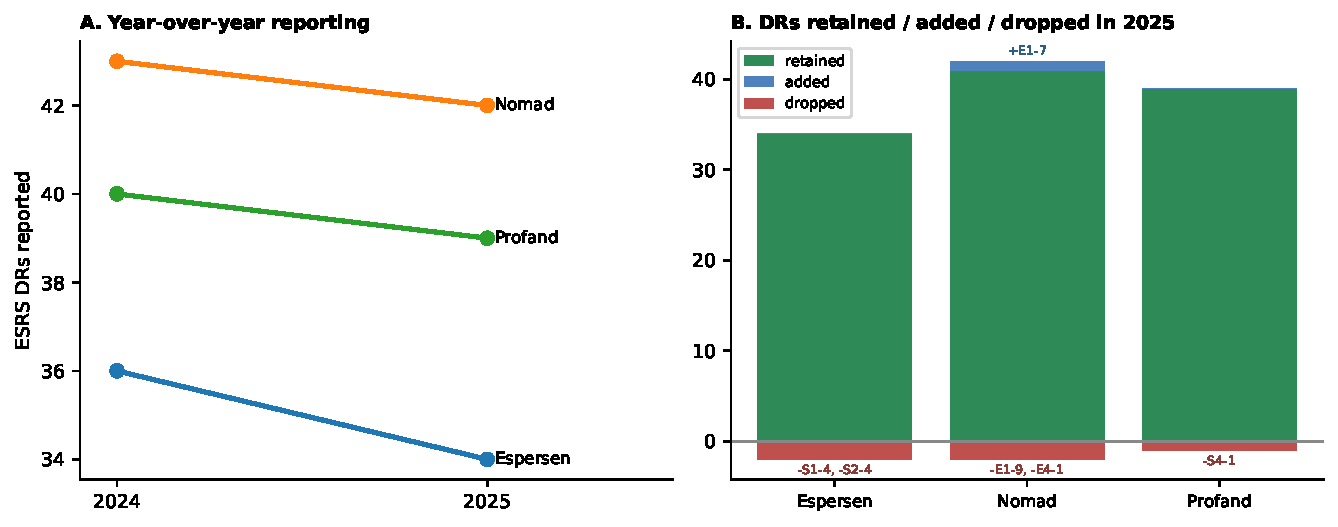
\includegraphics[width=\linewidth]{phase1/p1_year_evolution.pdf}
\caption{Year-over-year reporting for the three firms with both a 2024 and
a 2025 report. Panel~A: total requirements reported, on a zero-based axis, so
that the size of the change is not visually exaggerated. Panel~B: requirements
retained and dropped in 2025; no firm added a requirement. Change is dominated
by retention, with a small net reduction confined to three requirements across
the three firms.}
\label{fig:p1-year}
\end{figure}


\end{document}
